%!TEX program = xelatex
%!BIB program = biber
\documentclass[cn, 12pt, math=mtpro2, bibstyle=apa, blue]{elegantbook}
\title{高级微观经济学}
\subtitle{Advanced Microeconomics}
\version{0.2}
\prep{数学分析、高等代数、概率论、凸优化、微观经济学}

\setcounter{tocdepth}{3}
\cover{cover.png}

\date{\today}

\addbibresource[location=local]{reference.bib}

\usepackage{cprotect}
\usepackage{array}
\usepackage{bbm}
\usepackage{pgfplots}
\pgfplotsset{compat = newest}
\usetikzlibrary{positioning, arrows.meta}
\usepgfplotslibrary{fillbetween}
\newcommand{\ccr}[1]{\makecell{{\color{#1}\rule{1cm}{1cm}}}}

\definecolor{customcolor}{RGB}{233,233,233}
\colorlet{coverlinecolor}{customcolor}

\newcommand*{\rom}[1]{\expandafter\@slowromancap\romannumeral #1@}
\newcommand{\R}{\mathbb{R}}
\newcommand{\p}{\mathbf{p}}
\newcommand{\x}{\mathbf{x}}
\newcommand{\overbar}[1]{\mkern 1.5mu\overline{\mkern-1.5mu#1\mkern-1.5mu}\mkern 1.5mu}
\newcommand{\ubar}[1]{\mkern 1.5mu\underline{\mkern-1.5mu#1\mkern-1.5mu}\mkern 1.5mu}


\emergencystretch=4em
\begin{document}

\maketitle
\frontmatter

\tableofcontents

\mainmatter
\chapter{消费者理论\rom{1}}
\section{基本概念}
\textbf{消费集} (consumption set)消费者能想到的所有选择或者全部消费方案的集合, 不管其中的某些选择在现实中能否实现. 消费集也称选择集 (choice set), 用大写字母$X$表示.

假设每种商品是无限细分的, $x_i\in\R_+$表示商品$i$的数量, 这里假设每种商品数量非负且允许某些商品数量为0. 进一步, 假设有$n$种商品, 并用
$$\x=\begin{pmatrix}
      x_1 \\
      \vdots \\
      x_n
    \end{pmatrix}\in \R^n_+$$
表示含有$n$种商品的\textbf{消费束} (consumption bundle)或\textbf{消费计划} (consumption plan), $\R^n_+$称为商品空间 (commodity space). 因此, 消费束$\x\in X$可用$\R^n_+$中的点表示, 出于简单起见, 这里用整个$\R^n_+$表示消费集$X$.

\begin{postulate}\label{pos:pos1.1}
消费集的最低要求: 1. $X\subset \R_+^n$; 2. $X$是闭集和凸集; 3. $\mathbf{0}\in X$.
\end{postulate}

\textbf{可行集} (feasible set)是消费者脑海里能想到的, 并且在所处环境中所能得到的消费集, 用大写字母$B$表示, 它是$X$的真子集.

\textbf{偏好关系} (preference relation)为消费者的购买欲望, 反映消费者的主观愿望, 其为理想竞争市场的一个限制因素.
\section{偏好与效用}
\subsection{偏好关系}
消费者在$X$中的偏好关系$\succsim$可用来表示他对不同消费束的偏好, 如果$\x^1\succsim\x^2$, 那么对这个消费者来说, 称“$\x^1$至少和$\x^2$一样好”. 在消费者选择公理下, 消费者能够进行选择而且这些选择以某特定方式保持一致性.

进一步, 我们可以从偏好关系$\succsim$推导出$X$上的另外两种关系
\begin{itemize}
  \item 严格偏好关系 (strictly preference relation): $\x^1\succ \x^2 \Leftrightarrow \x^1\succsim \x^2$且$ \x^1\succsim \x^1$不成立, 称“$\x^1$严格好于$\x^2$”.
  \item 无差异关系 (indifference relation): $\x^1\sim \x^2 \Leftrightarrow \x^1\succsim \x^2$且$\x^2\succsim \x^1$, 称“$\x^1$和$\x^2$一样好”.
\end{itemize}
在大部分经济理论中, 经济学家都假设个人偏好是理性的 (rational), 这个假设体现在关于偏好关系$\succsim$的两个基本公理上, 即完备性公理和传递性公理.

\begin{axiom}[完备性]\label{axi:axi1.1}
对于任意$\x^1, \x^2\in X$, 要么$\x^1\succsim \x^2$, 要么$\x^2\succsim \x^1$.
\end{axiom}
完备性表明, 消费者具有分辨消费集内任意消费束的能力, 可以比较出是$\x^1$至少和$\x^2$一样好, 还是$\x^2$至少和$\x^1$一样好. 通常而言, 这条公理在现实中通常都是成立的.

\begin{axiom}[传递性]\label{axi:axi1.2}
对于$X$中的任意消费束$\x^1$, $\x^2$和$\x^3$, 如果$\x^1\succsim \x^2$且$\x^2\succsim\x^3$, 那么$\x^1\succsim\x^3$.
\end{axiom}
传递性要求消费者的选择必须一致. 然而, 这一公理是备受争议的, 人类的选择不总是传递的, 如果决策者评估的备选物不在他的常识范畴之内, 那么传递性这个公理很难得到满足, 但尽管如此还是认为传递性公理总是成立.

若把这两条公理结合起来, 这就意味着消费者能够将消费集$X$中的任何有限个元素全部排列起来, 排列顺序为从最好到最差, 当然可能会出现某些元素一样好的局面.
\begin{definition}[理性偏好关系]
如果消费集$X$上的偏好关系$\succsim$满足公理\ref{axi:axi1.1}和\ref{axi:axi1.2}, 则称$\succsim$为一个理性偏好关系.
\end{definition}
理性偏好关系$\succsim$是完备的和传递的, 蕴含着严格偏好$\succ$和无差异$\sim$的性质, 我们将这些性质总结在命题\ref{pro:pro1.1}中.
\begin{proposition}\label{pro:pro1.1}
  如果偏好关系$\succsim$是理性的, 那么下列结论成立
  \begin{enumerate}[\arabic*.]
    \item 如果$\x^1\succ\x^2\succsim\x^3$, 那么$\x^1\succ\x^3$;
    \item 如果$\x^1\succ\x^2$且$\x^2\succ\x^3$, 那么$\x^1\succ\x^3$;
    \item 如果$\x^1\sim\x^2$且$\x^2\sim\x^3$, 那么$\x^1\sim\x^3$并且$\x^2\sim \x^1$.
  \end{enumerate}
\end{proposition}
\begin{proof}
  1. 由于$\x^1\succ\x^2$意味着$\x^1\succsim \x^2$, 传递性表明$\x^1\succsim \x^3$. 假设$\x^3\succsim\x^1$, 由于$\x^2\succsim \x^3$, 因此传递性意味着$\x^2\succsim \x^1$, 但这与$\x^1\succ \x^2$矛盾, 故而只有$\x^1\succ\x^3$.

  2. 原理同上.

  3. 假设$\x^1\sim\x^2$且$\x^2\sim\x^3$, 那么$\x^1\succsim\x^2$, $\x^2\succsim\x^3$, $\x^2\succsim\x^1$, $\x^3\succsim\x^2$, 传递性意味着$\x^1\succsim\x^3$且$\x^3\succsim\x^1$, 也即$\x^1\sim\x^3$. 另一方面, $\x^1\sim \x^2$意味着$\x^2\succsim\x^1$且$\x^1\succsim\x^2$, 也即$\x^2\sim\x^1$.
\end{proof}
\begin{definition}
设$\x^0$是消费集$X$内的任意一点, 与$\x^0$相联系, 可以定义$X$的子集
\begin{enumerate}[label=\arabic*.]
  \item $\succsim(\x^0)\equiv \{\x: \x\in X, \x\succsim\x^0\}$, 称为“至少和$\x^0$一样好”的集合;
  \item $\precsim(\x^0)\equiv \{\x: \x\in X, \x^0\succsim\x\}$, 称为“不比$\x^0$好”的集合;
  \item $\succ(\x^0)\equiv \{\x: \x\in X, \x\succ\x^0\}$, 称为“比$\x^0$好”的集合;
  \item $\prec(\x^0)\equiv \{\x: \x\in X, \x^0\succ \x\}$, 称为“比$\x^0$差”的集合;
  \item $\sim(\x^0)\equiv\{\x: \x\in X, \x\sim \x^0\}$, 称为“与$\x^0$无差异”的集合.
\end{enumerate}
\end{definition}

对于消费集$X=\R_+^2$, 图\ref{fig1.1}表示了一个理性的虚拟偏好集, $X$中的任意一点$\x^0=(x_1^0,x_2^0)'$表示该消费束中商品1和2的数量分别为$x_1^0$和$x_2^0$, 并且集合$\succ(\x^0)$, $\prec(\x^0)$和$\sim(\x^0)$将整个$X$划分为了三个互不相交的子集.
\begin{figure}
  \centering
  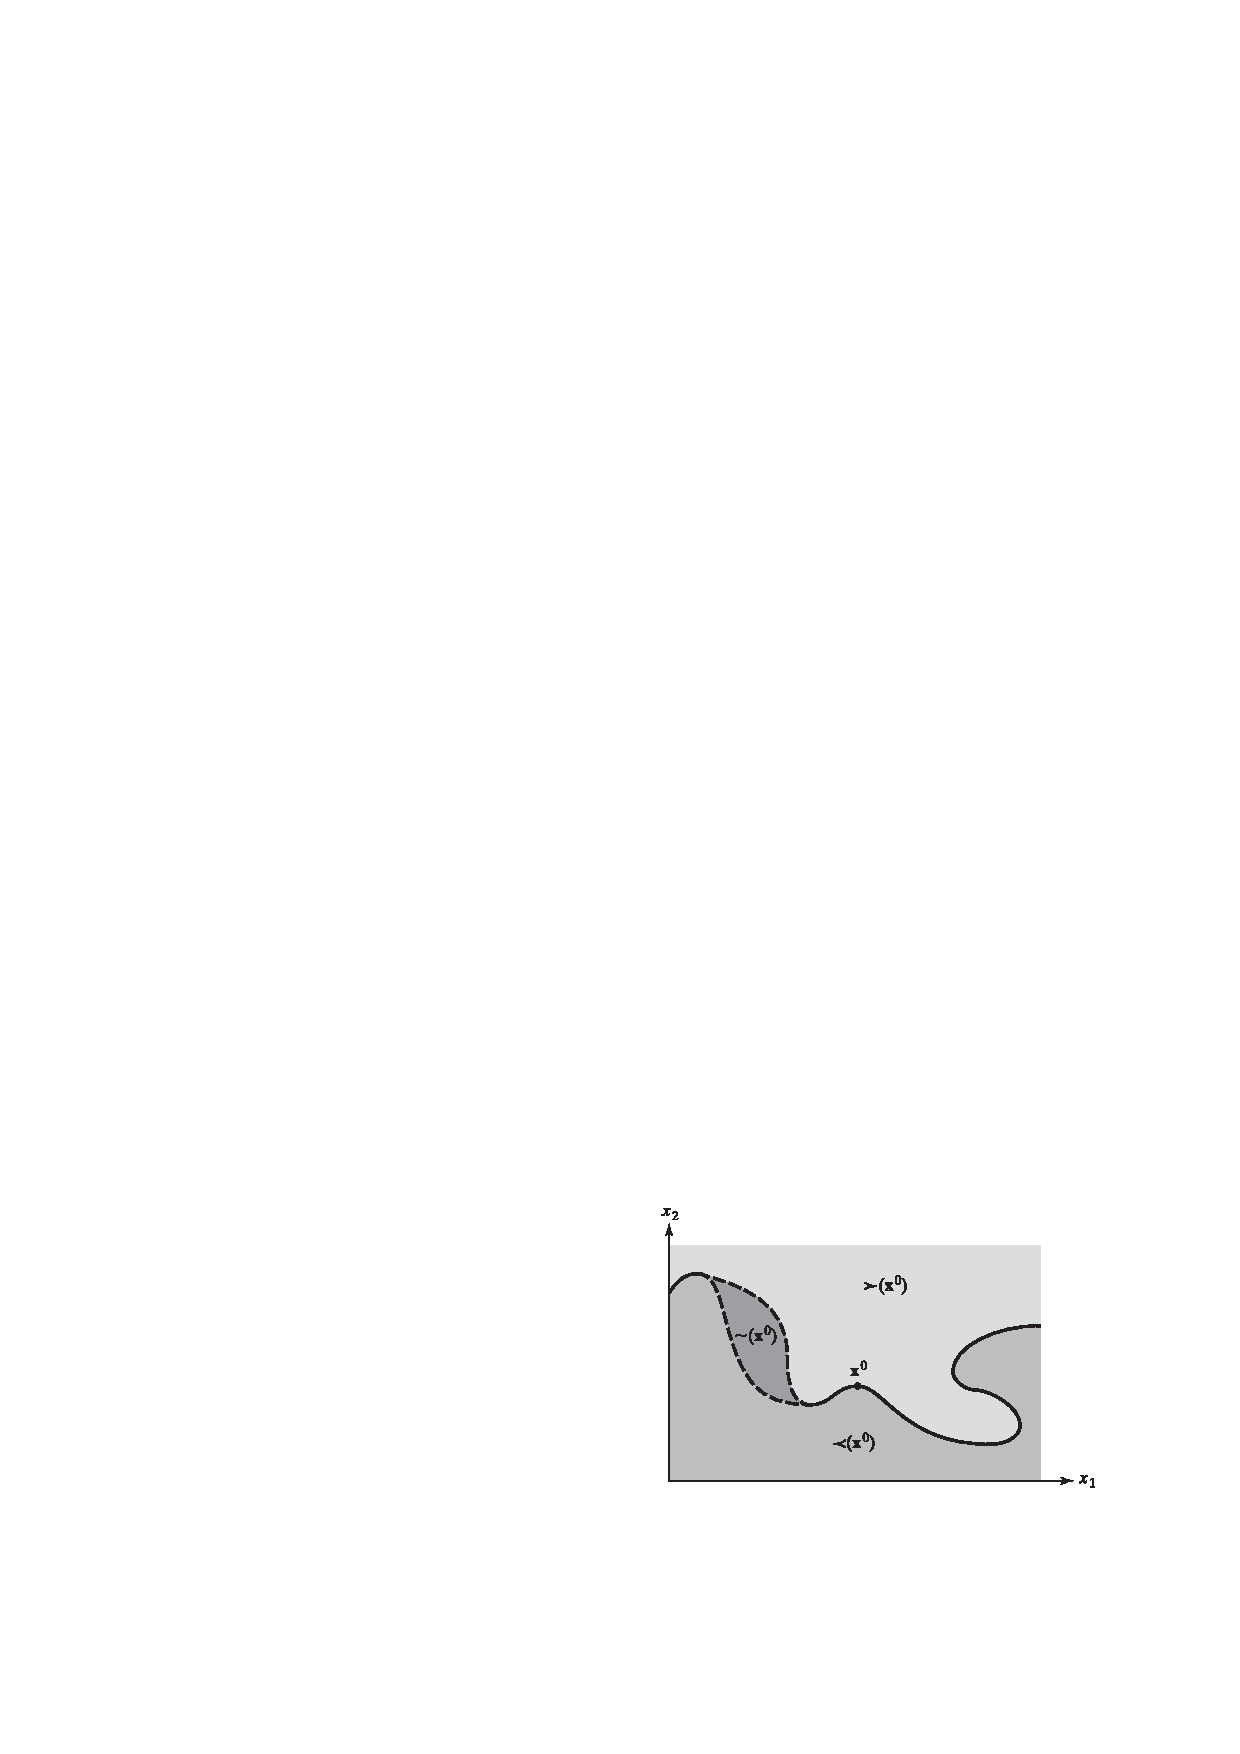
\includegraphics[width=10cm]{fig1-1.pdf}
  \caption{理性虚拟偏好.}\label{fig1.1}
\end{figure}

由于还未给出其它公理, 理性偏好允许了图\ref{fig1.1}中不规则区域的存在, 例如无差异区域内部的空隙. 以下明确地将消费集设置为$X=\R^n_+$.

\begin{axiom}[连续性]\label{axi:axi1.3}
对于任意$\x\in\R^n_+$, 集合$\succsim(\x)$和$\precsim(\x)$在$\R_+^n$中是闭的.
\end{axiom}
连续性公理保证了偏好不会发生突然逆转. 如果消费束序列中的每个元素$\mathbf{y}^n$至少与$\x$一样好, 并且$\mathbf{y}^n$收敛于$\mathbf{y}$, 则$\mathbf{y}$至少与$\x$一样好. 由于$\succsim(\x)$和$\precsim(\x)$是闭的, 因此它们的交集$\sim(\x)$也是闭的, 这就排除了图\ref{fig1.1}中虚线的存在, 图\ref{fig1.2}画出了满足连续性的理性虚拟偏好.

\begin{figure}[htbp!]
  \centering
  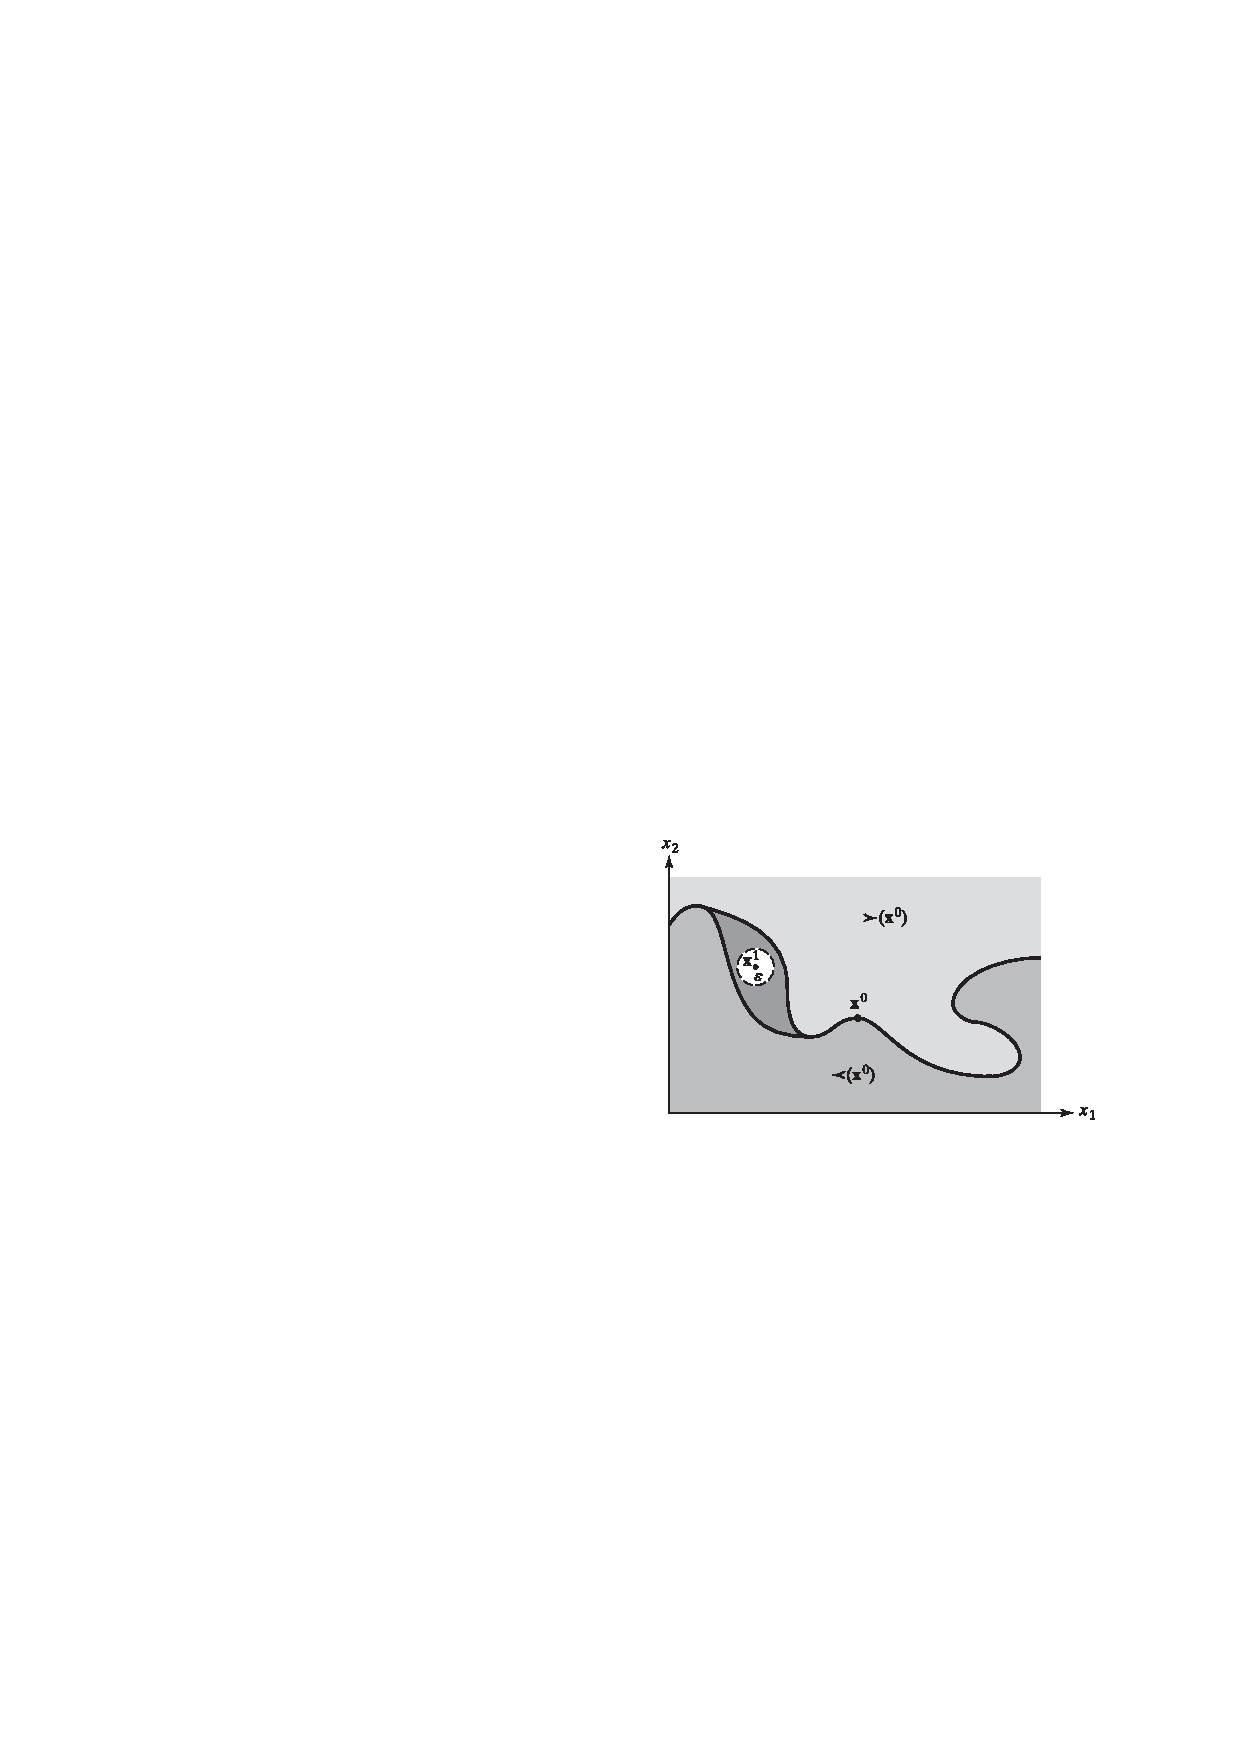
\includegraphics[width=10cm]{fig1-2.pdf}
  \caption{满足公理\ref{axi:axi1.3}的理性虚拟偏好.}\label{fig1.2}
\end{figure}

\begin{example}[字典偏好关系]
假设$X=\R_+^2$, 将偏好关系$\succsim$定义为要么$x_1>y_1$, 要么$x_1=y_1$且$x_2\ge y_2$, 则称$\succsim$是字典偏好关系. 可以证明, 字典偏好关系不是连续的.
\end{example}

接下来的几条假设将使的偏好的结构更复杂但更规则, 如果说前面的三条公理是必须的, 那么下面的这类假设则要根据具 体研究的选择决策问题来决定是否使用. 在下面每类假设中, 先介绍较弱的公理, 然后再介绍较强的公理.

\begin{axiom}[局部非饱和性]\label{axi:axi1.4}
对于任意$\x^0\in\R^n_+$以及$\epsilon>0$, 总存在$\x\in B_\varepsilon(\x^0)\cap \R_+^n$, 使得$\x\succ\x^0$.
\end{axiom}
局部非饱和性排除了无差异区域的存在, 因为在无差异区域中, 总能找到某个$\epsilon>0$和$B_\epsilon(\x^1)$, 使得$B_\epsilon(\x^1)$中的点和$\x^1$无差异, 如图\ref{fig1.3}所示.
\begin{figure}
  \centering
  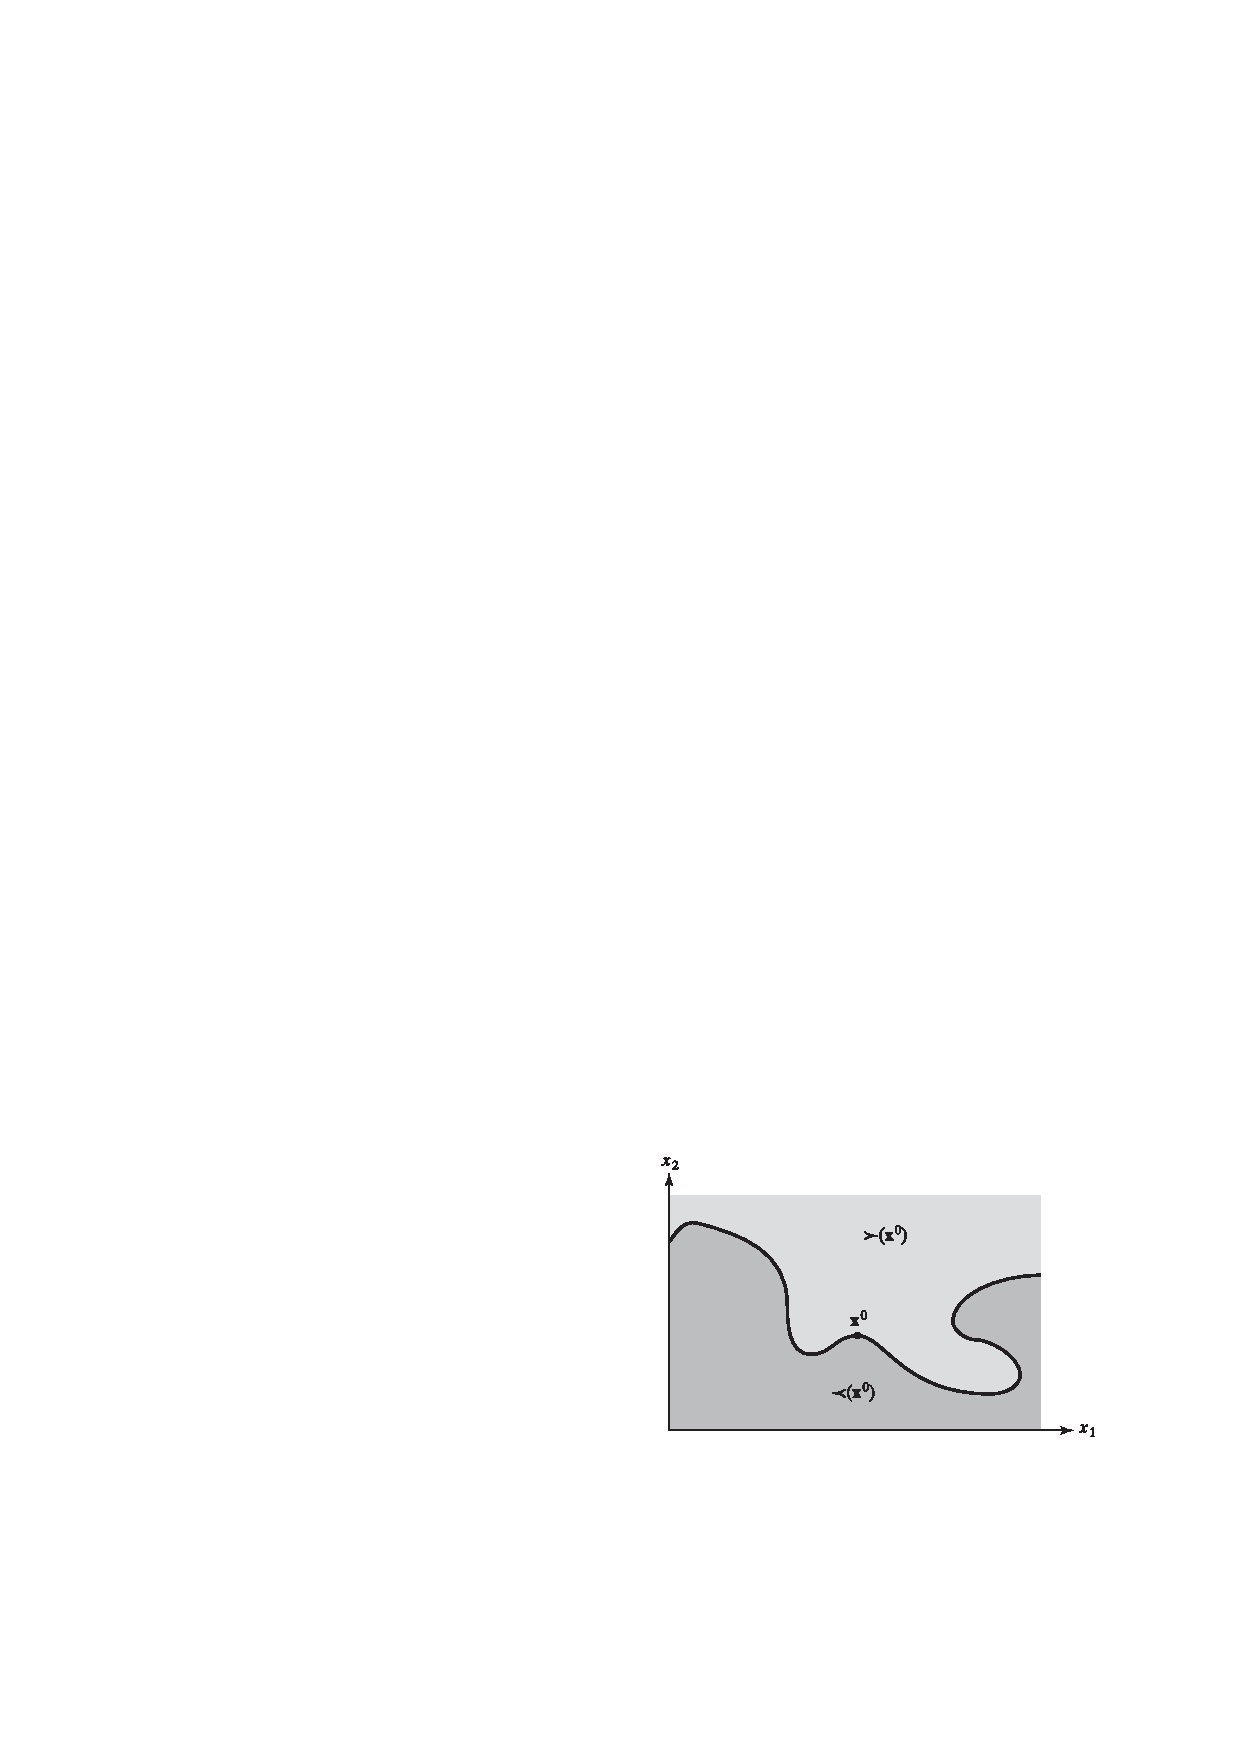
\includegraphics[width=10cm]{fig1-3.pdf}
  \caption{满足公理\ref{axi:axi1.3}和\ref{axi:axi1.4}的理性虚拟偏好.}\label{fig1.3}
\end{figure}

然而, 这并不意味着增加所有商品的数量必然能使消费者的状况更好, 以下更强的严格单调性公理则表明了这一点.

\begin{axiom}[严格单调性]\label{axi:axi1.5}
对于任意$\x^0,\x^1\in\R^n_+$, 如果$\x^0\ge\x^1$, 那么$\x^0\succsim \x^1$; 如果$\x^0\gg\x^1$, 那么$\x^0\succ\x^1$.
\end{axiom}
严格单调性表明如果某消费束的每种商品数量至少和另一个消费束的一样多, 则该消费束至少和它一样好; 如果某消费束的每种商品严格多于另一个消费束, 则该消费束比后者好. 此外, 这一公理排除了$\R^2_+$中无差异集中的向上弯曲部分和斜率为正的部分, 如图\ref{fig1.4}所示.

\begin{figure}
  \centering
  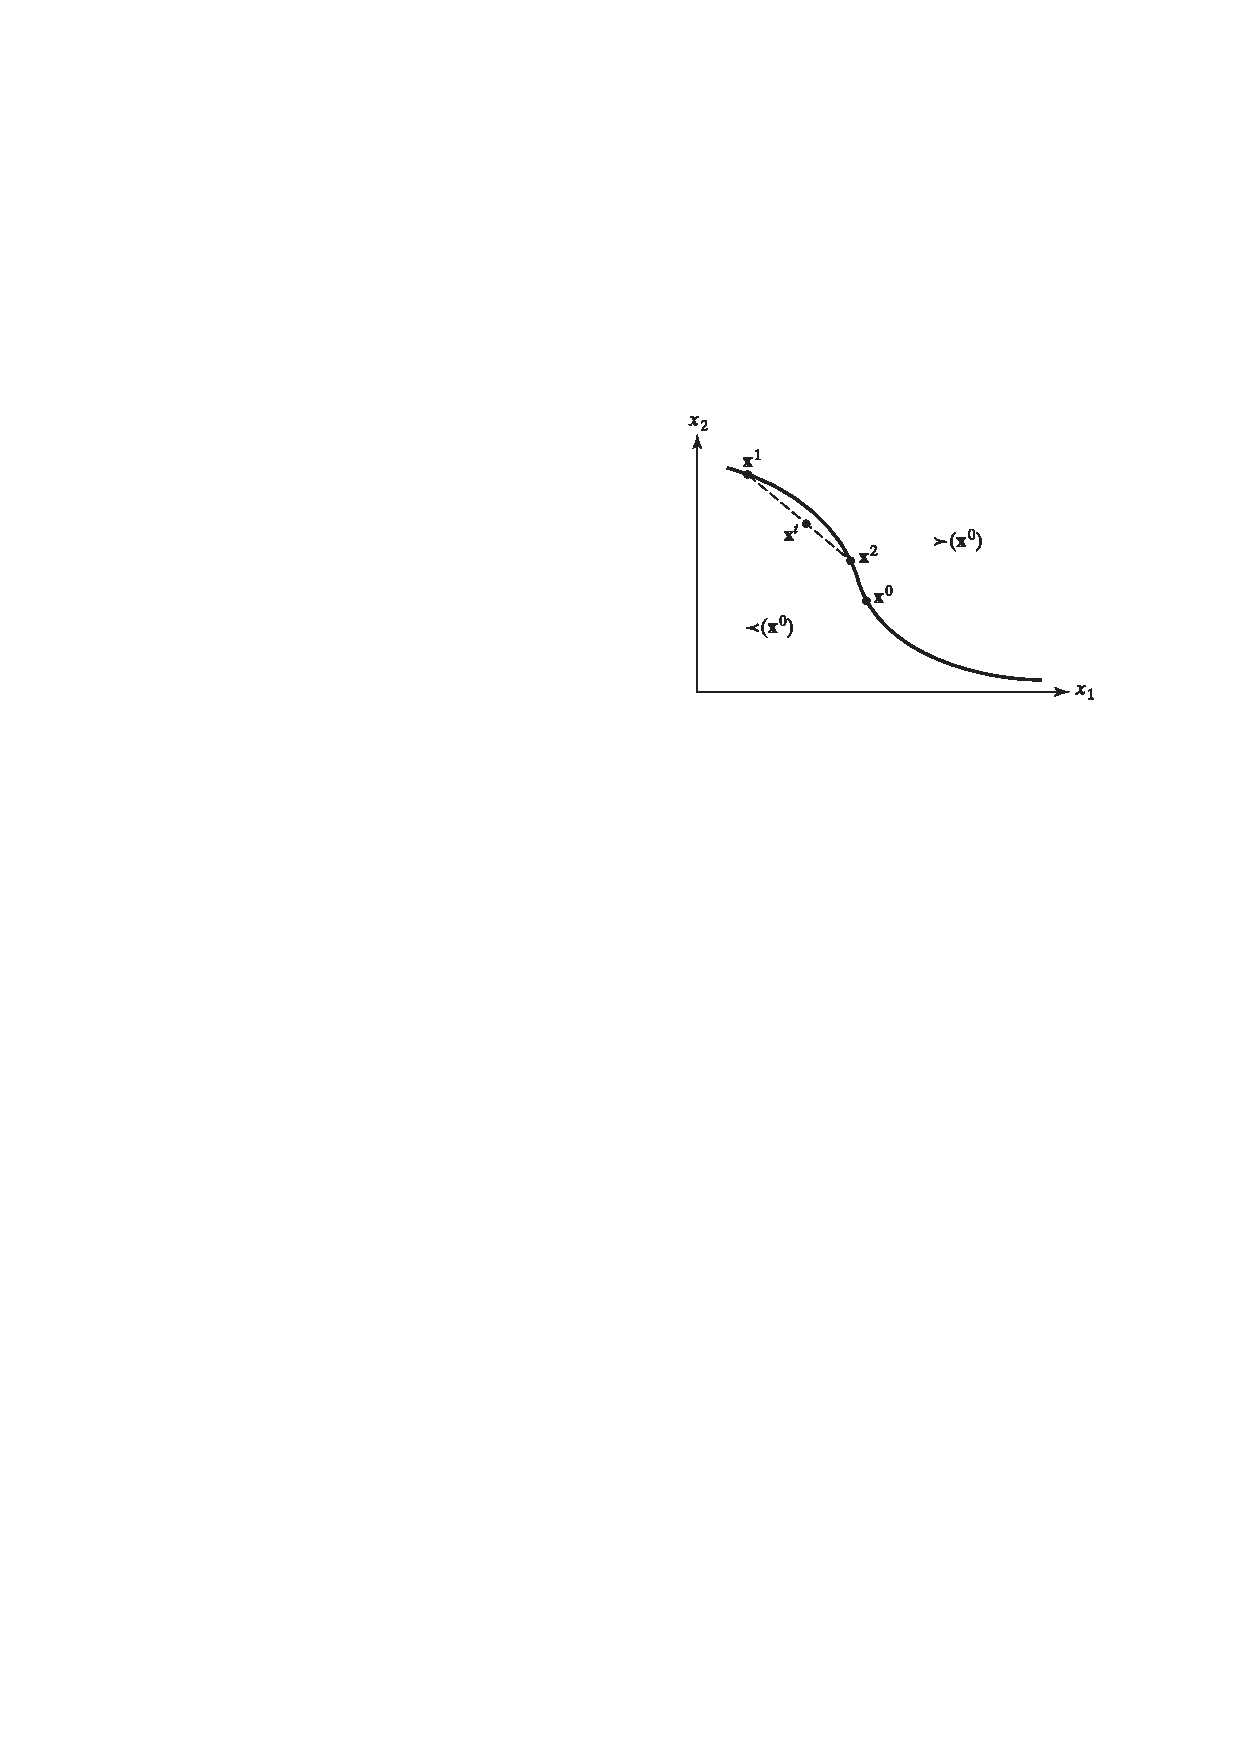
\includegraphics[width=10cm]{fig1-4.pdf}
  \caption{满足公理\ref{axi:axi1.3}和\ref{axi:axi1.5}的理性虚拟偏好.}\label{fig1.4}
\end{figure}

\begin{axiom}[凸性]\label{axi:axi1.6}
如果$\x^1\succsim\x^0$, 则对于一切$t\in[0,1]$都有$t\x^1+(1-t)\x^0\succsim\x^0$.
\end{axiom}
\begin{axiom}[严格凸性]\label{axi:axi1.7}
如果$\x^1\ne\x^0$且$\x^1\succsim\x^0$, 则对于一切$t\in(0,1)$都有$t\x^1+(1-t)\x^0\succ\x^0$.
\end{axiom}

如果凸性或严格凸性与公理\ref{axi:axi1.1}、\ref{axi:axi1.2}、\ref{axi:axi1.3}和\ref{axi:axi1.5}联合起来, 那么可以排除图\ref{fig1.4}中西北方向凹向原点的部分, 如图\ref{fig1.5}所示.

对于我们将要构造的消费者理论来说, 引入公理\ref{axi:axi1.6}不会造成理论一般性的任何损失. 引入或不引入这个公理, 消费者理论的内容是相同的. 若引入公理\ref{axi:axi1.7}, 则多少会造成一般性的损失, 但是它可以大幅简化我们的分析.

描述凸偏好的另一种方式是\textbf{曲率} (curvature), 当消费集为$X=\R^2_+$, 无差异曲线的斜率称为商品1对商品2的\textbf{边际替代率} (Marginal Rate of Substitution, MRS), 它衡量为了维持相同的效用水平, 消费者减少1单位商品1的消费, 应该补偿给她多少商品2.

当公理\ref{axi:axi1.6}成立时, 如果沿着无差异曲线从西北到东南移动, 那么MRS不变或递减, 而如果公理\ref{axi:axi1.7}成立, 则要求MRS严格递减. 凸偏好的这种性质称为边际替代率递减规律.
\begin{figure}
  \centering
  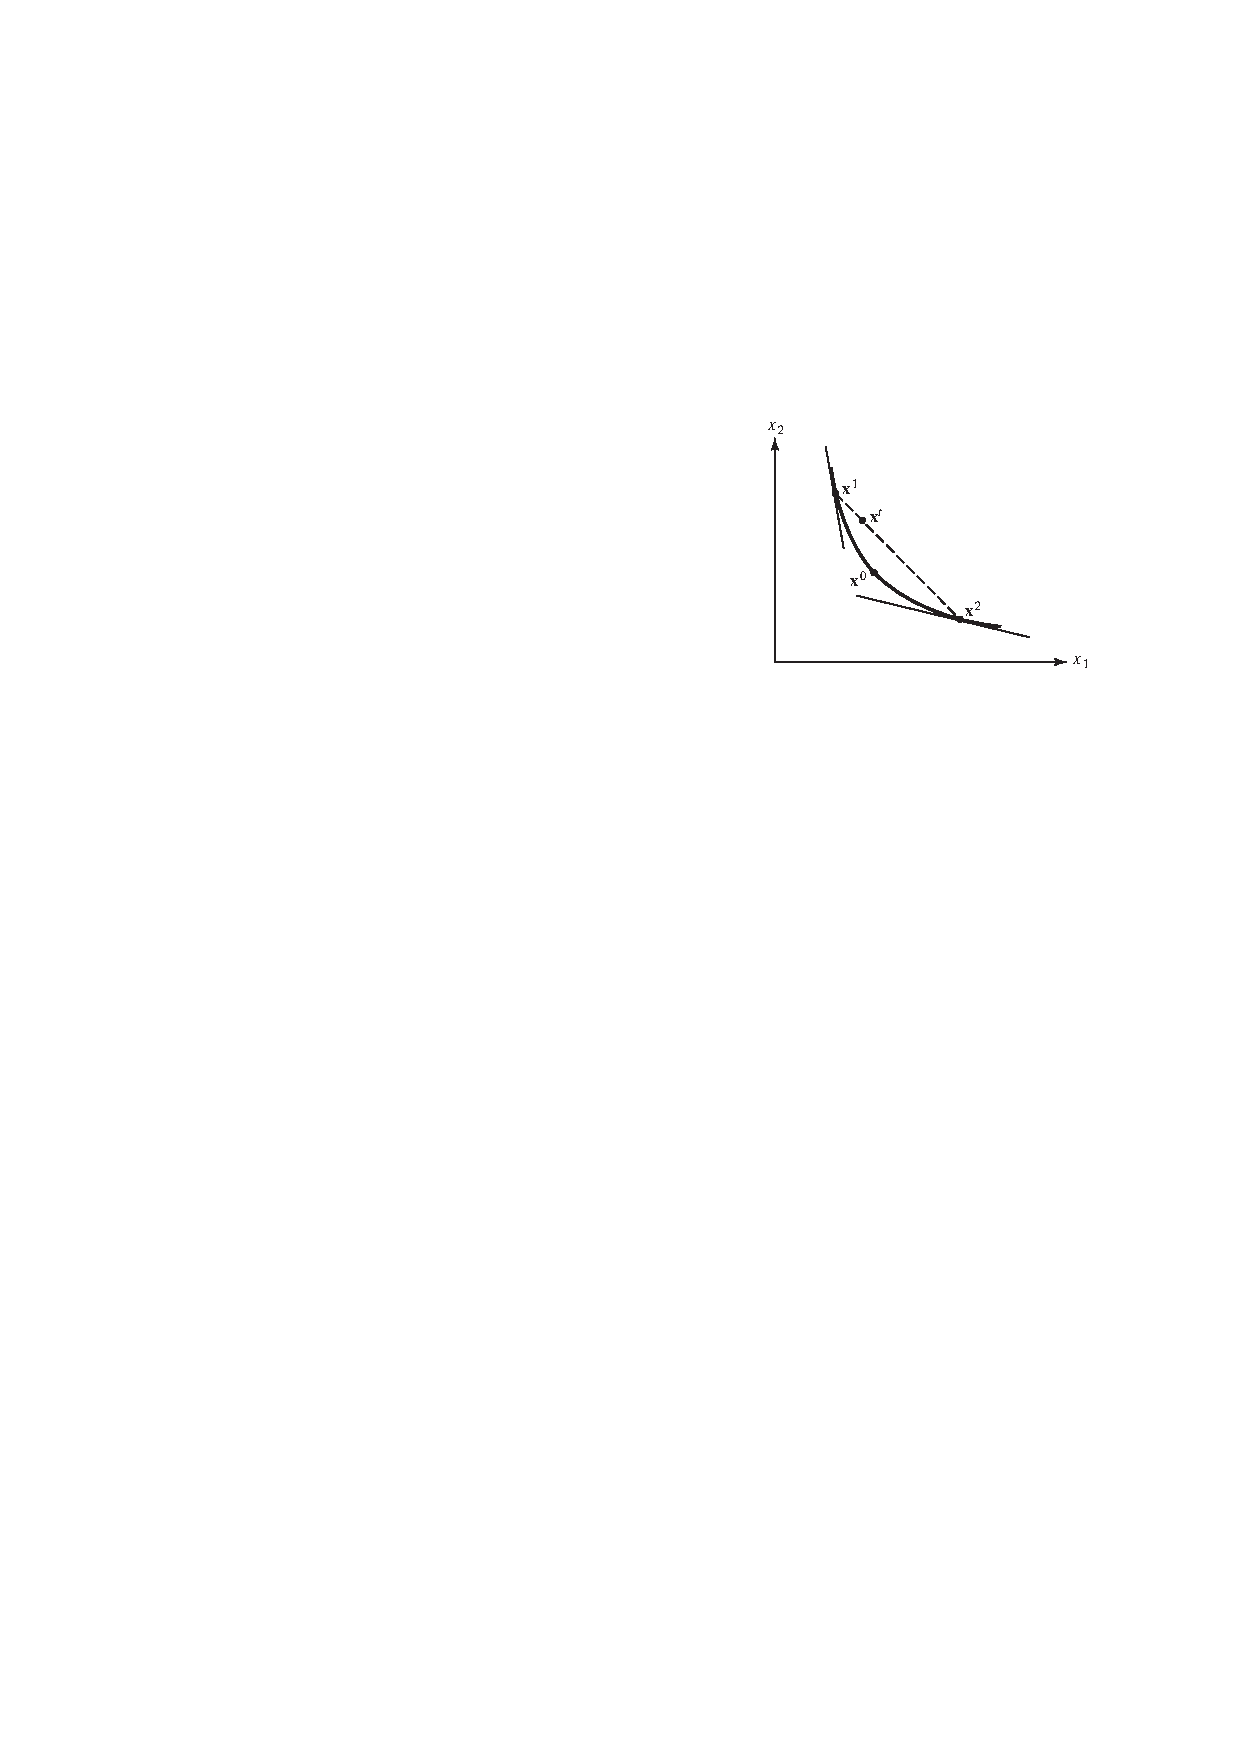
\includegraphics[width=10cm]{fig1-5.pdf}
  \caption{满足公理\ref{axi:axi1.3}、\ref{axi:axi1.5}、\ref{axi:axi1.6}或\ref{axi:axi1.7}的理性虚拟偏好.}\label{fig1.5}
\end{figure}
\subsection{效用函数}
\begin{definition}
实值函数$u:\R_+^n\to\R$称为表示偏好关系$\succsim$的效用函数 (utility function), 如果对于一切$\x^0, \x^1\in\R^n_+$, 都有$u(\x^0)\ge u(\x^1)\Leftrightarrow \x^0\succsim\x^1$.
\end{definition}
表示偏好关系$\succsim$的效用函数不是唯一的, 对于任意严格递增的单调函数$f:\R\to\R$来说, $v(\x)=f(u(\x))$都是一个新的效用函数, 它与$u(\x)$表示的偏好相同. 效用函数这种不随任何严格递增变换而改变的性质称为\textbf{序数} (ordinal)性质, 而\textbf{基数} (cardinal)性质则是指在这样的变换下不能保留的性质.

\begin{proposition}
只有理性偏好才能用效用函数表示.
\end{proposition}
\begin{proof}
 只需证明若存在能表示偏好关系$\succsim$的效用函数, 则$\succsim$必然满足公理\ref{axi:axi1.1}和\ref{axi:axi1.2}.

 因为$u$是定义在$\R_+^n$上的实值函数, 那么对于任意$\x,\mathbf{y}\in\R_+^n$, 必有$u(\x)\ge u(\mathbf{y})$或$u(\x)\le u(\mathbf{y})$, 由于$u$是表示偏好关系$\succsim$的效用函数, 因此$\x\succsim \mathbf{y}$和$\mathbf{y}\succsim\x$总有一个成立, 也即偏好关系$\succsim$满足公理\ref{axi:axi1.1}.

 假设对于任意$\x, \mathbf{y}, \mathbf{z}\in\R_+^n$都有$\x\succsim\mathbf{y}$且$\mathbf{y}\succsim\mathbf{z}$, 那么$u(\x)\ge u(\mathbf{y})$且$u(\mathbf{y})\ge u(\mathbf{z})$, 也即$u(\x)\ge u(\mathbf{z})$, 因为$u$表示了偏好关系$\succsim$, 故而$\x\succsim\mathbf{z}$, 也即公理\ref{axi:axi1.2}成立.
\end{proof}

\begin{theorem}\label{thm:thm1.1}
  如果理性偏好$\succsim$是连续和严格单调的, 那么存在可以代表$\succsim$的连续效用函数$u:\R^n_+\to\R$.
\end{theorem}
\begin{proof}
  令$\mathbf{e}=(1,\cdots,1)'\in\R^n_+$为单位向量, 首先证明存在映射$u:\R^n_+\to\R$, 使得$u(\x)\mathbf{e}\sim \x$.

  固定消费束$\x\in\R^n_+$, 根据连续性公理可知集合
  \begin{align*}
  A^+&=\{t\ge0: t\mathbf{e}\succsim \x\} \\
  A^-&=\{t\ge0: t\mathbf{e}\precsim \x\}
  \end{align*}
  都是非空闭集. 由于偏好关系$\succsim$是完备的, 故而$\R_+\subset A^+\cup A^-$, 又因为$A^+$和$A^-$是闭的, 并且$\R_+$是连通的, 所以$A^+\cap A^-\neq\emptyset$, 于是存在$t\ge0$使得$t\mathbf{e}\sim \x$. 假设还存在另一个$t'\ge0$使得$t'\mathbf{e}\sim \x$, 根据命题\ref{pro:pro1.1}可知$t\mathbf{e}\sim t'\mathbf{e}$, 于是由严格单调性知$t=t'$, 也即这样的$t$是唯一的.

  由上面的论证可知, 对于任意$\x\in\mathbb{R}_+^n$, 总存在唯一的实数$u(\x)$使得$u(\x)\mathbf{e}\sim\x$, 下面证明$u$代表了偏好关系$\succsim$. 给定消费束$\x^1, \x^2\in\R_+^n$, 于是
  \begin{align*}
  \x^1\succsim\x^2&\Leftrightarrow u(\x^1)\mathbf{e}\sim \x^1\succsim u(\x^2)\mathbf{e}\sim \x^2 \\
  &\Leftrightarrow u(\x^1)\mathbf{e}\succsim u(\x^2)\mathbf{e} \\
  &\Leftrightarrow u(\x^1)\ge u(\x^2)
  \end{align*}
  这就得到了可以表示偏好关系$\succsim$的效用函数的存在性.

  最后需要证明效用函数$u:\R^n_+\to \R$是连续的, 注意到对于每个$a<b$都有
  \begin{align*}
  u^{-1}((a,b))&=\{\x: a<u(\x)<b\} \\
  &=\{\x: a\mathbf{e}\prec u(\x)\mathbf{e}\prec b\mathbf{e}\} \\
  &=\{\x: a\mathbf{e}\prec \x\mathbf{e}\prec b\mathbf{e}\} \\
  &=\succ (a\mathbf{e})\,\,\cap \prec(b\mathbf{e})
  \end{align*}
  根据连续性可知$\succ(a\mathbf{e})$和$\prec(b\mathbf{e})$是开的, 由于开集的交也是开的, 因此$u^{-1}((a,b))$是开的, 故而由连续函数的定义可知$u$是连续的.
\end{proof}

连续的理性偏好排除了病态的效用函数, 但是它没有排除出现拐折 (kink)函数情形, 例如Leontief偏好, 而如果效用函数是可微的, 那么无差异曲线不仅是连续曲线, 并且还是光滑的. 因此, 效用函数的可微性比连续性要求更高, 可微效用函数也不一定能表示某些连续偏好, 但通常在需要的时候就假设$u$是可微的.


当效用函数可微时, $u(\x)$对$x_i$的一阶偏导为商品$i$的\textbf{边际效用} (marginal utility), 考虑任意消费束$\x^1=(x^1_1,x^2_2)$, 因为经过点$\x^1$的无差异曲线是平面$(x_1,x_2)$的函数, 令$x_2=f(x_1)$为这一函数, 因此当效用水平维持在常数时, 对于一切$\x\in\R_+$都有
\begin{equation}\label{eq1.1}
  u(x_1,f(x_1))=\text{常数}
\end{equation}
对于消费束$\x^1=(x^1_1,x^1_2)$, 商品1替代商品2的边际替代率$\text{MRS}_{12}$为经过点$(x_1^1,x_2^1)$的无差异曲线在该点的斜率的绝对值, 也即
$$\text{MRS}_{12}(x_1^1,x_2^1)=|f'(x_1^1)|=-f'(x_1^1)$$
在式(\ref{eq1.1})中对$x_1$求微分
\begin{equation}\label{eq1.2}
  \frac{\partial u}{\partial x_1}+\frac{\partial u}{\partial x_2}f'(x_1)=0
\end{equation}
根据式(\ref{eq1.1})和(\ref{eq1.2})可得
$$\text{MRS}_{12}(\x^1)=\frac{\partial u(\x^1)/\partial x_1}{\partial u(\x^1)/\partial x_2}$$
一般地, 对于某个消费者来说, 商品$i$对商品$j$的边际替代率为
$$\text{MRS}_{ij}(\x)=\frac{\partial u(\x)/\partial x_i}{\partial u(\x)/\partial x_j}=\left|\frac{\text{d}x_j}{\text{d}x_i}\right|$$
其中$i,j=1,\cdots,n$. 上式表明如果想让消费者在边际上减少一单位商品$i$的消费, 我们应该补偿给他多少单位商品$j$.

当$u(\x)$在$\R^n_{++}$上可微并且它表示的偏好关系$\succsim$严格单调时, 每种商品的边际效用“几乎”严格为正,\footnote{“几乎”表示除开Lebesgue测度为0的消费束$\x$.} 也即几乎对于一切消费束$\x$都有$\partial u(\x)/\partial x_j>0$. 更一般地, 对于任何拟凹效用函数, 由它的二阶偏导构成的Hessian矩阵$\mathbf{H}(\x)$满足
$$\mathbf{y}'\mathbf{H}(\x)\mathbf{y}\le0,\quad \nabla u(\x)\cdot\mathbf{y}=0$$

  \begin{theorem}\label{thm:thm1.2}
    设偏好关系$\succsim$可由效用函数$u:\R_+^n\to\R$表示, 则以下结论成立:
    \begin{enumerate}[label=\arabic*.]
      \item $u$是严格递增函数当且仅当$\succsim$是严格单调的;
      \item $u$是拟凹函数当且仅当$\succsim$是凸的;
      \item $u$是严格拟凹函数当且仅当$\succsim$是严格凸的.
    \end{enumerate}
  \end{theorem}
  \begin{proof}
    1. 设$\x\ge \mathbf{y}$且$u$是严格递增的, 于是$u(\x)\geq (\mathbf{y})\Leftrightarrow \x\succsim \mathbf{y}$; 反之, 如果$\succsim$是严格单调的, 那么当$\x\ge\mathbf{y}$是有$\x\succsim\mathbf{y}$, 从而$u(\x)\ge u(\mathbf{y})$, 也即$u$是严格递增的.

    2. 设$u$是拟凹函数, 也即对于任意$t\in [0,1]$都有$u(t\x+(1-t)\mathbf{y})\geq \min\{u(\x), u(\mathbf{y})\}$. 不妨设$\x\succsim \mathbf{y}$, 从而$t\x+(1-t)\mathbf{y}\succsim \mathbf{y}$, 也即$\succsim$是凸的; 反之, 假设$\succsim$是凸的并且$\x\succsim\mathbf{y}$, 于是由1.可知$u(\x)\ge u(\mathbf{y})$, 并且对于一切$t\in[0,1]$都有$t\x+(1-t)\mathbf{y}\succsim \mathbf{y}$, 从而$u(t\x+(1-t)\mathbf{y})\geq \min\{u(\x), u(\mathbf{y})\}$, 也即$u$是拟凹的.

    3. 证明同上.
  \end{proof}
  值得注意的是, 偏好关系$\succsim$的凸性并不意味着$u$是凹的, 凹性是比拟凹更强的性质. 事实上, 对于某个特定的凸偏好关系$\succsim$, 可能不存在任何能代表这个偏好关系的凹效用函数.
\section{消费者问题}
\begin{postulate}\label{pos:pos1.2}
理性偏好关系$\succsim$在$\R_+^n$是连续的, 严格单调和严格凸的.
\end{postulate}
在以上假设成立的条件下, 由定理\ref{thm:thm1.1}和\ref{thm:thm1.2}可知这个偏好关系可用连续实值函数$u:\R^n_+\to\R$表示, 并且$u$在$\R^n_+$是连续、严格递增和严格拟凹的, 此时的无差异曲线如图\ref{fig1.6}所示. 无差异曲线满足: (1)离原点越远的效用水平越高; (2)凸向原点; (3)不同的无差异曲线不相交.
\begin{figure}[htbp!]
  \centering
  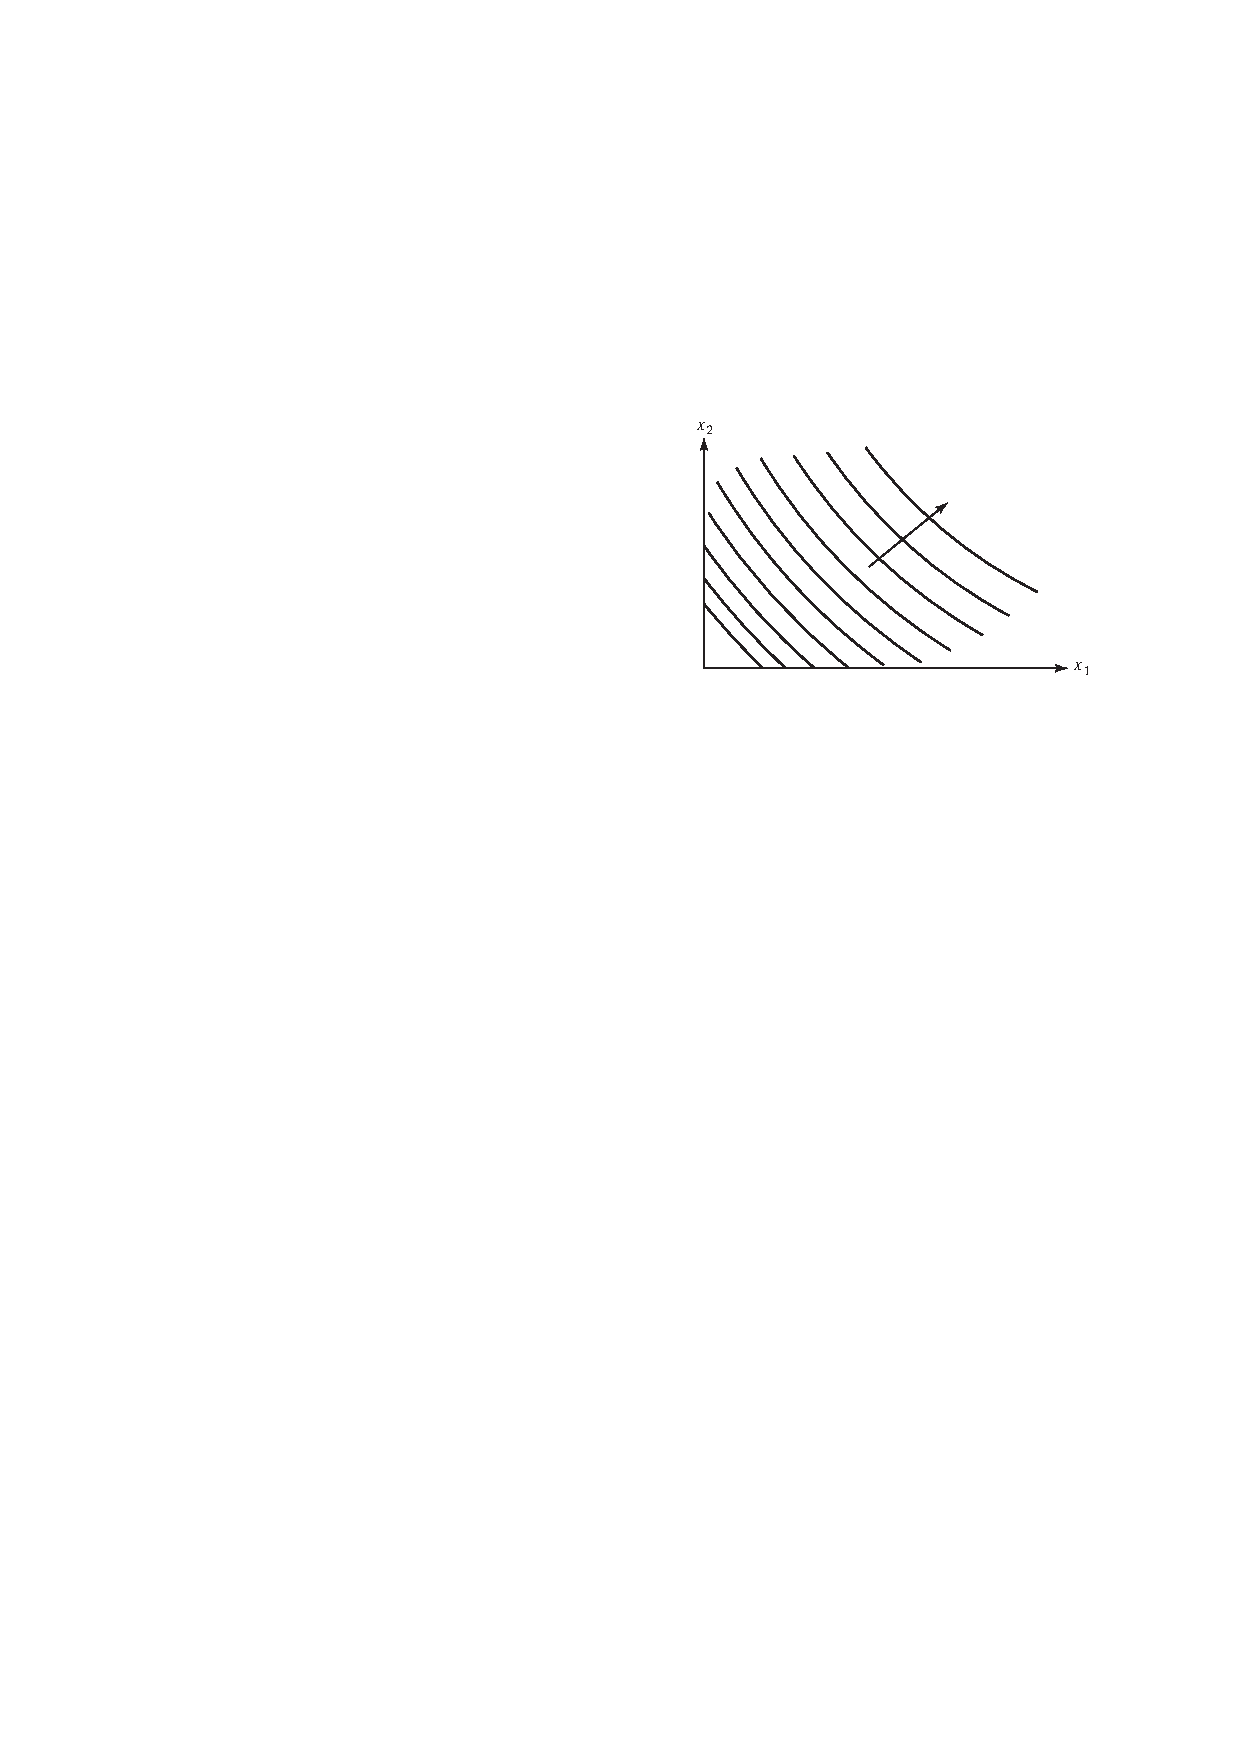
\includegraphics[width=10cm]{fig1-6.pdf}
  \caption{满足假设\ref{pos:pos1.2}的无差异曲线}\label{fig1.6}
\end{figure}

接下来假设消费者所处的环境是市场经济, 它是一个经济系统, 人与人之间的交易是在这一市场中进行的, 每种商品$i$都有自己的市场且价格$p_i>0$, 而且消费者在每个市场的影响力很小, 市场价格$\p\gg\mathbf{0}$是固定不变的. 消费者所处经济环境的假设可由\textbf{预算集} (budget set)表示.
\begin{definition}\label{def:def1.3}
消费者的预算集是$B=\{\x\in\R_+^n: \mathbf{p}\cdot\x\leq y\}$.
\end{definition}
在定义\ref{def:def1.3}中
$$\p\cdot\x=\sum_{i=1}^{n}p_ix_i$$
表明消费者的预算不能超过它所拥有的全部财富$y\in \R_+$. 在只有两种商品的情况下, 预算集$B$由图\ref{fig1.7}的阴影部分和边界上的消费束构成.
\begin{figure}[htbp!]
  \centering
  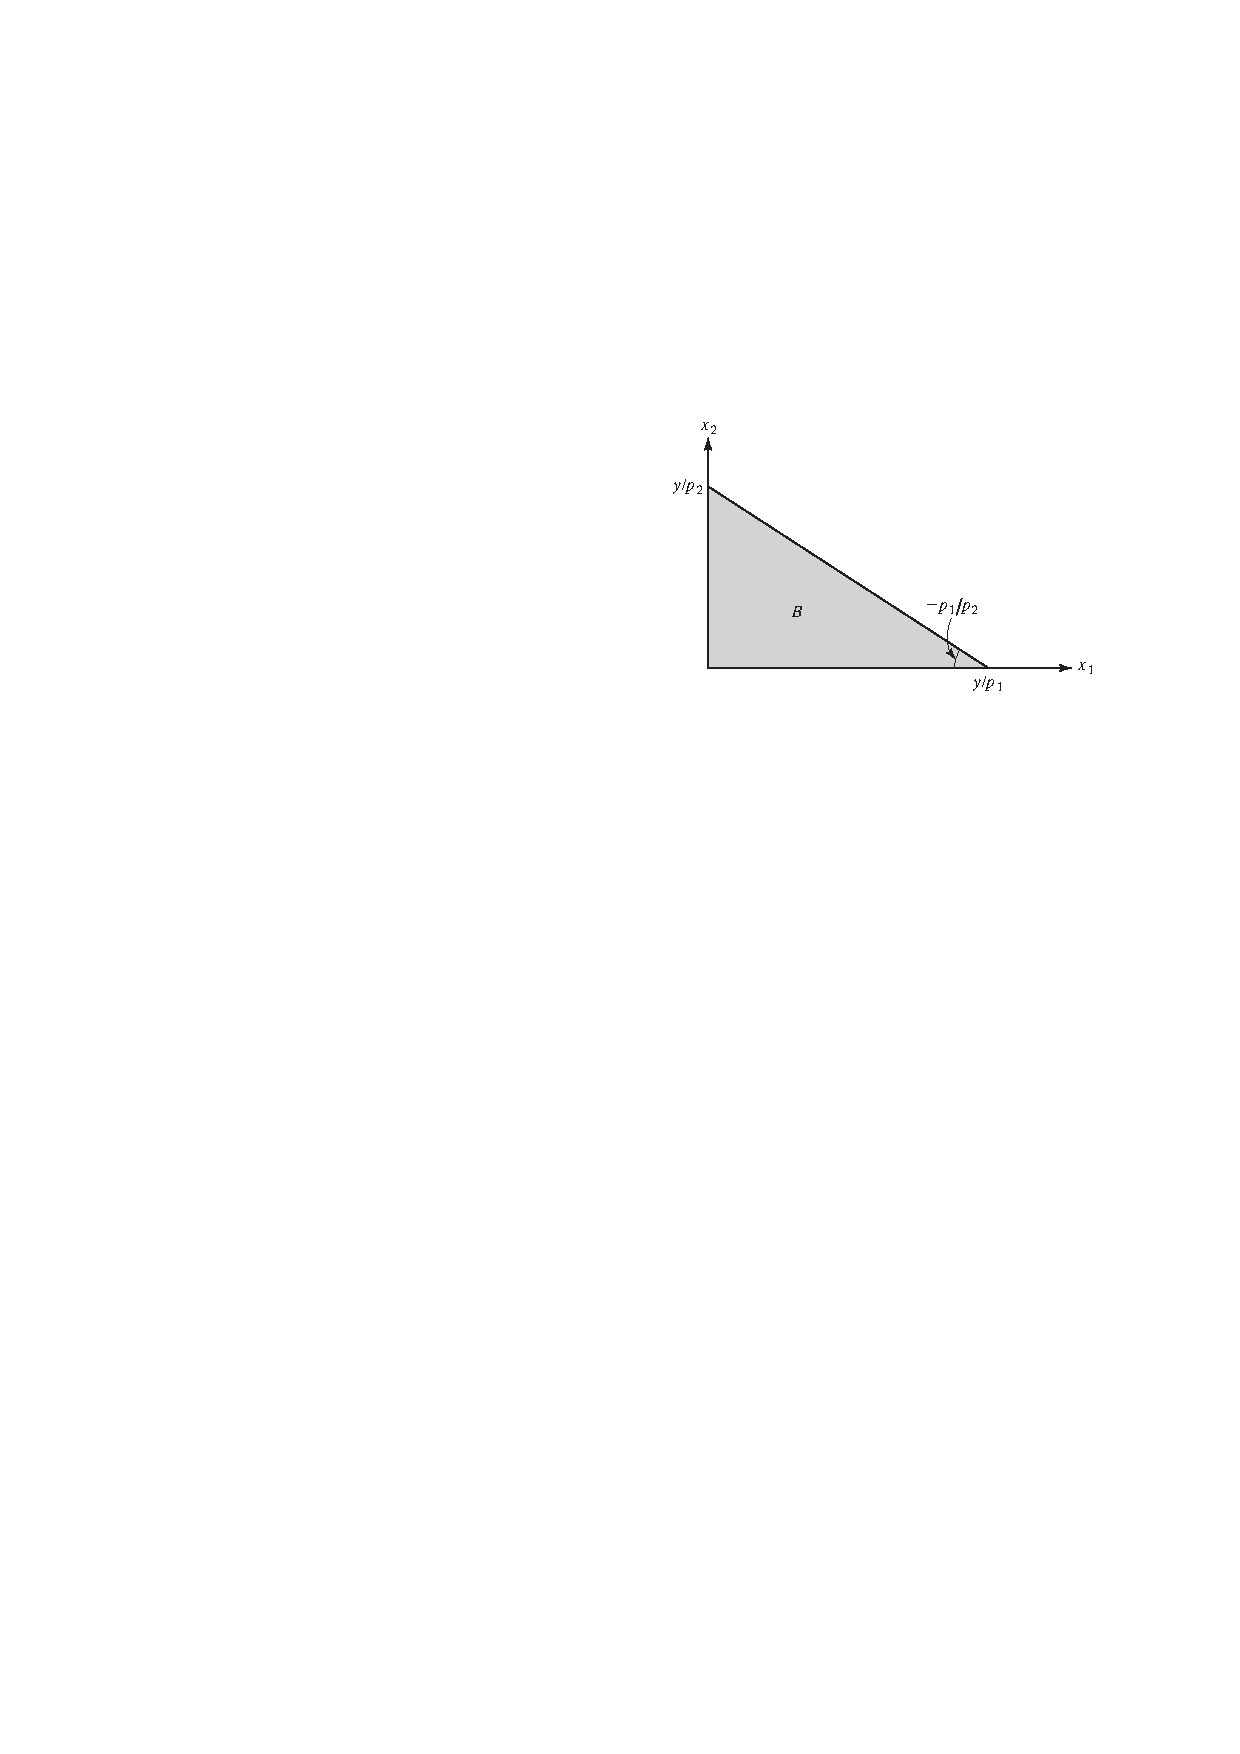
\includegraphics[width=9cm]{fig1-7.pdf}
  \caption{两种商品时的预算集$B=\{(x_1,x_2): p_1x_1+p_2x_2\leq y\}$.}\label{fig1.7}
\end{figure}

消费者的问题是在预算集$B$中选择一个消费束$\x^\ast$, 使得对于一切$\x\in B$都有$\x^\ast\succsim \x$. 在假设\ref{pos:pos1.2}成立的条件下, 该问题等价于预算约束下的\textbf{效用最大化问题} (Utility Maximization Problem, UMP)
\begin{equation}\label{eq1.3}
  \max_{\x\in\R^n_+} u(\x)\quad \text{s.t.}\quad \p\cdot\x\leq y
\end{equation}
\begin{proposition}\label{pro:pro1.2}
在假设\ref{pos:pos1.2}成立的条件下, UMP具有唯一解.
\end{proposition}
\begin{proof}
  假设$\p\gg\mathbf{0}$, 由于$B$是$\R^n_+$中的有界闭集, 根据Heine-Borel定理可知$B=\{\x\in\R_+^n:\p\cdot\x\leq y\}$是一个紧集, 由于$u$是连续函数, 故而$u$在$B$上具有最大值, 将最大值点记为$\x^\ast$, 假设还存在$\x^0\neq \x^\ast$为UMP的解, 根据$u$的严格拟凹性可知, 对于任意$t\in [0,1]$, 存在$\x^1=t\x^\ast+(1-t)\x^0$, 使得$u(\x^1)>u(\x^\ast)$, 这与$\x^\ast$为UMP的解矛盾, 因此$\x^\ast$是唯一的.
\end{proof}
根据命题\ref{pro:pro1.2}可知, 一旦给定了价格向量$\p$和财富水平$y$, UMP的解向量$\x^\ast$是唯一的, 可以用图\ref{fig1.8}表示.
\begin{figure}[htbp!]
  \centering
  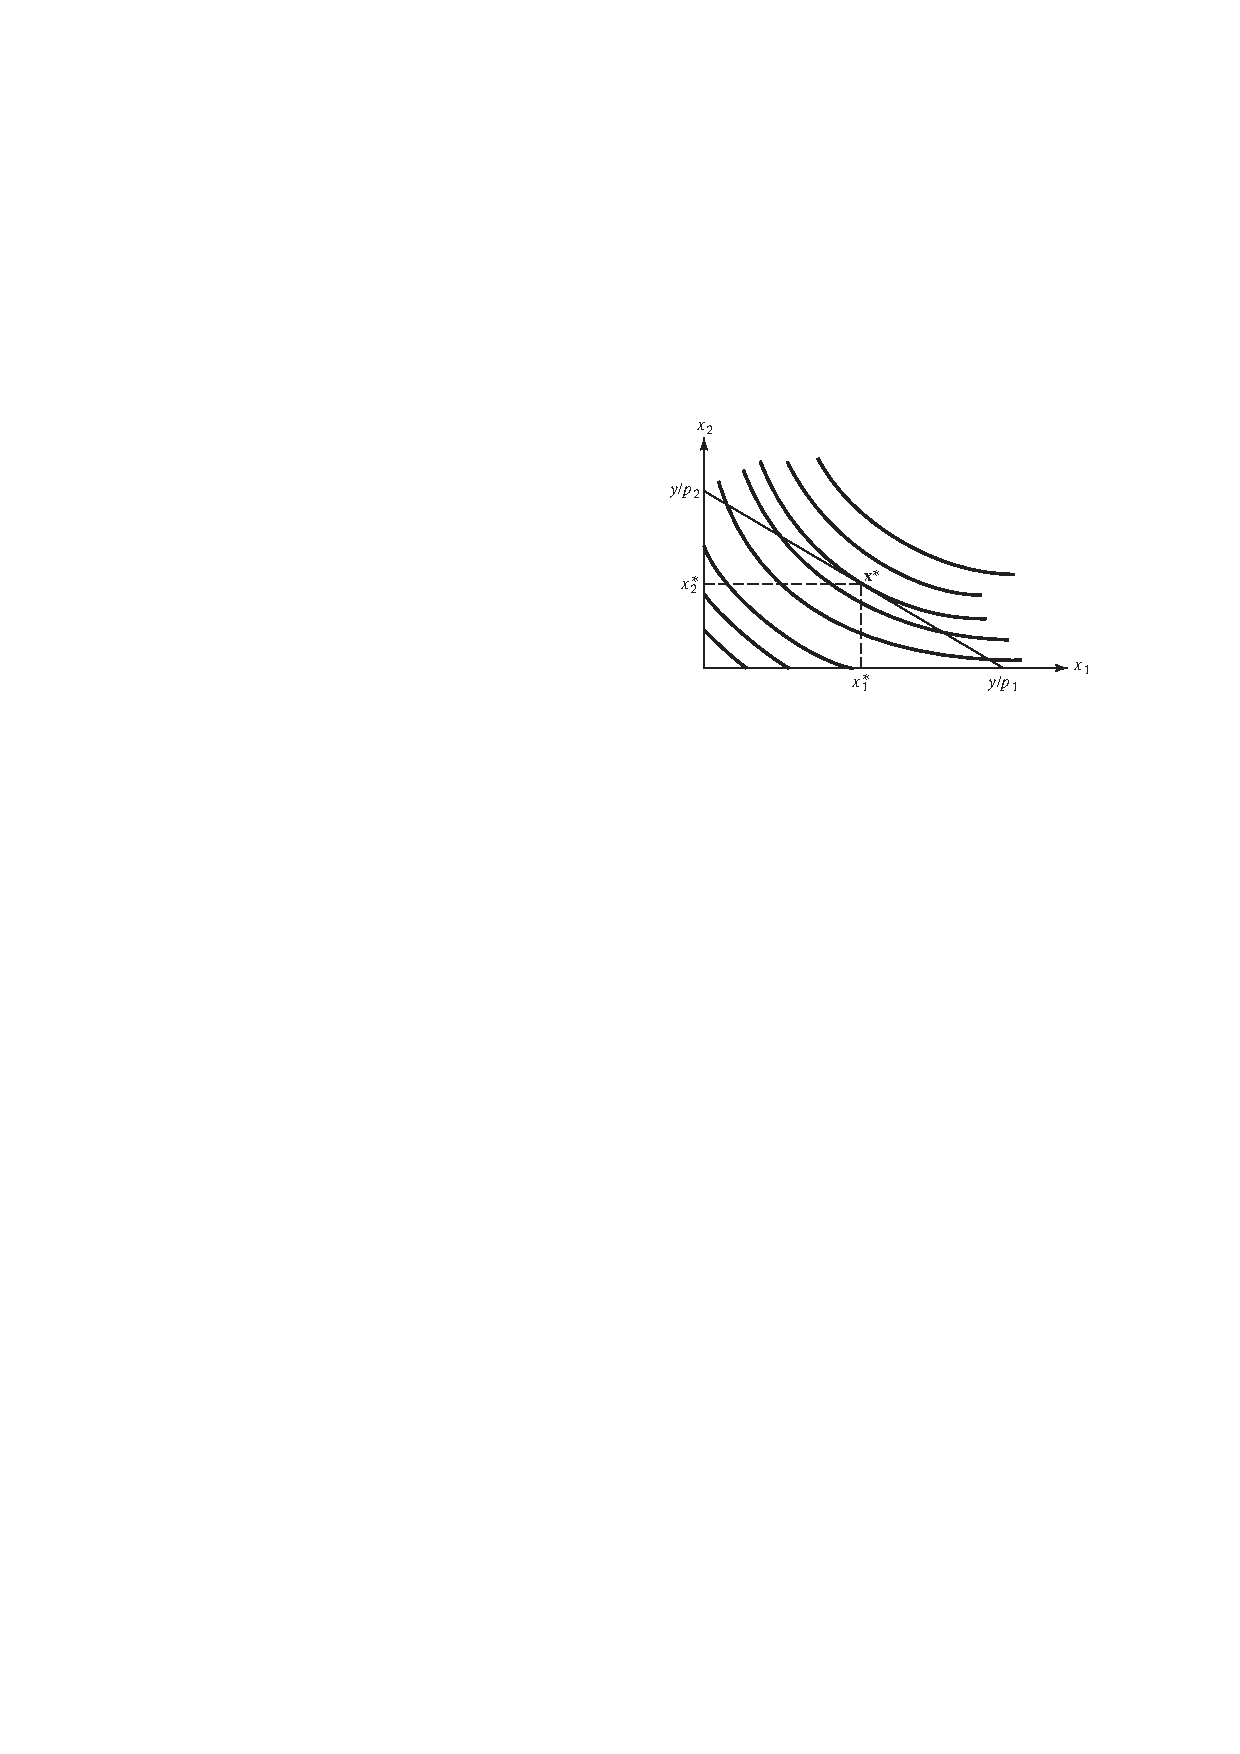
\includegraphics[width=10cm]{fig1-8.pdf}
  \caption{UMP的唯一解$\x^\ast$.}\label{fig1.8}
\end{figure}

另一方面, 可以将解向量记作$\x^\ast=\x(\p,y)$. 对于每个$i=1,\cdots,n$, 称$x_i^\ast=x_i(\p,y)$为Marshall需求函数. 当收入和其他商品的价格维持不变, 只有某商品自身的价格变化时, 需求量$x_i$和它自身价格$p_i$的关系图称为商品$i$的标准需求曲线. 特别地, 当只有两种商品时, 需求曲线如图\ref{fig1.9}所示: 保持商品2的价格$p_2^0$和收入水平$y$不变, 当商品1的价格从$p_1^0$下降至$p_1^1$时, 商品1的需求从$x_1(p_1^0,p_2^0,y)$上升至$x_1(p_1^1,p_2^0,y)$.
\begin{figure}[htbp!]
  \centering
  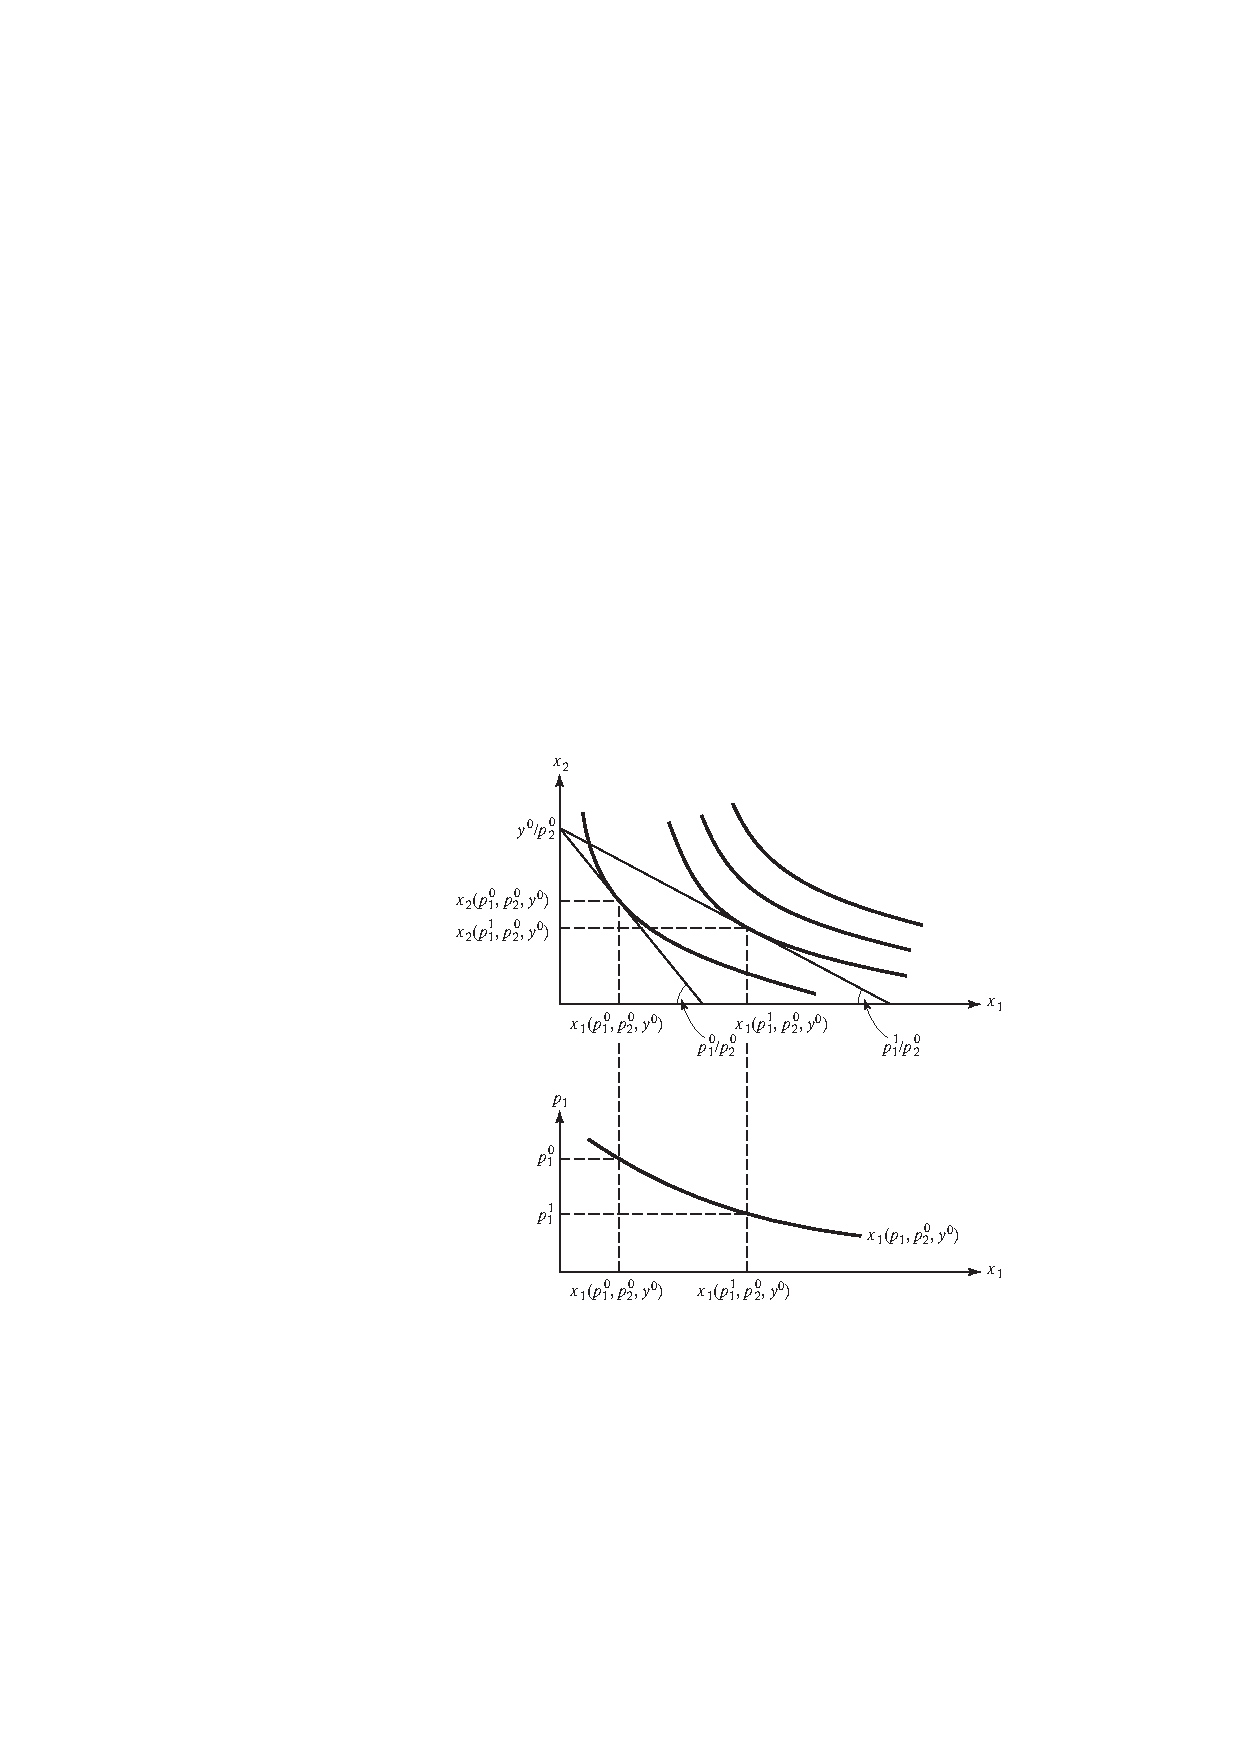
\includegraphics[width=12cm]{fig1-9.pdf}
  \caption{消费者需求行为.}\label{fig1.9}
\end{figure}

现在假设效用函数$u$是可微的, 回忆UMP为
\begin{equation}\label{eq1.4}
  \max_{\x\in\R^n_+} u(\x)\quad \text{s.t.}\quad \p\cdot\x\leq y
\end{equation}
前面已经指出UMP具有唯一解$\x^\ast$, 将约束条件改写为$\p\cdot\x\leq y$并构造Lagrange函数
$$\mathcal{L}(\x,\lambda)=u(\x)-\lambda(\p\cdot\x-y)$$
其中$\lambda$为 Lagrange乘子. 如果UMP最优解$\x^\ast\gg\mathbf{0}$, 根据Kuhn-Tucker条件可知存在$\lambda^\ast\ge0$使得$(\x^\ast,\lambda^\ast)$满足
\begin{align}
\frac{\partial\mathcal{L}}{\partial x_i}=\frac{\partial u(\x^\ast)}{\partial x_i}-\lambda^\ast p_i&=0,\,\quad i=1,\cdots, n \label{eq1.5} \\
\p\cdot\x^\ast&\leq 0  \label{eq1.6} \\
\lambda^\ast(\p\cdot\x^\ast-y)&=0 \label{eq1.7}
\end{align}
根据严格单调性可知, 为了实现消费者效用最大化, 消费者会花光全部预算$y$, 也即$\p\cdot\x^\ast=y$, 因此式(\ref{eq1.7})是多余的. 此时, 上述条件可以简化为
\begin{align}
\begin{split}
\frac{\partial\mathcal{L}}{\partial x_1}=\frac{\partial u(\x^\ast)}{\partial x_1}-\lambda^\ast p_1&=0  \\
&\vdots  \\
\frac{\partial\mathcal{L}}{\partial x_n}=\frac{\partial u(\x^\ast)}{\partial x_n}-\lambda^\ast p_n&=0 \\
\p\cdot\x^\ast&=0
\end{split}
\label{eq1.8}
\end{align}
假设$\nabla u(\x^\ast)=\mathbf{0}$, 由严格单调性可知$\partial u(\x^\ast)/\partial x_i>0$, $i=1,\cdots,n$, 从而$\partial u(\x^\ast)/\partial x_i=\lambda^\ast p_i>0$. 由此可见, 对于任意商品$i$和$j$, 在UMP的解$\x^\ast$处有
\begin{equation}\label{eq1.9}
  \text{MRS}_{ij}(\x^\ast)=\frac{\partial u(\x^\ast)/\partial x_j}{\partial u(\x^\ast)/\partial x_i}=\frac{p_j}{p_i}
\end{equation}
表明最优解$\x^\ast$处的两种商品的边际替代率必然等于这两种商品价格之比.

一般而言, 式(\ref{eq1.8})表示的一阶条件 (First Order Condition, FOC)只是局部最优解的必要条件, 但以下定理表明, FOC也是UMP全局最优解的充分条件.

\begin{theorem}\label{thm:thm1.7}
  设$u$在$\R_+^n$是连续和拟凹的, 并且$(\p,y)\gg\mathbf{0}$, 如果$u$在$\x^\ast$处可微并且$(\x^\ast,\lambda^\ast)$是方程组(\ref{eq1.8})的解, 那么$\x^\ast$也是UMP在$(\p,y)$时的解.
\end{theorem}
\begin{proof}
  假设$\nabla u(\x^\ast)$存在且$(\x^\ast,\lambda^\ast)$是方程组(\ref{eq1.8})的解, 那么
  \begin{align*}
  \nabla u(\x^\ast)&=\lambda^\ast\p \\
  \p\cdot\x^\ast&=y
  \end{align*}
  如果$\x^\ast$不是UMP的解, 那么必然存在某个$\x^0\in \R^n_+$, 使得
  \begin{align*}
  u(\x^0)&=u(\x^\ast) \\
  \p\cdot\x^0&\leq y
  \end{align*}
  由于$u$是连续函数且$y>0$, 于是存在某个充分接近1的实数$t\in [0,1]$, 使得
  \begin{align*}
  u(t\x^0)&>u(\x^\ast) \\
  \p\cdot t\x^0&<y
  \end{align*}
  再令$\x^1=t\x^0$, 于是
  $$\nabla u(\x^\ast)(\x^1-\x^\ast)=(\lambda^\ast\p)\cdot(\x^1-\x^\ast)=\lambda^\ast(\p\cdot\x^1-\p\cdot\x^\ast)<\lambda^\ast(y-y)=0$$
  由于$u$是拟凹的且$u(\x^1)\geq u(\x^\ast)$, 于是对于任意$t\in[0,1]$都有
  $$\frac{u(t(\x^1-\x^\ast)+\x^\ast)-u(\x^\ast)}{t}\ge0$$
  当$t\to0$时取极限可得$\nabla u(\x^\ast)(\x^1-\x^\ast)\ge 0$
  这就产生了矛盾, 因此$\x^\ast$必然是UMP的解.
\end{proof}
\begin{example}
设$u(x_1,x_2)=(x_1^\rho+x_2^\rho)^{1/\rho}$, $0\ne \rho<1$, 称为CES效用函数, 容易证明它代表的偏好是严格单调和严格凸的. 考虑消费者问题
\begin{equation}\label{eq1.10}
  \max_{x_1,x_2}(x_1^\rho+x_2^\rho)^{1/\rho}\quad \text{s.t.}\quad p_1x_1+p_2x_2\leq y
\end{equation}
构造Lagrange函数
$$\mathcal{L}(x_1,x_2,\lambda)=(x_1^\rho+x_2^\rho)^{1/\rho}-\lambda(p_1x_1+p_2x_2-y)$$
得到FOC为
\begin{align*}
\frac{\partial \mathcal{L}}{\partial x_1}&=(x_1^\rho+x_2^\rho)^{1/\rho}x_1\rho^{\rho-1}-\lambda p_1=0 \\
\frac{\partial \mathcal{L}}{\partial x_2}&=(x_1^\rho+x_2^\rho)^{1/\rho}x_2\rho^{\rho-1}-\lambda p_2=0 \\
\frac{\partial \mathcal{L}}{\partial \lambda}&=p_1x_1+p_2x_2-y=0
\end{align*}
求得UMP (\ref{eq1.10})的最优解为
\begin{align*}
x_1(p_1,p_2,y)&=\frac{p_1^{r-1}y}{p_1^r+p_2^r} \\
x_2(p_1,p_2,y)&=\frac{p_2^{r-1}y}{p_1^r+p_2^r}
\end{align*}
其中$r=\rho/(\rho-1)$.
\end{example}

\section{间接效用函数与支出}
\subsection{间接效用函数}
上面已经指出$u(\x)$是定义在消费集$X$上表示偏好关系$\succsim$的效用函数, 更具体地称为\textbf{直接效用函数} (direct utility function). 给定价格向量$\p$和收入水平$y$, 消费者选择效用最大化的商品束$\x(\p,y)$, 当$\p$和$y$发生变动时, $u(\x)$的最大值也发生变动, 这可以用函数关系$v:\R_{++}^n\times \R_+\to \R$表示, $v$的定义如下
\begin{equation}\label{eq1.11}
  v(\p,y)=\max_{x\in\R_+^n}u(\x)\quad\text{s.t.}\quad\p\cdot\x\leq y
\end{equation}
称$v$为\textbf{间接效用函数} (indirect utility function), 它是UMP对应的效用最大值函数.

当$\p\gg\mathbf{0}$和$y>0$时, $v(\p,y)$是具有良好定义的函数, 因为问题(\ref{eq1.11})的解确实存在. 如果$u(\x)$是严格拟凹的, 则该问题的解唯一, 将其记作$\x(\p,y)$, 此时
$$v(\p,y)=u(\x(\p,y))$$
如图\ref{fig1.10}所示, 可以把$v(\p,y)$视作当$\p$和$y$给定时, 消费者能达到的最高无差异曲线所代表的效用水平.
\begin{figure}[htbp!]
  \centering
  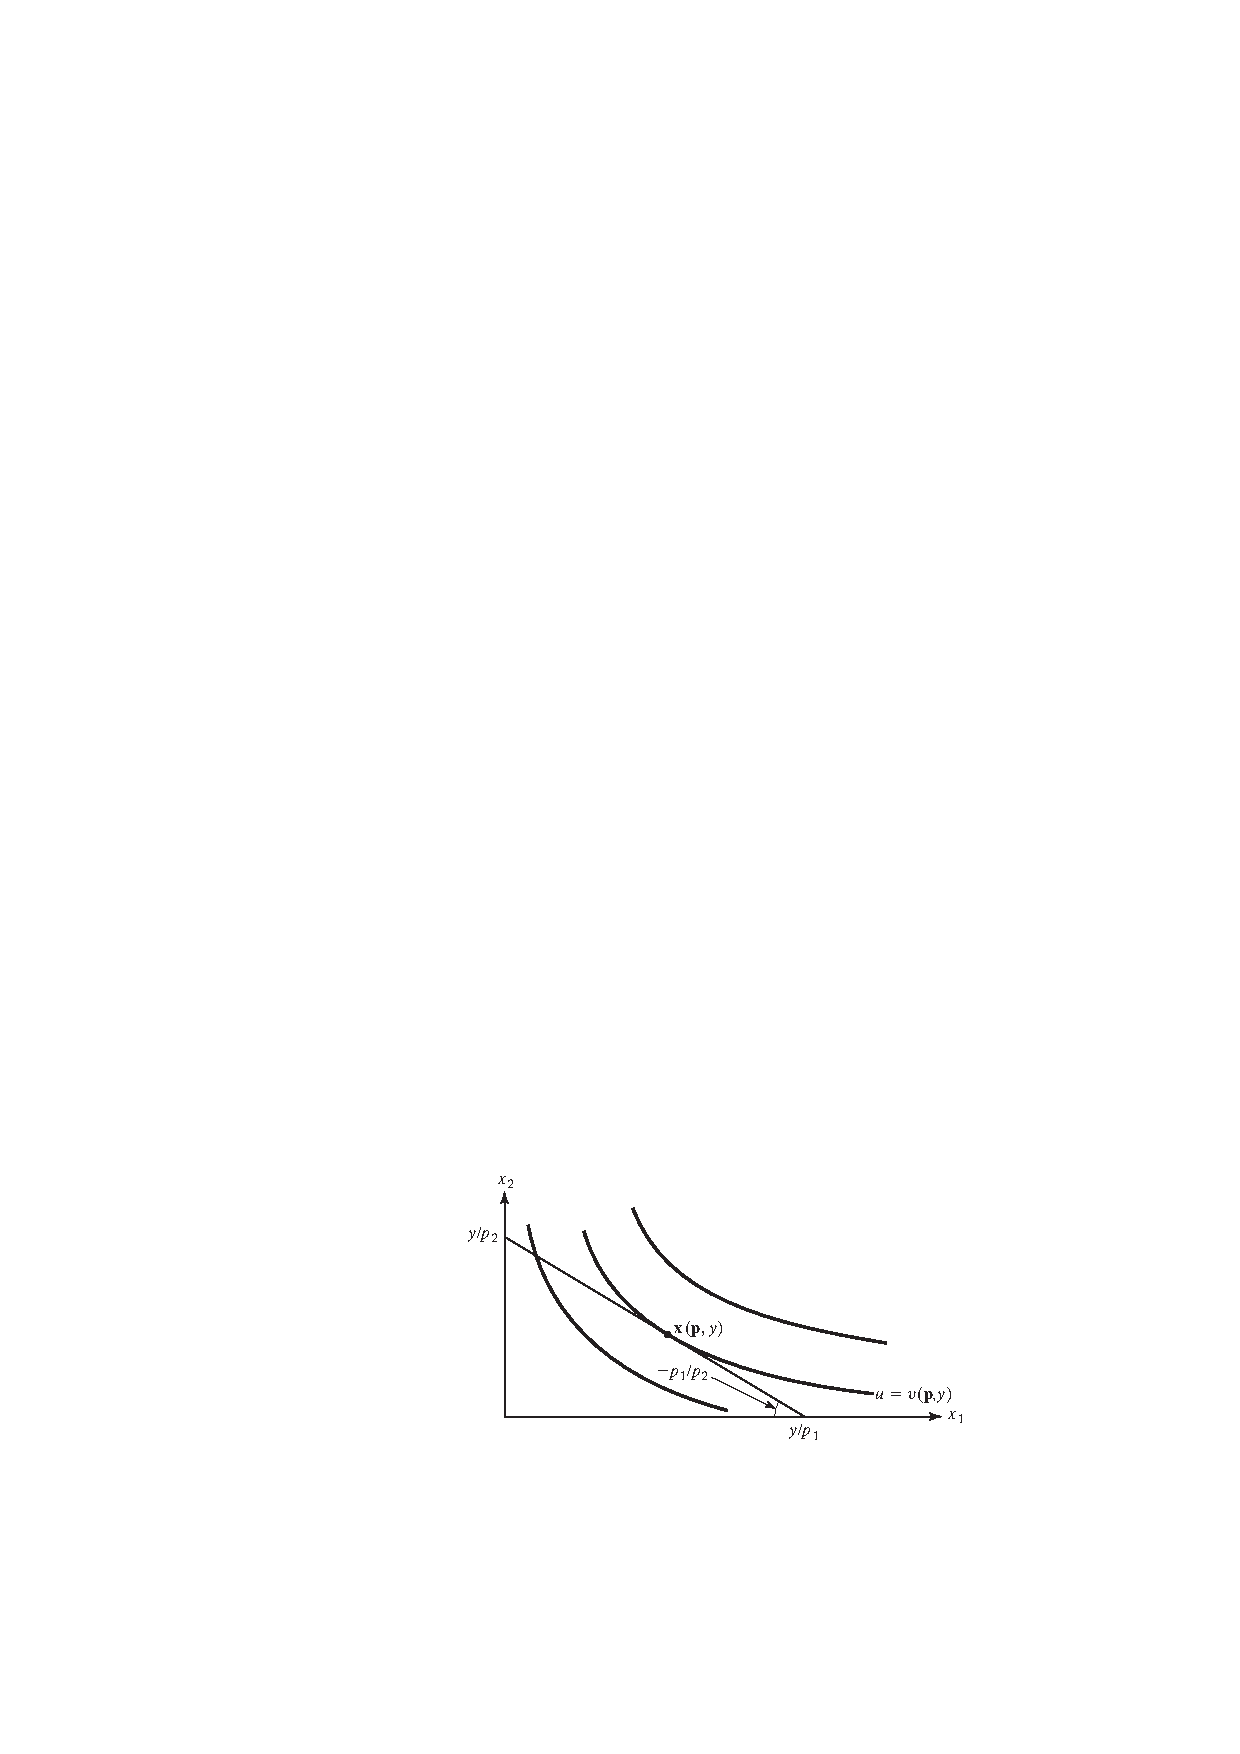
\includegraphics[width=10cm]{fig1-10.pdf}
  \caption{价格为$\p$收入为$y$时的间接效用函数$v(\p,y)$.}\label{fig1.10}
\end{figure}
\begin{theorem}[间接效用函数的性质]
  如果$u$在$\R_+^n$上连续且严格递增, 那么间接效用函数$v(\p,y)$具有以下性质:
  \begin{enumerate}[label=\arabic*.]
    \item 在$\R_{++}^n\times\R_+$上连续;
    \item 关于$(\p,y)$是零次齐次的;
    \item 关于$\p$是递减的;
    \item 关于$y$是递增的;
    \item 关于$(\p,y)$是拟凸的.
  \end{enumerate}
\end{theorem}
\begin{proof}
  1. 略.

  2. 对于任意$t>0$, 以下问题
  $$v(t\p,ty)=\max_{x\in\R_+^n}u(\x)\quad\text{s.t.}\quad t\p\cdot\x\leq y$$
  等价于问题(\ref{eq1.11}), 因此$v(t\p,ty)=v(\p,y)$对于$t>0$恒成立.

  3. 设$\p^0\ge\p^1$, $\x^0$是$\p=\p^0$时问题(\ref{eq1.11})的解, 因为$u$是严格递增的, 故而偏好关系$\succsim$是严格单调的, 此时约束条件变为$\p^0\cdot\x^0=y$, 故而$\p^1\cdot\x^0\leq y$, 此时消费者必然选择最优消费束$\x^1\ge \x^0$使得$\p^1\cdot\x^1=y$, 因此$v(\p^1,y)=u(\x^1)\geq u(\x^0)=v(\p^0,y)$.

  4. 设$y^0\ge y^1$, $\x^0$是$y=y^0$时问题(\ref{eq1.11})的解, 同上可知当价格水平$\p$不变时, 随着收入水平的下降, 消费者为实现$\p\cdot\x=y$, 只能将消费束缩减为$\x^1\leq \x^0$, 于是$v(\p,y^1)=u(\x^1)\leq u(\x^0)=v(\p,y^0)$.

  5. 只需证明$v$的下轮廓集$\{(\p,y):v(\p,y)\leq q\}$对于任意$q\in\R$都是凸的. 假设对于$(\p^0,y^0)$和$(\p^1,y^1)$都有$v(\p^0,y^0)\leq q$及$v(\p^1,y^1)\leq q$, 对于任意$t\in[0,1]$, 定义
  \begin{align*}
  \p^2&=t\p^0+(1-t)\p^1 \\
  y^2&=ty^0+(1-t)y^1
  \end{align*}
  现在需要证明$v(\p^2,y^2)\leq q$. 由于$v(\p^2,y^2)$是价格为$\p^2$且收入为$y^2$时$u(\x)$的最大值函数, 故而只需证明此时对一切$\x\in\R_+^n$都有$u(\x)\leq q$即可. 注意到如果$\p^2\cdot\x\leq y^2$, 那么
  $$t\p^0\cdot\x+(1-t)\p^1\cdot\x\leq ty^0+(1-t)y^1$$
  因此, 要么$\p^0\cdot \x\leq y^0$, 要么$\p^1\cdot\x\leq y^1$, 或者两者都成立. 如果$\p^0\cdot \x\leq y^0$, 那么$u(\x)\leq v(\p^0,y^0)\leq q$; 如果$\p^1\cdot\x\leq y^1$, 那么$u(\x)\leq v(\p^1,y^1)\leq q$, 结论成立.

\end{proof}
\begin{theorem}[Roy恒等式]
  如果$u$在$\R_+^n$上连续且严格递增, $v$在$(\p^0,y^0)\gg\mathbf{0}$处可微且$\partial v(\p^0,y^0)/\partial y\ne0$, 那么
  $$x_i(\p^0,y^0)=-\frac{\partial v(\p^0,y^0)/\partial p_i}{\partial v(\p^0,y^0)/\partial y},\quad i=1,\cdots,n$$
\end{theorem}
\begin{proof}
  假设$\x^0=\x(\p^0,y^0)$, 再定义$v(\p,\p\cdot\x^0)$, 于是
  $$v(\p,\p\cdot\x^0)=\max_{\x\in\R_+^n}u(\x)\quad\text{s.t.}\quad \p\cdot\x\leq \p\cdot\x^0$$
  由于$\x^0$位于预算集内, 故而$v(\p,\p\cdot\x^0)\geq u(\x^0)=v(\p^0,\p^0\cdot\x^0)$对任意$\p\gg\mathbf{0}$成立. 再定义函数$f(\p)=v(\p,\p\cdot\x^0)$, 显然当$\p=\p^0$时, $f(\p)$在$\R_{++}^n$内取得最小值, 由于$v$在$(\p^0,y^0)$处可微, 故而$f$在$\p=\p^0$处的梯度为$\mathbf{0}$, 因此
  $$\frac{\partial f(\p^0)}{\partial \p}=\frac{\partial v(\p^0,\p^0\cdot\x^0)}{\partial \p}+\frac{\partial v(\p^0,\p^0\cdot\x^0)}{\partial (\p\cdot\x^0)}\x^0=\mathbf{0}$$
  整理即得结论.
\end{proof}
值得注意的是, 如果问题(\ref{eq1.11})的解$\x^\ast=\x(\p,y)$严格为正并且是可微的, 那么此时可以定义Lagrange函数
$$\mathcal{L}(\x,\lambda;\p,y)=u(\x)-\lambda(\p\cdot\x-y)$$
于是$v(\p,y)$是$\mathcal{L}(\x,\lambda;\p,y)$的最优值函数, 根据\textbf{包络定理} (envelope theorem)可知在最优解$(\x^\ast,\lambda^\ast)$处有
$$\frac{\partial v(\p,y)}{\partial p_i}=\frac{\partial \mathcal{L}}{\partial p_i}=-\lambda^\ast x_i^\ast$$
以及
$$\frac{\partial v(\p,y)}{\partial y}=\frac{\partial \mathcal{L}}{\partial y}=\lambda^\ast$$
结合以上二式即可推得Roy恒等式.

\begin{example}
考虑CES效用函数$u(x_1,x_2)=(x_1^\rho+x_2^\rho)^{1/\rho}$, $0\neq\rho<1$, 于是Marshall需求函数为
$$x_1(\p,y)=\frac{p_1^{r-1}y}{p_1^r+p_2^r},\quad x_2(\p,y)=\frac{p_2^{r-1}y}{p_1^r+p_2^r}$$
其中$r=\rho/(\rho-1)$. 进一步可得间接效用函数
$$v(\p,y)=\{[x_1(\p,y)]^\rho+[x_2(\p,y)]^\rho\}^{1/\rho}=y(p_1^r+p_2^r)^{-1/r}$$
\end{example}
\subsection{支出函数}
现在我们想知道给定一组价格, 消费者能够实现既定效用水平的最小货币支出水平为多少, 如图\ref{fig1.11}所示, 预算约束线从东北往西南移动的过程中, 消费者可以选取无差异曲线上的消费束以实现既定效用水平$u$, 直观上看, 最低的预算约束线是和无差异曲线相切的那条.

事实上, 图\ref{fig1.11}中平行的\textbf{等支出线 }(isoexpenditure curve)$e=p_1x_1+p_2x_2$描述的是价格水平$\p=(p_1,p_2)$保持不变时, 在各收入水平下消费的商品束. 当支出水平低至$e^3$时, 显然消费者无法实现效用水平$u$.

\begin{figure}[htbp!]
  \centering
  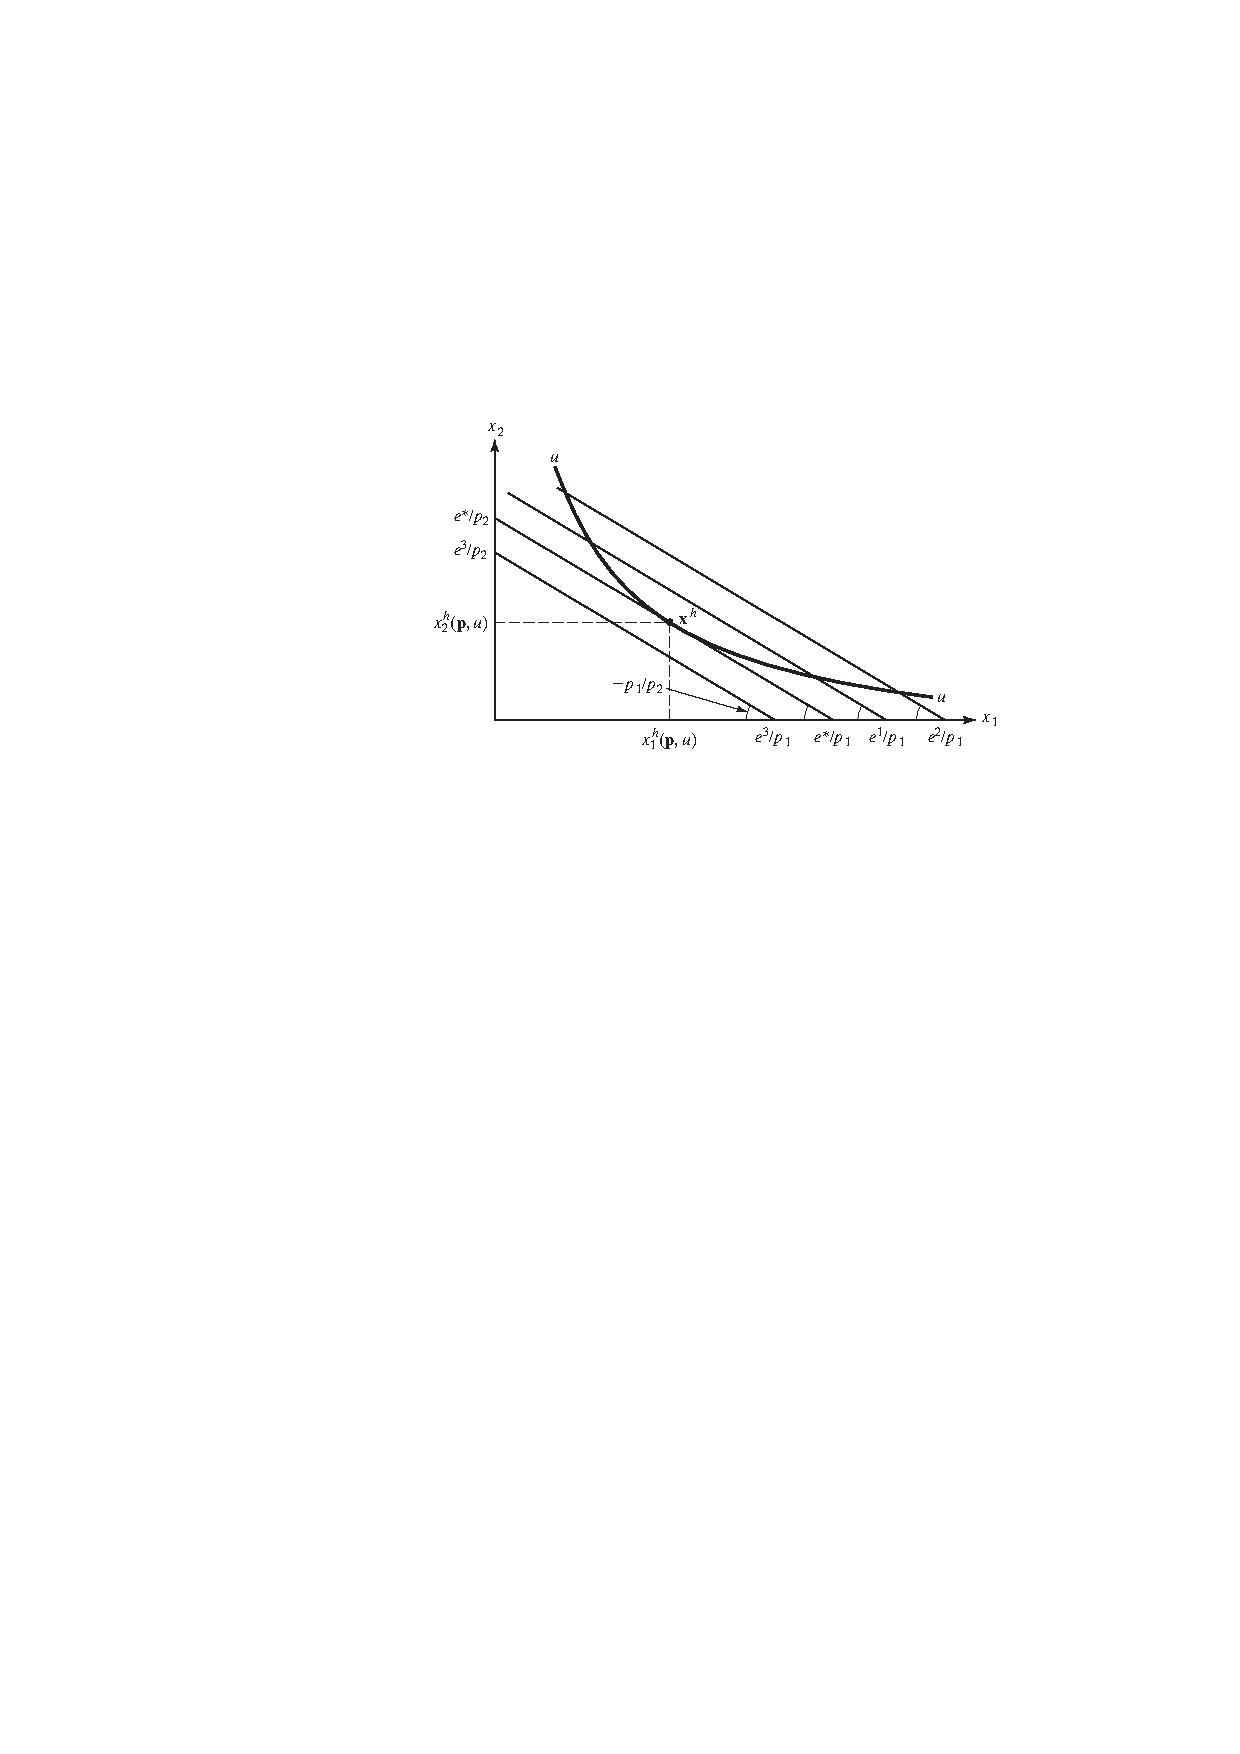
\includegraphics[width=10cm]{fig1-11.pdf}
  \caption{寻找最低预算水平使得消费者达到既定效用水平$u$.}\label{fig1.11}
\end{figure}

更一般地, 考虑将消费者\textbf{支出最小化问题} (Expenditure Minimization Problem, EMP)定义为
\begin{equation}\label{eq1.12}
  e(\p,u)=\min_{\x\in\R_+^n} \p\cdot\x\quad\text{s.t.}\quad u(\x)\ge u
\end{equation}
其中$e(\p,u)$称为\textbf{支出函数} (expenditure function), 方便起见, 定义$\mathcal{U}=\{u(\x):\x\in\R_+^n\}$表示可以达到的效用水平, 支出函数$e$的定义域为$\R_{++}^n\times\mathcal{U}$.

支出函数$e(\p,u)$的定义是良好的, 这是因为对于任意$\p\gg\mathbf{0}$和$\x\in\R_+^n$, 集合$\{e=\p\cdot\x: u(\x)\geq u\}$存在下界0, 还可以证明它是闭集, 因而它有最小值, 这个最小值就是$e(\p,u)$.

EMP的任意解向量都非负且取决于$(\p,u)$, 如果效用函数$u$是连续和严格拟凹的, 那么解唯一. 如果$\x^h(\p,u)$是EMP的解, 那么它表示价格水平为$\p$时, 为使消费者达到效用水平$u$的最小支出恰好等于消费商品束$\x^h(\p,u)$的支出, 也即$e(\p,u)=\p\cdot\x^h(\p,u)$. 事实上, 对于特定的商品$i$而言, $x_i^h(\p,u)$又称为Hicks需求函数或补偿需求函数.

如图\ref{fig1.12}所示, 维持商品2的价格$p_2^0$不变, 当商品1的价格从$p_1^0$下降到$p_1^1$时, 为使消费者获得相同的效用$u$且实现最小支出, 应将等支出线沿着它和无差异曲线的切点移动, 此时商品1的消费量从$x_1^h(p_1^0,p_2^0,u)$上升为$x_1^h(p_1^1,p_2^0,u)$, 这样一直做下去即可得到商品1的Hicks需求曲线. 显然, 效用水平不同Hicks需求曲线也不同, 但它的形状和位置总取决于消费者的偏好.
\begin{figure}[htbp!]
  \centering
  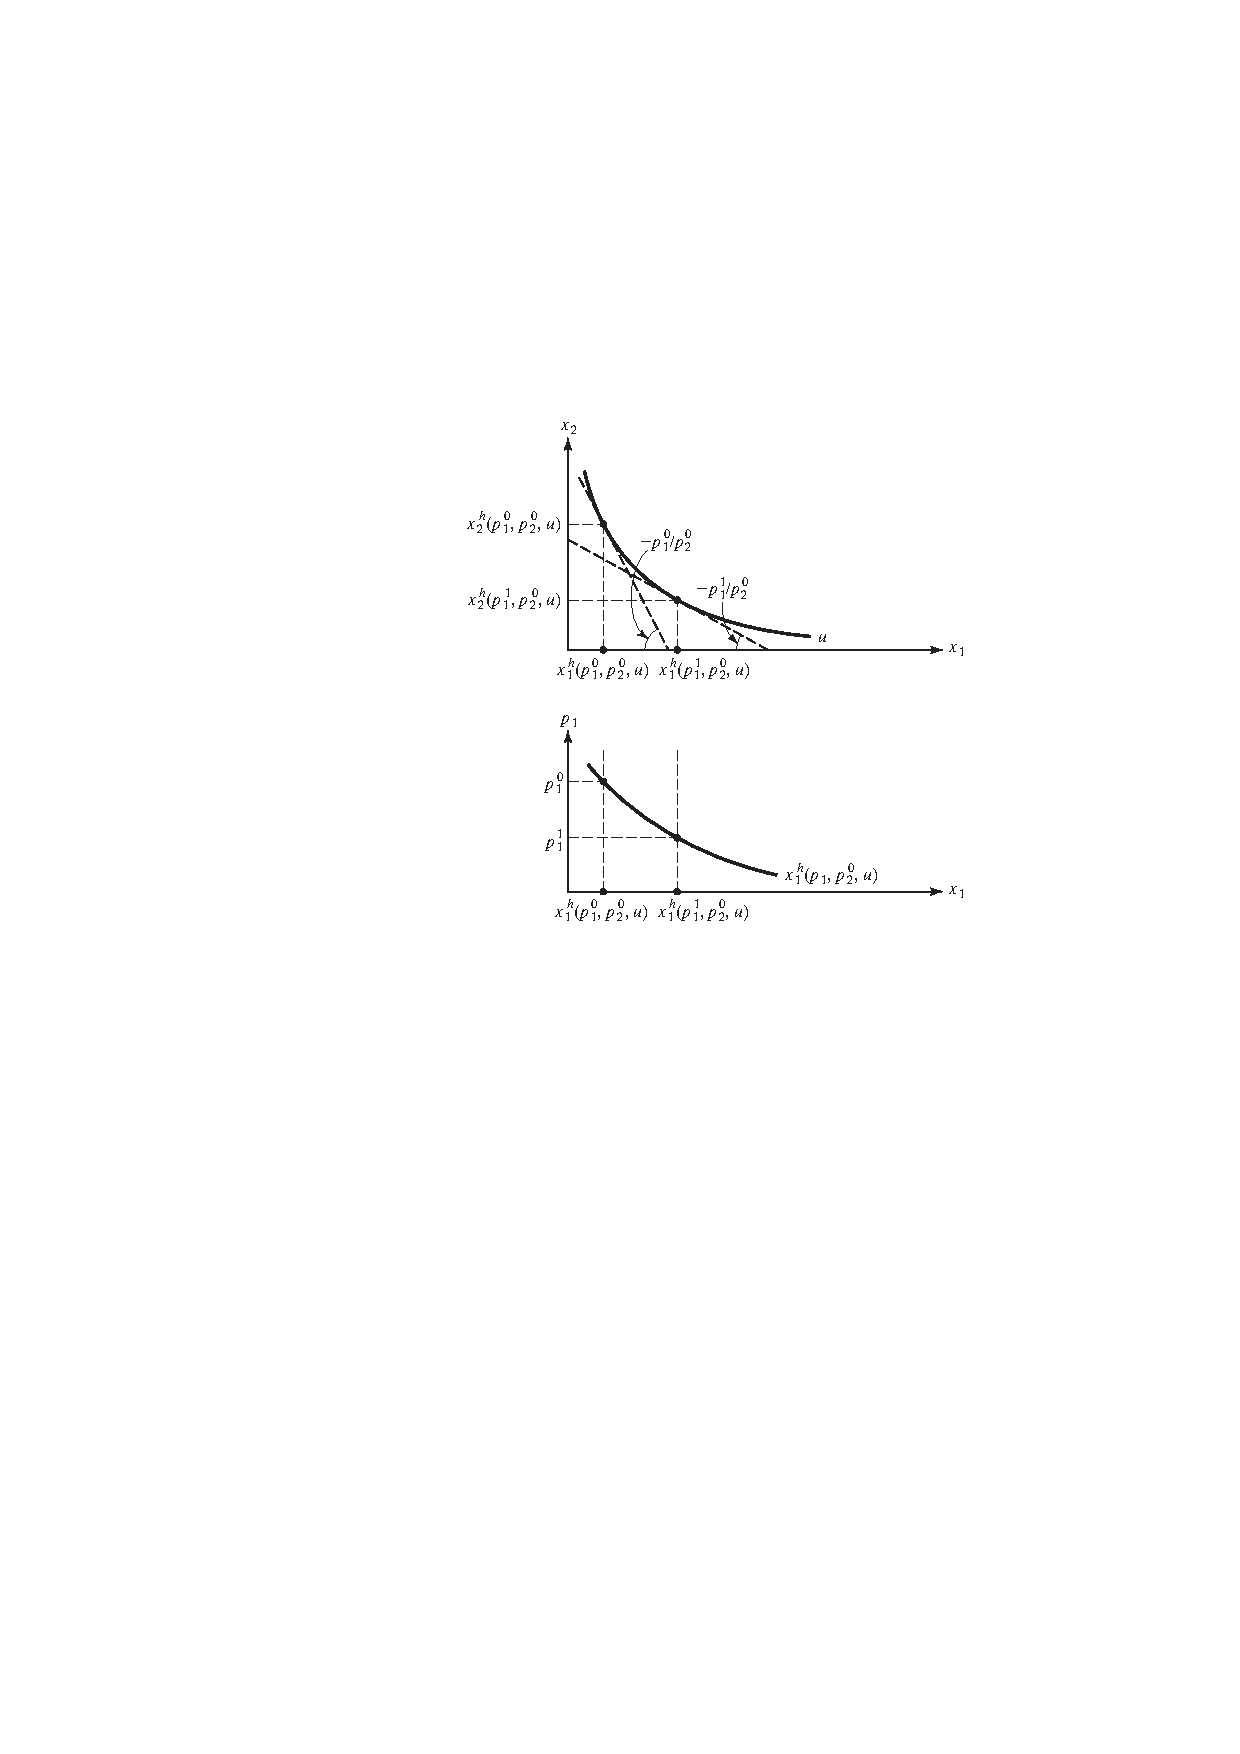
\includegraphics[width=10cm]{fig1-12.pdf}
  \caption{商品1的Hicks需求函数.}\label{fig1.12}
\end{figure}

\begin{theorem}[支出函数的性质]\label{thm:thm1.6}
  如果$u$在$\R_+^n$上连续且严格递增, 那么支出函数$e(\p,u)$具有以下性质:
  \begin{enumerate}[label=\arabic*.]
    \item 在$\R_{++}^n\times\mathcal{U}$上连续;
    \item 关于$u$是递增的且无上界;
    \item 关于$\p$是递增的;
    \item 关于$\p$是一次齐次的;
    \item 关于$\p$是凹函数.
  \end{enumerate}
\end{theorem}
\begin{proof}
  1. 略.

  2. 假设$e$关于$u$不是递增的, 设$\x^0$和$\x^1$分别为效用水平为$u^0$和$u^1$时的最优消费束, 并且$u^1>u^0$, $\p\cdot\x^0\geq \p\cdot\x^1>0$. 设$t\in[0,1]$为充分接近1的某个数, $\x^2=t\x^1$, 由于效用函数$u$是连续的, 故而$u(\x^2)>u^0$且$\p\cdot\x^0>\p\cdot\x^2$, 但这与$\x^0$是既定效用水平为$u^0$时的最优消费束这一事实矛盾.

  由于$u$在$\R_+^n$上连续且严格递增, 当$u(\x)\to \infty$时, $\x$中至少有一个分量趋近于$\infty$, 因此$\min \p\cdot\x$也是如此.

  3. 假设$\p^0\ge\p^1$, $\x^0$是价格为$\p^0$时EMP的最优解, 于是
  $$e(\p^0,u)=\p^0\cdot\x^0\ge \p^1\cdot\x^0\ge e(\p^1,u)$$
  其中最后一个不等号是由$e(\p^1,u)$的定义得到的.

  4. 当价格变化时, EMP的约束集不会发生变化, 对于任意$t\ge0$, 在约束集上使$t\p\cdot\x$最小化的消费束和使$\p\cdot\x$最小化的消费束是一致的, 将其记作$\x^\ast$, 于是$e(t\p,u)=t\p\cdot\x^\ast=te(\p,u)$.

  5. 固定目标效用水平$u$, 对任意$t\in(0,1)$, 定义$\p^2=t\p^0+(1-t)\p^1$, $\x^2$是价格为$\p^2$时的EMP最优消费束, 于是
  \begin{align*}
  e(\p^2,u)&=\p^2\cdot\x^2 \\
  &=t\p^0\cdot\x^2+(1-t)\p^1\cdot\x^2 \\
  &\geq te(\p^0,u)+(1-t)e(\p^1,u)
  \end{align*}
  也即$e$关于$\p$是凹的.
\end{proof}

\begin{theorem}[Shephard引理]
  如果$u$在$\R_+^n$上连续且严格递增, 并且是严格拟凹的, 那么$e$在$(\p^0,u^0)$处关于$\p\gg\mathbf{0}$可微, 并且
  $$x_i^h(\p^0,u^0)=\frac{\partial e(\p^0,u^0)}{\partial p_i},\quad i=1,\cdots,n$$
\end{theorem}
\begin{proof}
  设$\p^0\gg\mathbf{0}$并且$\x^0=\x^h(\p^0,u^0)$, 于是
  $$e(\p,u^0)=\min_{\x\in\R_+^n}\p\cdot\x\quad\text{s.t.}\quad u(\x)\ge u^0$$
  也即$e(\p,u^0)$是价格为$\p$且既定效用水平为$u^0$时的最小支出, 而$\x^0=\x^h(\p^0,u^0)$也是可以实现既定效用水平$u^0$的消费束, 故而对于一切$\p\gg\mathbf{0}$都有$e(\p,u^0)\leq \p\cdot\x^0$.

  定义函数$f(\p)=e(\p,u^0)-\p\cdot\x^0$, 当且仅当$\p=\p^0$时$f$在$\R_{++}^n$上有最大值, 根据可微性可知
  $$\frac{\partial f(\p^0)}{\partial \p}=\frac{\partial e(\p^0,u^0)}{\partial \p}-\x^0=\mathbf{0}$$
  结论成立.
\end{proof}
\begin{example}
考虑CES效用函数$u(x_1,x_2)=(x_1^\rho+x_2^\rho)^{1/\rho}$, $0\neq\rho<1$, 现在来推导Hicks需求函数$\x^h(\p,u)$与支出函数$e(\p,u)$. 由于偏好关系$\succsim$是严格单调的, 故而将EMP写为
$$\min_{(x_1,x_2)\in\R_+^2}p_1x_1+p_2x_2\quad\text{s.t.}\quad u=(x_1^\rho+x_2^\rho)^{1/\rho}$$
首先定义Lagrange函数
$$\mathcal{L}(x_1,x_2,\lambda)=p_1x_1+p_2x_2-\lambda[(x_1^\rho+x_2^\rho)^{1/\rho}-u]$$
于是
\begin{align*}
\frac{\partial\mathcal{L}}{\partial x_1}&=p_1-\lambda(x_1^\rho+x_2^\rho)^{1/\rho-1}x_1^{\rho-1}=0 \\
\frac{\partial\mathcal{L}}{\partial x_2}&=p_2-\lambda(x_1^\rho+x_2^\rho)^{1/\rho-1}x_2^{\rho-1}=0 \\
\frac{\partial\mathcal{L}}{\partial\lambda}&=(x_1^\rho+x_2^\rho)^{1/\rho}-u
\end{align*}
消去$\lambda$后可得包含两个未知数的方程
\begin{align}
x_1&=x_2\left(\frac{p_1}{p_2}\right)^{1/(\rho-1)} \label{eq1.13} \\
u&=(x_1^\rho+x_2^\rho)^{1/\rho} \label{eq1.14}
\end{align}
将式(\ref{eq1.13})代入(\ref{eq1.14})得到
$$  u=\left[x_2^\rho\left(\frac{p_1}{p_2}\right)^{\rho/(\rho-1)}+x_2^\rho\right]^{1/\rho}=x_2\left[\left(\frac{p_1}{p_2}\right)^{\rho/(\rho-1)}+1\right]^{1/\rho}
$$
再令$r=\rho/(\rho-1)$, 得到
\begin{equation}\label{eq1.15}
  x_2^h(\p,u)=u(p_1^r+p_2^r)^{1/r-1}p_2^{r-1}
\end{equation}
将式(\ref{eq1.15})代入(\ref{eq1.13})得到
$$  x_1^h(\p,u)=u(p_1^r+p_2^r)^{1/r-1}p_1^{r-1}
$$
从而支出函数为
\begin{align*}
e(\p,u)&=p_1x_1^h(\p,u)+p_2x_2^h(\p,u)=u(p_1^r+p_2^r)^{1/r}
\end{align*}
\end{example}
\subsection{间接效用函数和支出函数之间的关系}
首先固定$(\p,y)$并且令$u=v(\p,y)$, 该式表明当价格为$\p$时, $u$是消费者在收入水平为$y$时可以达到的最大效用水平. 因此, 如果消费者希望至少达到效用水平$u$, 则收入$y$应该足够大才能达到效用水平$u$, 而$e(\p,u)$是为了达到效用水平$u$所需要的最小必要支出, 于是
\begin{equation}\label{eq1.16}
  e(\p,v(\p,y))\leq y,\quad\forall (\p,y)\gg\mathbf{0}
\end{equation}
现在固定$(\p,u)$并且令$y=e(\p,u)$, 该式表明当价格为$\p$时, $y$是消费者达到既定效用水平$u$时的最小必要支出. 因此, 当价格为$\p$时, 如果消费者的收入为$y$, 那么他至少可以达到效用水平$u$, 而$v(\p,y)$是收入水平为$y$时的最大效用水平, 于是
\begin{equation}\label{eq1.17}
  v(\p,e(\p,u))\geq u,\quad\forall(\p,u)\in\R_{++}^n\times\mathcal{U}
\end{equation}
下面的定理表明, 如果对偏好关系施加一些熟悉的条件, 上述两个不等式必定成为等式.

\begin{theorem}\label{thm:thm1.3}
  设$v(\p,y)$和$e(\p,u)$分别为某个消费者的间接效用函数和支出函数, 而且该消费者的效用函数为连续且严格递增的, 那么对于一切$y\ge0$以及$(\p,u)\in\R_{++}^n\times\mathcal{U}$都有
  \begin{enumerate}[label=\arabic*.]
    \item $e(\p,v(\p,y))=y$;
    \item $v(\p,e(\p,u))=u$.
  \end{enumerate}
\end{theorem}
\begin{proof}
  因为$u$在$X=\R_+^n$上是严格递增的, 它在$\x=\mathbf{0}$处取得最小值, 但没有最大值. 又因为$u$是连续函数, 集合$\mathcal{U}$必定是一个区间, 所以对于$\overbar{u}>u(\mathbf{0})$有$\mathcal{U}=[u(\mathbf{0}),\overbar{u}]$, 其中$\overbar{u}$可以是有限的也可以是$\infty$.

  1. 固定$(\p,y)\in\R_{++}^n\times\R_+$, 只需证明式(\ref{eq1.16})只能取等号. 假设不是这样, 也即$e(\p,u)<y$, $u=v(\p,y)$, 根据$v$的定义可知$u\in\mathcal{U}$并且$u<\overbar{u}$. 根据支出函数$e$的连续性, 可以选择充分小的$\epsilon>0$使得$u+\epsilon<\overbar{u}$并且$e(\p,u+\epsilon)<y$.

  再令$y_\epsilon=e(\p,u+\epsilon)$, 于是$v$关于$y$的单调性以及式(\ref{eq1.17})意味着
  $$v(\p,y)>v(\p,y_\epsilon)\geq u+\epsilon$$
  然而$u=v(\p,y)$, 这就表明$u\ge u+\epsilon$, 产生矛盾.

  2. 固定$(\p,u)\in\R_{++}^n\times [u(\mathbf{0}),\overbar{u}]$, 同样使用反证法. 假设$v(\p,e(\p,u))>u$, 当$u=u(\mathbf{0})$时, $e(\p,u)=0$, 从而$v(\p,0)=u(\mathbf{0})$, 此时$v(\p,e(\p,u))=u$成立.

  再令$y=e(\p,u)>0$, 由于$v$是连续函数, 故而可以选取充分小的$\epsilon>0$使得$y-\epsilon>0$且$v(\p,y-\epsilon)>u$, 因此当价格为$\p$时, 只需将收入水平维持在$y-\epsilon$就可以实现比$u$更大的效用, 也即$e(\p,u)\leq y-\epsilon$, 但这与$y=e(\p,u)$矛盾.
\end{proof}

\begin{example}
考虑CES效用函数$u(x_1,x_2)=(x_1^\rho+x_2^\rho)^{1/\rho}$, $0\neq\rho<1$, 它的间接效用函数为
$$v(\p,y)=y(p_1^r+p_2^r)^{1/r}$$
其中$r=\rho/(\rho-1)$. 设$e(\p,u)=y$, 于是
\begin{equation}\label{eq1.18}
  v(\p,e(\p,u))=e(\p,u)(p_1^r+p_2^r)^{1/r}
\end{equation}
根据定理\ref{thm:thm1.3}可知对于任意$\p\gg\mathbf{0}$和$u\in\mathcal{U}$都有
\begin{equation}\label{eq1.19}
  v(\p,e(\p,u))=u
\end{equation}
联立式(\ref{eq1.18})和(\ref{eq1.19})可得
$$e(\p,u)(p_1^r+p_2^r)^{-1/r}=u$$
从上式即可解得支出函数$e(\p,u)=u(p_1^r+p_2^r)^{1/r}$.

类似地, 从$e(\p,u)=u(p_1^r+p_2^r)^{1/r}$, $u=v(\p,y)$以及$e(\p,v(\p,y))=y$可以解得间接效用函数$v(\p,y)=y(p_1^r+p_2^r)^{1/r}$.
\end{example}

\begin{theorem}[对偶关系]\label{thm:thm1.4}
  在假设\ref{pos:pos1.2}成立的条件下, 对于一切$y\ge0$及$(\p,u)\in\R_{++}^n\times\mathcal{U}$都有
  \begin{enumerate}[label=\arabic*.]
    \item $x_i(\p,y)=x_i^h(\p,v(\p,y))$;
    \item $x_i^h(\p,u)=x_i(\p,e(\p,u))$.
  \end{enumerate}
\end{theorem}
\begin{proof}
  1. 令$\x^0=\x(\p^0,y^0)$, $u^0=u(\x^0)$, 根据$v$的定义可知$v(\p^0,y^0)=u^0$以及$\p^0\cdot\x^0=y^0$, 根据定理\ref{thm:thm1.3}可知$e(\p^0,v(\p^0,y^0))=y^0$, 也即$e(\p^0,u^0)=y^0$. 另一方面, 由于$u^0=u(\x^0)$, $\p^0\cdot\x^0=y^0$, 这意味着当$(\p,u)=(\p^0,u^0)$时, $\x^0$是EMP的解, 因此$\x^0=\x^h(\p^0,u^0)$, 从而$\x(\p^0,y^0)=\x^h(\p^0,v(\p^0,y^0))$.

  2. 令$\x^0=\x^h(\p^0,u^0)$, $\p^0\cdot\x^0=y^0$, 由$e$的定义可知$e(\p^0,u^0)=y^0$以及$u^0=u(\x^0)$, 根据定理\ref{thm:thm1.3}可知$v(\p^0,e(\p^0,u^0))=u^0$, 也即$v(\p^0,y^0)=u^0$, 因此当$(\p,y)=(\p^0,y^0)$时, $\x^0$是UMP的解, 从而$\x^h(\p^0,u^0)=\x(\p^0,y^0)$.
\end{proof}
定理\ref{thm:thm1.4}表明, 当假设\ref{pos:pos1.2}的条件满足时, UMP的解同时也是EMP的解, 此时称最优解$\x^0$具有\textbf{对偶} (dual)性质.
\begin{example}
现在利用CES效用函数来验证定理\ref{thm:thm1.4}, 它的间接效用函数$v(\p,y)$和Hicks需求函数$x_i^h(\p,u)$分别为
\begin{align*}
v(\p,y)&=y(p_1^r+p_2^r)^{1/r} \\
 x_i^h(\p,u)&=u(p_1^r+p_2^r)^{1/r-1}p_i^{r-1},\quad i=1,2
\end{align*}
使用$v(\p,y)$替代$u$可得
\begin{equation}\label{eq1.20}
  x_i^h(\p,u)=\frac{yp_i^{r-1}}{p_1^r+p_2^r},\quad i=1,2
\end{equation}
类似地, 支出函数$e(\p,u)$和Marshall需求函数$x_i(\p,y)$分别为
\begin{align*}
e(\p,u)&=u(p_1^r+p_2^r)^{1/r} \\
x_i(\p,y)&=\frac{yp_i^{r-1}}{p_1^r+p_2^r},\quad i=1,2
\end{align*}
使用$e(\p,u)$代替$y$可得
\begin{equation}\label{eq1.21}
  x_i(\p,y)=up_i^{r-1}(p_1^r+p_2^r)^{1/r-1},\quad i=1,2
\end{equation}
这就表明式(\ref{eq1.20})推导出了Marshall需求函数, 而式(\ref{eq1.21})推导出了Hicks需求函数, 它们与之前UMP和EMP推导出的结论相同.
\end{example}

\begin{figure}[htbp!]
  \centering
  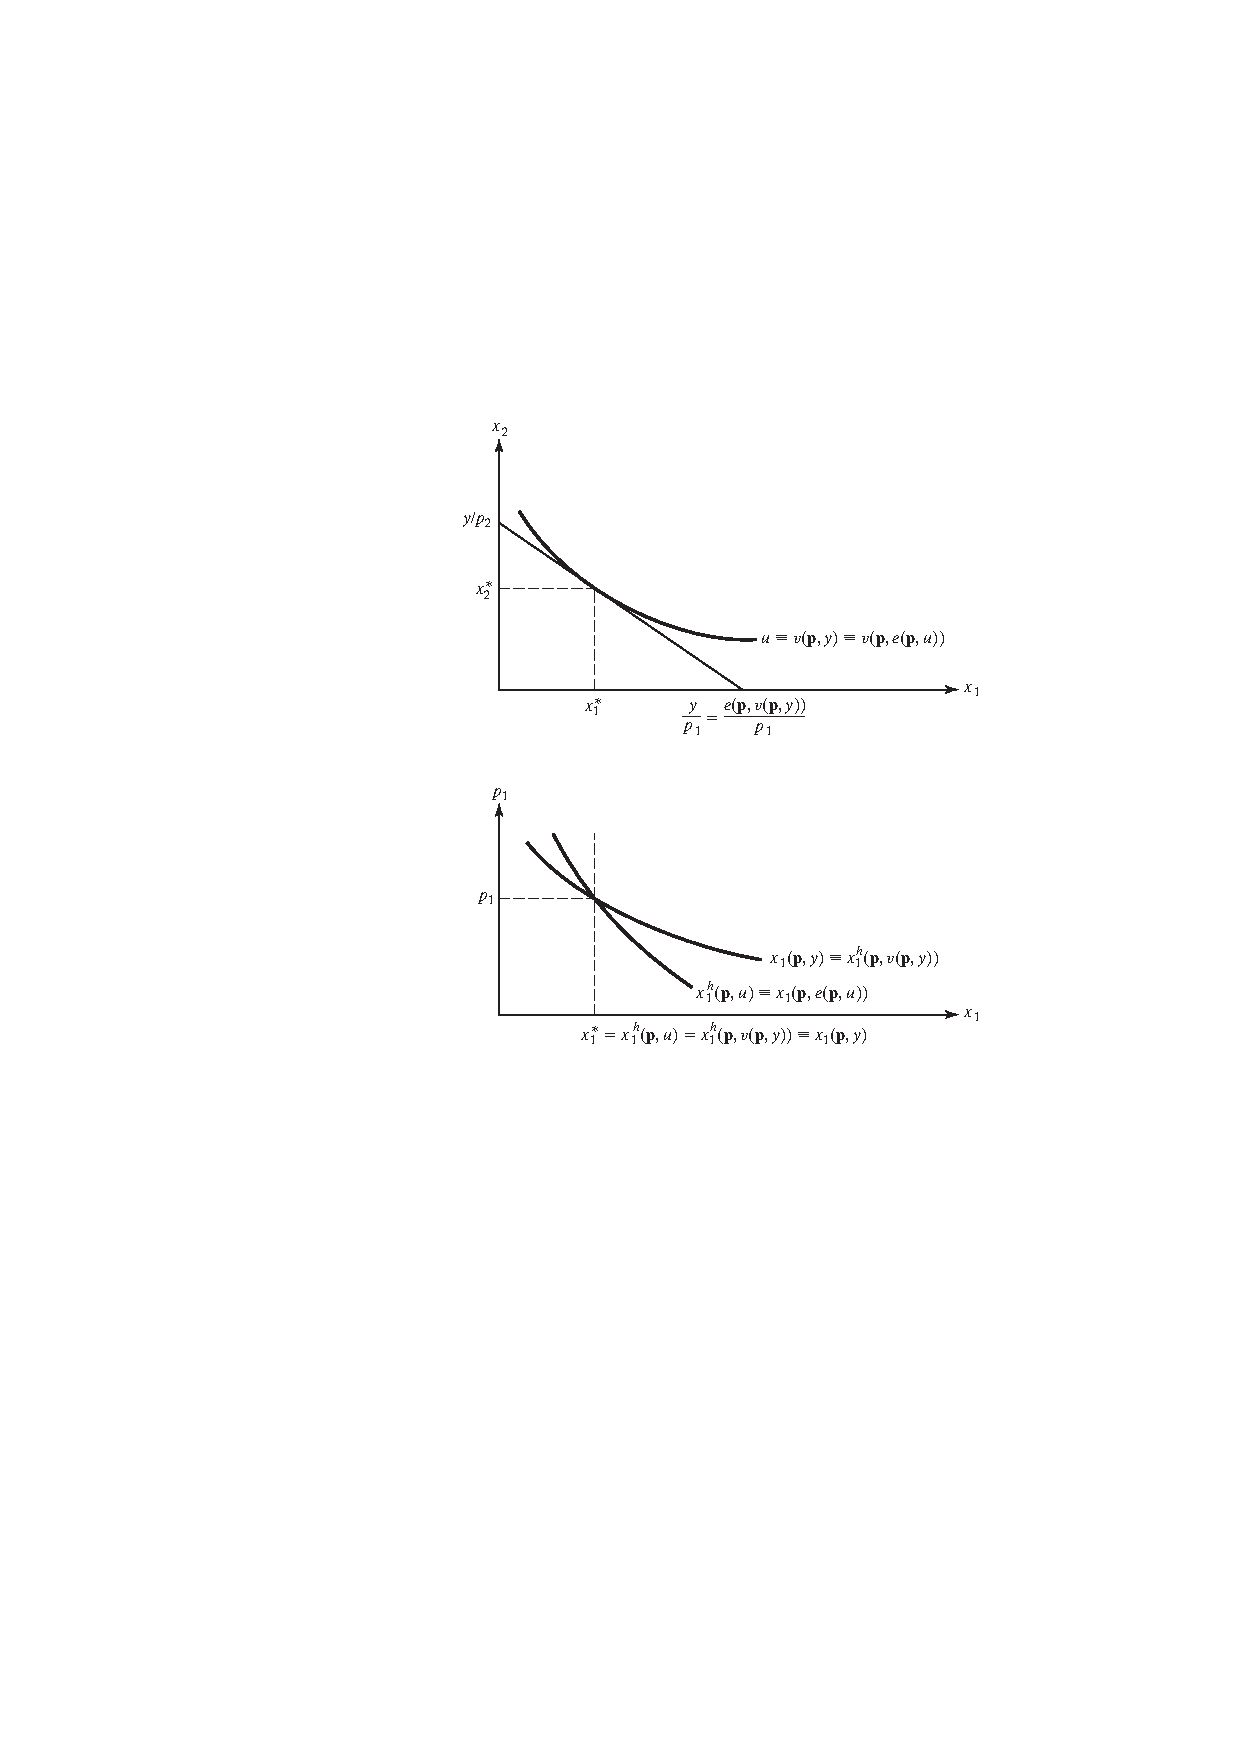
\includegraphics[width=10cm]{fig1-13.pdf}
  \caption{定理\ref{thm:thm1.3}和\ref{thm:thm1.4}的图示.}\label{fig1.13}
\end{figure}

图\ref{fig1.13}描述了定理\ref{thm:thm1.3}和\ref{thm:thm1.4}. 当价格为$\p$且收入为$y$时, 消费者通过选择最优消费束$x_1^\ast$和$x_2^\ast$达到了最大效用$u$, 可以将其视为给定的效用水平$v(\p,y)$, 点$(p_1,x^\ast_1)$将位于商品1的Marshall需求函数上.

接下来考虑消费者EMP, 假设寻找的是达到效用水平$u$的最小支出, 显然当价格为$\p$时, EMP的最低等支出线和UMP最大预算约束线重合, 而且EMP的选择也是$x_1^\ast$和$x_2^\ast$, 从而$(p_1,x_1^\ast)$位于商品1的Hicks需求曲线上.


\section{消费者的性质}
\subsection{收入效应与替代效应}
在消费者行为模型中, 一个重要的问题是当价格变动时需求数量如何变动. 一般地, 我们倾向于认为在其他条件不变时, 若某商品价格下降, 消费者会多买一些, 若价格上升, 她会少买一些, 然而图\ref{fig1.14}表明实际情况并非如此.

在图\ref{fig1.14}中, 总是假设消费者是追求效用最大化的, 她的偏好是严格单调和凸的, 且她面对的价格是市场决定的. 在第1张图中, 商品1价格下降导致其需求量上升; 在第2张图中, 商品1价格下降但其需求量不变; 在第3张图中, 商品1价格下降导致其需求量绝对减少.
\begin{figure}[htbp!]
  \centering
  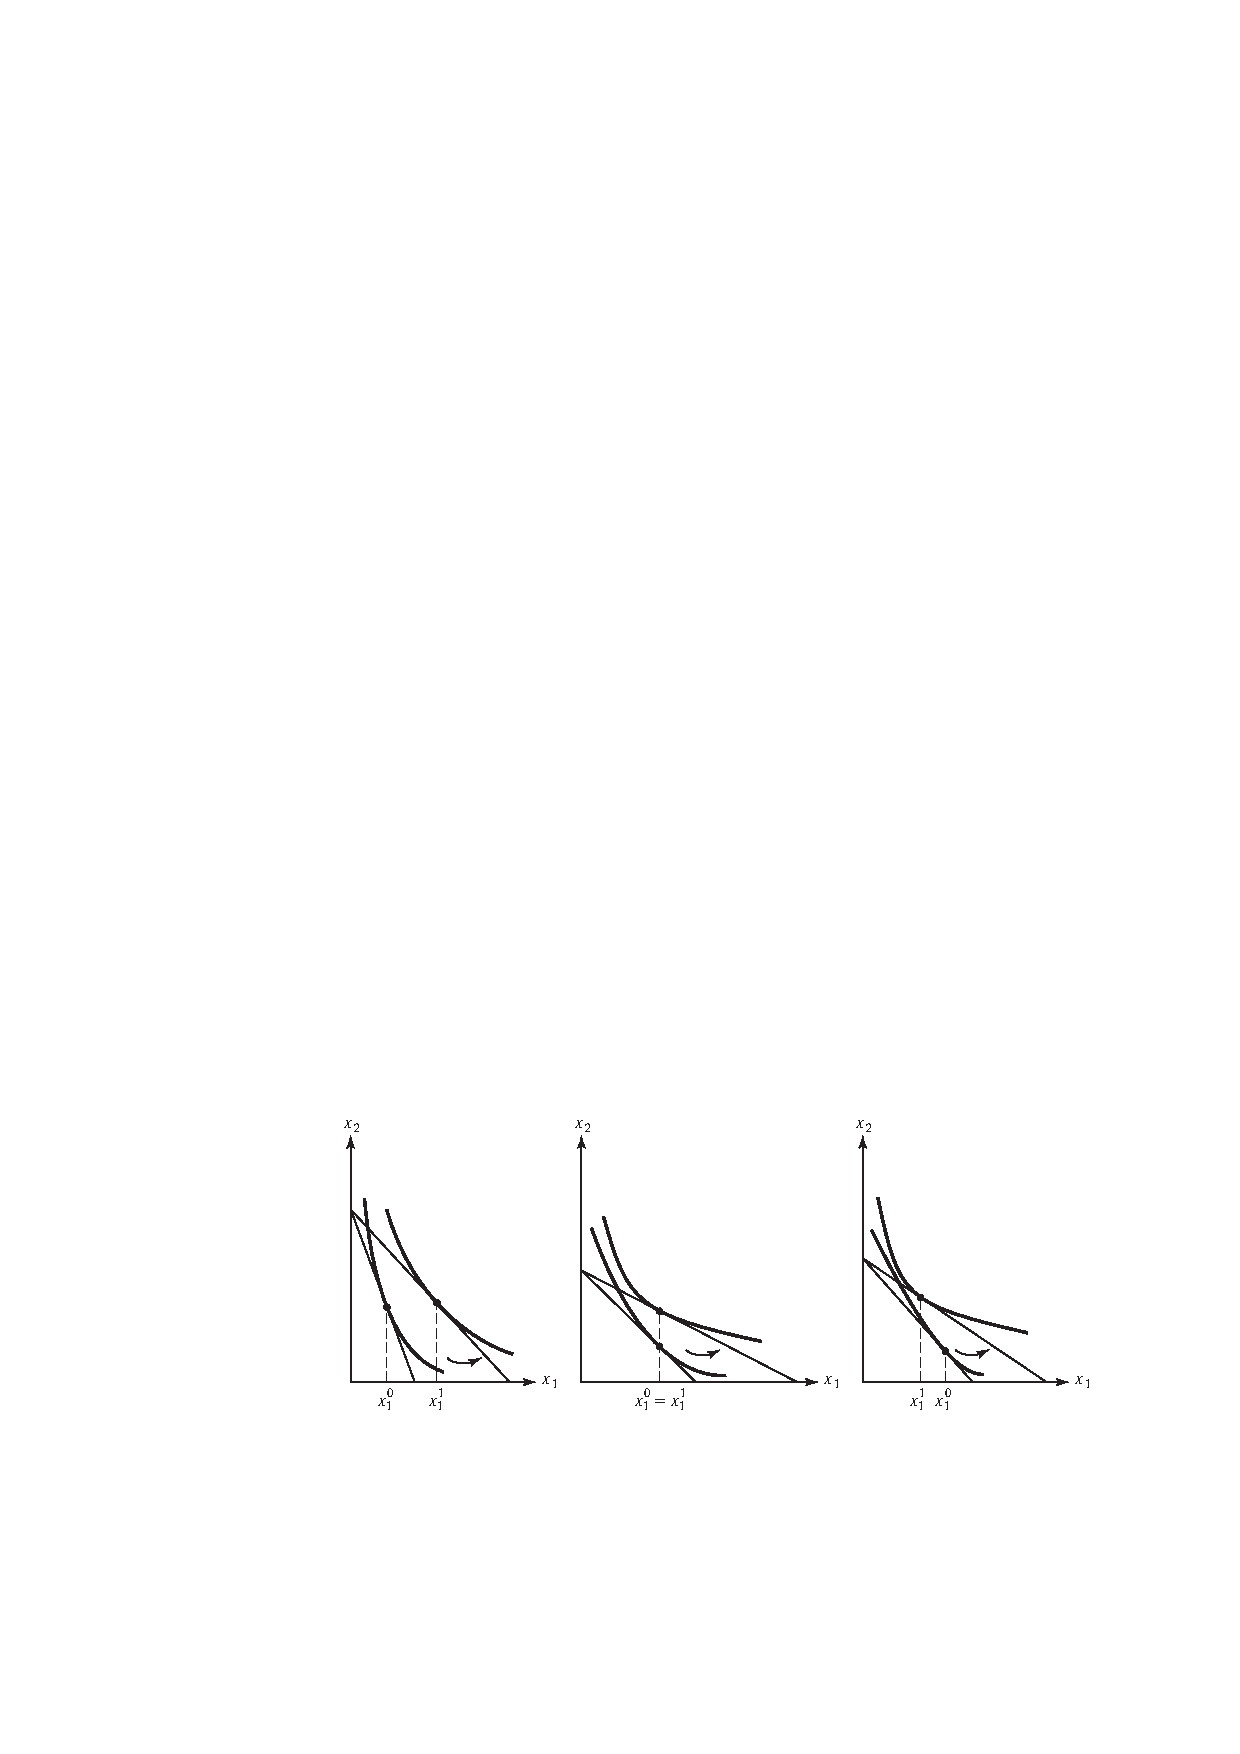
\includegraphics[width=15cm]{fig1-14.pdf}
  \caption{需求量对价格变动的反应.}\label{fig1.14}
\end{figure}

一方面, 商品1与其他商品相比该商品变得相对便宜了. 由于消费者想要所有各种商品, 即使消费者对所有商品的总购买力不变, 我们也可以预期他会用相对便宜的商品替代现在变得更昂贵的商品. 这种由于相对价格变动对需求量产生的效应称为\textbf{替代效应} (Substitution Effect, SE).

另一方面, 当某商品价格下降时, 消费者对所有商品的购买力实际上增加了, 这使得他会改变消费束中的某些或全部种类商品的数量, 只要他愿意. 这种由于购买力变动而对需求量产生的效应称为\textbf{收入效应} (Income Effect, IE).

价格变动的\textbf{总效应} (Total Effect, TE)为替代效应和收入效应之和, 这种分解可以遵循Hicks的方法来进行.

如图\ref{fig1.15}所示, 消费者最初面对的价格为$p_1^0$和$p_2^0$, 她的收入水平为$y$, 最初的购买量为$x_1^0$和$x_2^0$, 并且可以达到效用水平$u^0$. 现在假设商品1的价格从$p_1^0$下降到$p_1^1$而商品2的价格$p_2^0$维持不变, 价格变动的总效应体现为商品1的消费量增加至$x_1^1$而商品2的消费量下降至$x_2^1$.

现在对TE进行Hicks分解, 假想允许商品1的价格下降到$p_1^1$但维持效用水平$u^0$不变, 这种情形仿佛是允许消费者面对新的相对价格, 但却减少她的收入使得假想的预算约束线 (以虚线表示)与原本的平行, 此时消费者会增加商品1的消费量至$x_1^s$而将商品2的消费量减少至$x_2^s$, 这种价格变动就是商品1和商品2的Hicks替代效应. 现在只需解释消费量从$x_1^s$至$x_1^1$以及从$x_2^s$至$x_2^1$的变化, 这恰好是在新的价格水平和原有效用水平$u^0$时, 增加消费者的实际收入使得假想预算线平移至最终的预算线, 使得它与无差异曲线$u^1$相切, 这种价格变动称为商品1和商品2的Hicks收入效应, 描述的是纯粹由收入变动引起的需求量变动.

另一方面, 图\ref{fig1.15}显示了点$(p_1^0,x_1^0)$和$(p_1^1,x_1^1)$都在商品1的Marshall需求曲线上, 而点$(p_1^0,x_1^0)$和$(p_1^1,x_1^s)$都是商品1的Hicks需求曲线上. 换言之, Marshall需求曲线描述的是自价格 (own-price)变动引起的总效应, Hicks需求曲线描述的是自价格变动引起的纯Hicks替代效应, 两者差别可由Hicks收入效应解释.
\begin{figure}
  \centering
  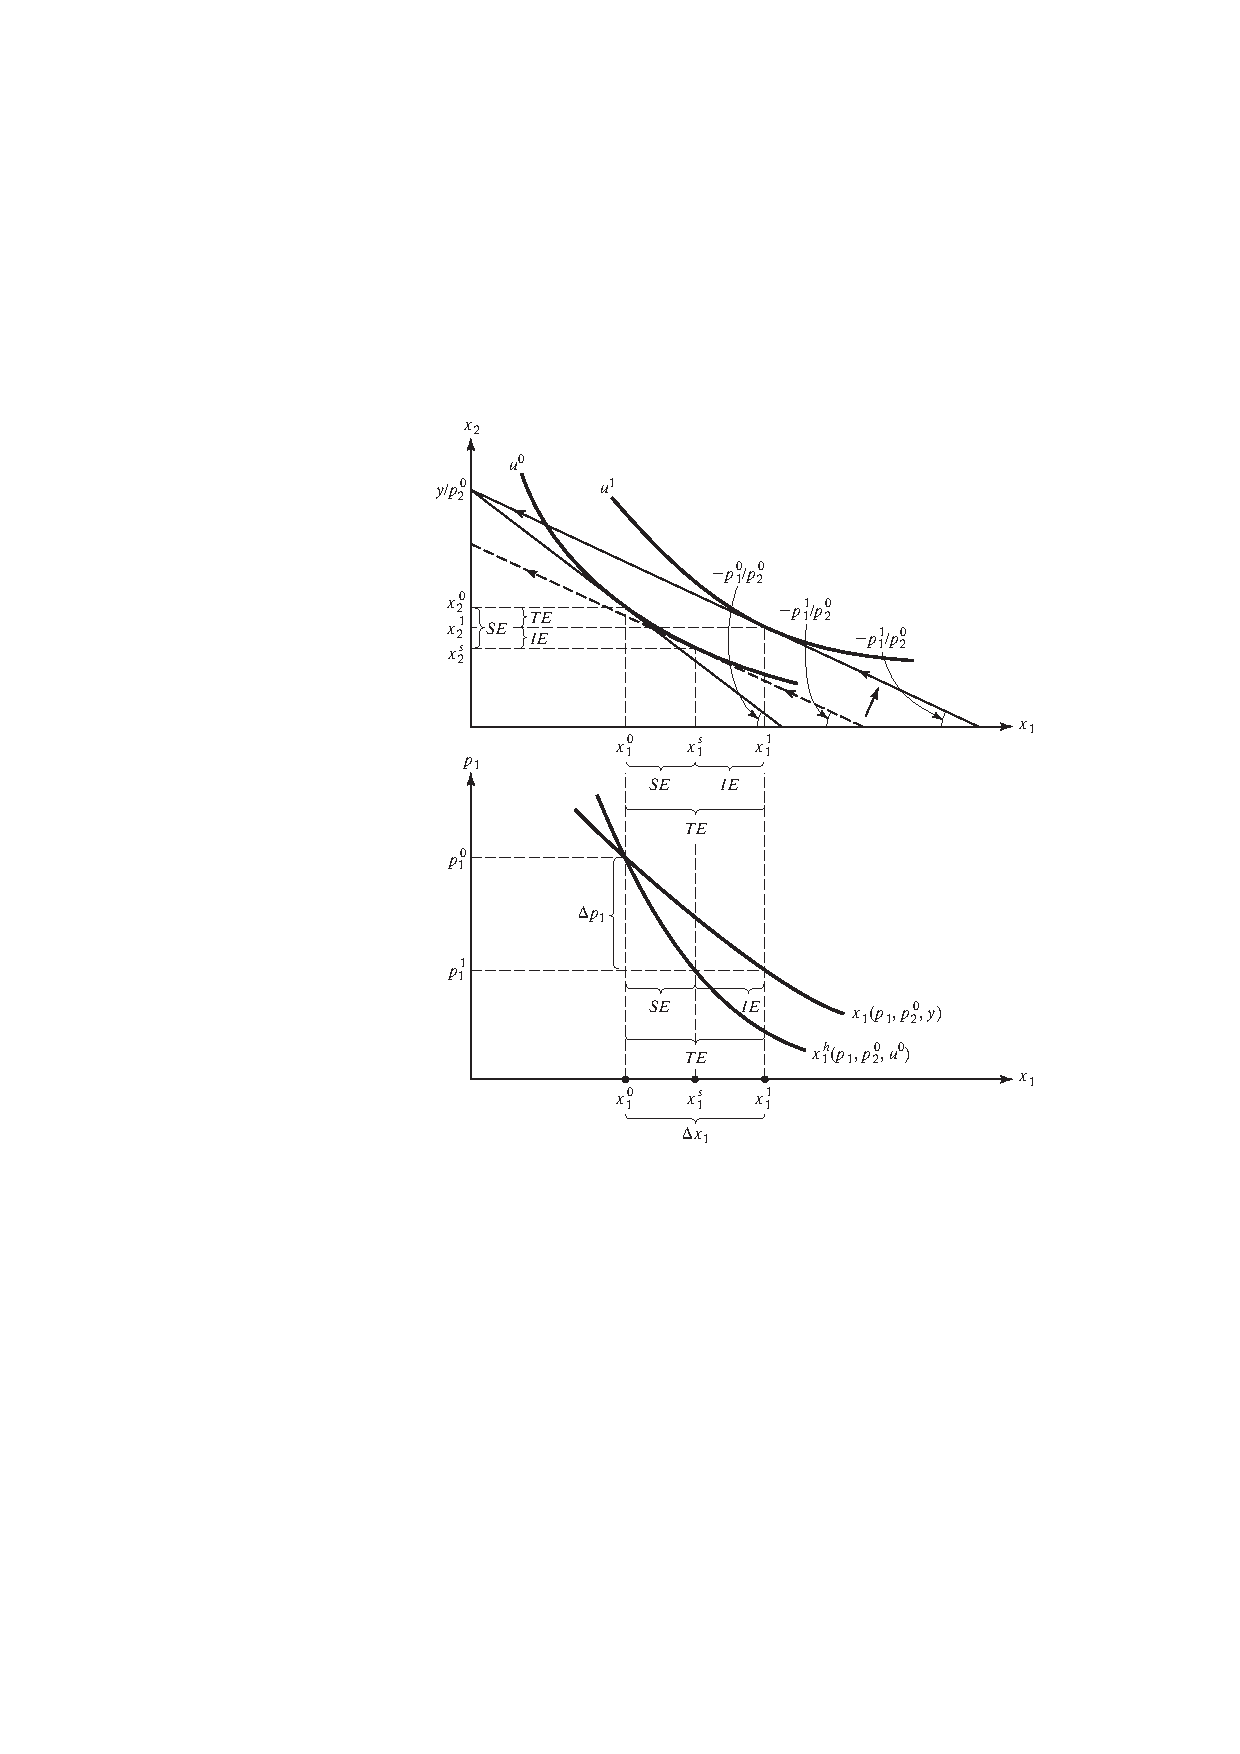
\includegraphics[width=10cm]{fig1-15.pdf}
  \caption{价格变动的Hicks分解.}\label{fig1.15}
\end{figure}

更一般地, 总效应、替代效应和收入效应可以用Slutsky方程表示, 它又称为“需求理论的基本方程”. 在接下来的部分, 总是规定假设\ref{pos:pos1.2}成立, 并且在需要时可以对函数微分.

\begin{theorem}[Slutsky方程]
  设$\x(\p,y)$表示消费者的Marshall需求方程组, 那么对于一切$(\p,y)\in\R_{++}^n\times\R_+$和$u=v(\p,y)$都有
  $$\frac{\partial x_i(\p,y)}{\partial p_j}=\frac{\partial x_i^h(\p,u)}{\partial p_j}-x_j(\p,y)\frac{\partial x_i(\p,y)}{\partial y},\quad i,j=1,\cdots,n$$
\end{theorem}
\begin{proof}
  根据定理\ref{thm:thm1.4}可知
  $$x_i^h(\p,u)=x_i(\p,e(\p,u))$$
  对于任意$\p\gg\mathbf{0}$和效用水平$u$成立, 上式两端同时对$p_j$微分得
  \begin{equation}\label{eq1.22}
    \frac{\partial x_i^h(\p,u)}{\partial p_j}=\frac{\partial x_i(\p,e(\p,u))}{\partial p_j}+\frac{\partial x_i(\p,e(\p,u))}{\partial y}\frac{\partial e(\p,u)}{\partial p_j}
  \end{equation}
  由于$u=v(\p,y)$是价格为$\p$收入为$y$时消费者所能实现的最大效用水平, 根据定理\ref{thm:thm1.3}可得
  \begin{equation}\label{eq1.23}
    e(\p,u)=e(\p,v(\p,y))=y
  \end{equation}
  根据Shephard引理可知
  $$\frac{\partial e(\p,u)}{\partial p_j}=x_j^h(\p,u)=x_j^h(\p,v(\p,y))$$
  再根据定理\ref{thm:thm1.4}可知
  \begin{equation}\label{eq1.24}
    \frac{\partial e(\p,u)}{\partial p_j}=x_j(\p,y)
  \end{equation}
  将式(\ref{eq1.23})和(\ref{eq1.24})代入到(\ref{eq1.22}), 稍加整理即可得到
  $$\frac{\partial x_i(\p,y)}{\partial p_j}=\frac{\partial x_i^h(\p,u)}{\partial p_j}-x_j(\p,y)\frac{\partial x_i(\p,y)}{\partial y}$$
  结论成立.
\end{proof}

Slutsky方程告诉我们总效应可以被分解为可观测到的收入效应和不可观测的替代效应, 根据该方程, 为了解释Marshall需求曲线的斜率 (需求量对自价格变动的反应), 必须知道Hicks需求曲线, 然而它是不可观测的, 但仍可以从消费者理论中获取它的信息.

\begin{theorem}
  设$x_i^h(\p,u)$是商品$i$的Hicks需求曲线, 那么$\partial x_i^h(\p,u)/\partial p_i\le0$.
\end{theorem}
\begin{proof}
  根据Shephard引理可知对任意$(\p,u)\in\R_{++}^n\times\mathcal{U}$都有
  $$\frac{\partial e(\p,u)}{\partial p_i}=x_i^h(\p,u)$$
  两边再对$p_i$求微分得
  $$\frac{\partial^2e(\p,u)}{\partial p_i^2}=\frac{\partial x_i^h(\p,u)}{\partial p_i},\quad i,j=1,\cdots,n$$
  由于$e$是关于$\p$的凹函数, 因此二阶偏导数非正, 由此证得命题.
\end{proof}
这一定理表明任何商品$i$的替代效应均非正, 因此当商品$i$的价格下降时, 替代效应必然非负, 但正如图\ref{fig1.14}所描述的那样, 商品价格下降时, 总效应也可能非正, 也即它的消费量也会下降, 称为Giffin悖论. 如果一种商品的需求量随着收入上升而增加, 则称它为\textbf{正常品} (normal good), 如果它的需求量随着收入上升而下降, 则称它为\textbf{劣等品} (inferior good).

\begin{corollary}
正常品的自价格下降会导致它的需求量上升; 如果商品自价格下降导致它的需求量减少, 那么该商品必定为劣等品.
\end{corollary}

为了了解更多关于替代效应的信息, 有必要继续探讨替代项的性质, 首先证明“交叉-替代项”是对称的.

\begin{proposition}\label{pro:pro1.3}
设$\x^h(\p,u)$表示消费者的Hicks需求方程组, 并且$e$是二阶连续可微的, 那么
$$\frac{\partial x_i^h(\p,u)}{\partial p_j}=\frac{\partial x_j^h(\p,u)}{\partial p_i},\quad i,j=1,\cdots,n$$
\end{proposition}
\begin{proof}
  根据Shephard引理可知
  $$\frac{\partial}{\partial p_j}\left[\frac{\partial e(\p,u)}{\partial p_i}\right]=\frac{\partial x_i^h(\p,u)}{\partial p_j}$$
  它等价于
  \begin{equation}\label{eq1.25}
    \frac{\partial^2e(\p,u)}{\partial p_j\partial p_i}=\frac{\partial x_i^h(\p,u)}{\partial p_j}
  \end{equation}
  对于一切$i,j=1,\cdots,n$成立, 根据Young定理可知, 支出函数的交叉二阶偏导的顺序是无所谓的, 也即
  $$\frac{\partial^2e(\p,u)}{\partial p_j\partial p_i}=\frac{\partial^2e(\p,u)}{\partial p_i\partial p_j}$$
  将该式与式(\ref{eq1.25})联立即可证得命题.
\end{proof}

\begin{proposition}\label{pro:pro1.4}
设$\x^h(\p,u)$表示消费者的Hicks需求, 并且
$$\sigma(\p,u)=\begin{pmatrix}
                 \frac{\partial x_1^h(\p,u)}{\partial p_1} & \cdots & \frac{\partial x_1^h(\p,u)}{\partial p_n} \\
                 \vdots &  & \vdots \\
                 \frac{\partial x_n^h(\p,u)}{\partial p_1} & \cdots & \frac{\partial x_n^h(\p,u)}{\partial p_n}
               \end{pmatrix}$$
为包含所有Hicks替代项的替代矩阵, 那么$\sigma(\p,u)$是半负定的.
\end{proposition}
\begin{proof}
  根据式(\ref{eq1.25})可得
  $$\begin{pmatrix}
                 \frac{\partial x_1^h(\p,u)}{\partial p_1} & \cdots & \frac{\partial x_1^h(\p,u)}{\partial p_n} \\
                 \vdots &  & \vdots \\
                 \frac{\partial x_n^h(\p,u)}{\partial p_1} & \cdots & \frac{\partial x_n^h(\p,u)}{\partial p_n}
               \end{pmatrix}=\begin{pmatrix}
                               \frac{\partial^2 e(\p,u)}{\partial p_1^2} & \cdots & \frac{\partial e(\p,u)}{\partial p_n\partial p_1} \\
                               \vdots &  & \vdots \\
                               \frac{\partial^2 e(\p,u)}{\partial p_1\partial p_n} & \cdots & \frac{\partial^2 e(\p,u)}{\partial p_n^2}
                             \end{pmatrix}$$
  上式右端的矩阵是支出函数$e$关于价格$\p$的Hessian矩阵, 由于$e$是$\p$的凹函数, 故而该矩阵为半负定的.
\end{proof}
\begin{theorem}\label{thm:thm1.5}
  设$\x(\p,y)$是消费者的Marshall需求方程组, 定义第$(i,j)$个Slutsky项为
  $$s_{ij}=\frac{x_i^h(\p,u)}{\partial p_j}+x_j(\p,y)\frac{\partial x_i(\p,y)}{\partial y}$$
  那么Slutsky矩阵$\mathbf{s}(\p,y)=(s_{ij})_{n\times n}$是对称和半负定的.
\end{theorem}
\begin{proof}
  设$u$是价格为$\p$收入为$y$时, 消费者效用可以达到的最大值, 于是$u=v(\p,y)$. 根据Slutsky方程可得第$(i,j)$个替代项为
  $$\frac{x_i^h(\p,u)}{\partial p_j}=\frac{x_i(\p,y)}{\partial p_j}+x_j(\p,y)\frac{\partial x_i(\p,y)}{\partial y}$$
  于是Slutsky矩阵$\mathbf{s}(\p,y)$的每一个元素恰好等于Hicks替代矩阵$\sigma(\p,u)$的相应元素. 根据命题\ref{pro:pro1.3}可知替代矩阵关于$u$是对称的, 而命题\ref{pro:pro1.4}又表明替代矩阵关于$u$是半负定的, 结论成立.
\end{proof}
定理\ref{thm:thm1.5}表明, 可以使用替代矩阵的知识推断出所有价格和收入变动对可观测的Marshall需求方程组的影响.


\subsection{弹性关系}
设$x_i(\p,y)$是消费者的Marshall需求函数, 预算平衡指的是对于每组价格和收入, 预算约束必然以等式形式成立, 也即
$$y=\sum_{i=1}^{n}p_ix_i(\p,y)$$
对一切$\p$和$y$成立, 因而如果任意单个商品价格或收入变动, 上式在变动前后仍成立. 因此, 消费者所有需求对价格和收入变动的反应需按照某种方式加总, 且这种方式要能保留变化发生后预算约束的等式仍然成立的这一性质, 为此需要介绍一些新的定义.

\begin{definition}
设$x_i(\p,y)$是消费者的Marshall需求函数, 那么
$$\eta_i=\frac{\partial x_i(\p,y)}{\partial y}\frac{y}{x_i(\p,y)}$$
称为商品$i$的收入弹性 (income elasticity), 并且
$$\epsilon_{ij}=\frac{\partial x_i(\p,y)}{\partial p_j}\frac{p_j}{x_i(\p,y)}$$
称为商品$i$的需求价格弹性 (demand price elasticity), 以及
$$s_i=\frac{p_ix_i(\p,y)}{y}$$
称为商品$i$的收入份额 (income share).
\end{definition}

$\eta_i$衡量的是消费者收入变动1\%导致商品$i$需求量变动的百分比. $\epsilon_{ij}$衡量的是价格$p_j$变动1\%引起的商品$i$需求量变动的百分比, 如果$j=i$, 则$\epsilon_{ij}$称为\textbf{自价格弹性} (own-price elasitcity), 如果$j\ne i$, 则$\epsilon_{ij}$称为关于$p_j$的\textbf{交叉价格弹性} (cross-price elasticity). $s_i$表示消费者花费在商品$i$上的金额占总收入的比例, 显然有$s_i\ge0$且$\sum_{i=1}^{n}s_i=y$.

通常而言, 如果$|\eta_i|>1$, 或者$|\epsilon_{ij}|>1$, 或者$|\epsilon_{ii}|>1$, 则称富有弹性; 如果是小于1, 则称为缺乏弹性; 如果是等于1, 则称为单位弹性. 对于富有弹性的商品, 则降低价格会增加销售额, 而对于缺乏弹性的商品, 降价则会导致销售额下降, 对于单位弹性的商品, 销售额不受价格变动的影响.
\begin{theorem}\label{thm:thm1.8}
  设$\x(\p,y)$是消费者的Marshall需求方程组, 那么以下关系成立
  \begin{enumerate}[label=\arabic*.]
    \item Engle加总: $\sum_{i=1}^{n}s_i\eta_i=1$;
    \item Cournot加总: $\sum_{i=1}^{n}s_i\epsilon_{ij}=-s_{ij}$, $j=1,\cdots,n$.
  \end{enumerate}
\end{theorem}
\begin{proof}
  1. 首先预算约束要求
  \begin{equation}\label{eq1.26}
    y=\p\cdot\x(\p,y)
  \end{equation}
  对一切价格$\p$和收入$y$成立, 上式两端对$y$求导得
  $$1=\sum_{i=1}^{n}p_i\frac{\partial x_i}{\partial y}$$
  上式右端同时乘以和除以$x_iy$得
  $$1=\sum_{i=1}^{n}\frac{p_ix_i}{y}\frac{\partial x_i}{\partial y}\frac{y}{x_i}$$
  也即$1=\sum_{i=1}^{n}s_i\eta_i$.

  2. 在式(\ref{eq1.26})两端对$p_j$求导得
  $$0=\left(\sum_{i\ne j}p_i\frac{\partial x_i}{\partial p_j}\right)+x_j+p_j\frac{\partial x_i}{\partial p_j}$$
  合并同类项并整理得到
  $$-x_j=\sum_{i=1}^{n}p_i\frac{\partial x_i}{\partial x_j}$$
  它等价于
  $$-\frac{p_jx_j}{y}=\sum_{i=1}^{n}\frac{p_ix_i}{y}\frac{\partial x_i}{\partial p_i}\frac{p_j}{x_i}$$
  也即$-s_j=\sum_{i=1}^{n}s_i\epsilon_{ij}$, $j=1,\cdots,n$.
\end{proof}
以上定理表明, 如果以收入份额为权重, 那么收入弹性的加权和为1 (Engle加总), 而需求价格弹性的加权和必定呈现出某种特别方式 (Cournot加总).


\chapter{消费者理论\rom{2}}
\section{对偶性}
\subsection{支出和消费者偏好}
考虑任何关于$\p$和$u$的函数$E(\p,u)$, 它可能是支出函数也可能不是, 假设它满足定理\ref{thm:thm1.6}中关于支出函数的全部性质, 也即它关于$u$是连续的、严格递增的、无上界的; 而且关于$\p$是递增的、 零次齐次的、凹的和可微的. 此时$E$看上去是个支出函数, 实际上它也必定是.

任意固定$(\p^0,u^0)\in\R_{++}^n\times\R_+$, 计算$E$在此处的函数值为$E(\p^0,u^0)$, 现在可以构造这个数在消费集中闭的\textbf{半空间} (half-space)
$$A(\p^0,u^0)=\{\x\in\R_+^n: \p^0\cdot\x\ge E(\p^0,u^0)\}$$
如图\ref{fig2.1}左侧所示, $A(\p^0,u^0)$是一个由包含于超平面$\p^0\cdot\x=E(\p^0,u^0)$上及其上方所有点构成的闭且凸的集合. 现在维持效用水平$u^0$不变, 改变价格水平$\p^1$, 可以构造闭的凸集
$$A(\p^1,u^0)=\{\x\in\R_+^n: \p^1\cdot\x\ge E(\p^1,u^0)\}$$
对所有$\p\gg\mathbf{0}$均这样构造, 可以得到无限个交集
\begin{equation}\label{eq2.1}
  A(u^0)=\bigcap_{\p\gg\mathbf{0}}A(\p,u^0)=\{\x\in\R_+^n: \p\cdot\x\ge E(\p,u^0),\forall\p\gg\mathbf{0}\}
\end{equation}
图\ref{fig2.1}右侧画出了有限个这样的交, 可以想象随着价格的增多, 阴影越接近某个拟凹实值函数的\textbf{优势集} (superior set).
\begin{figure}[htbp!]
  \centering
  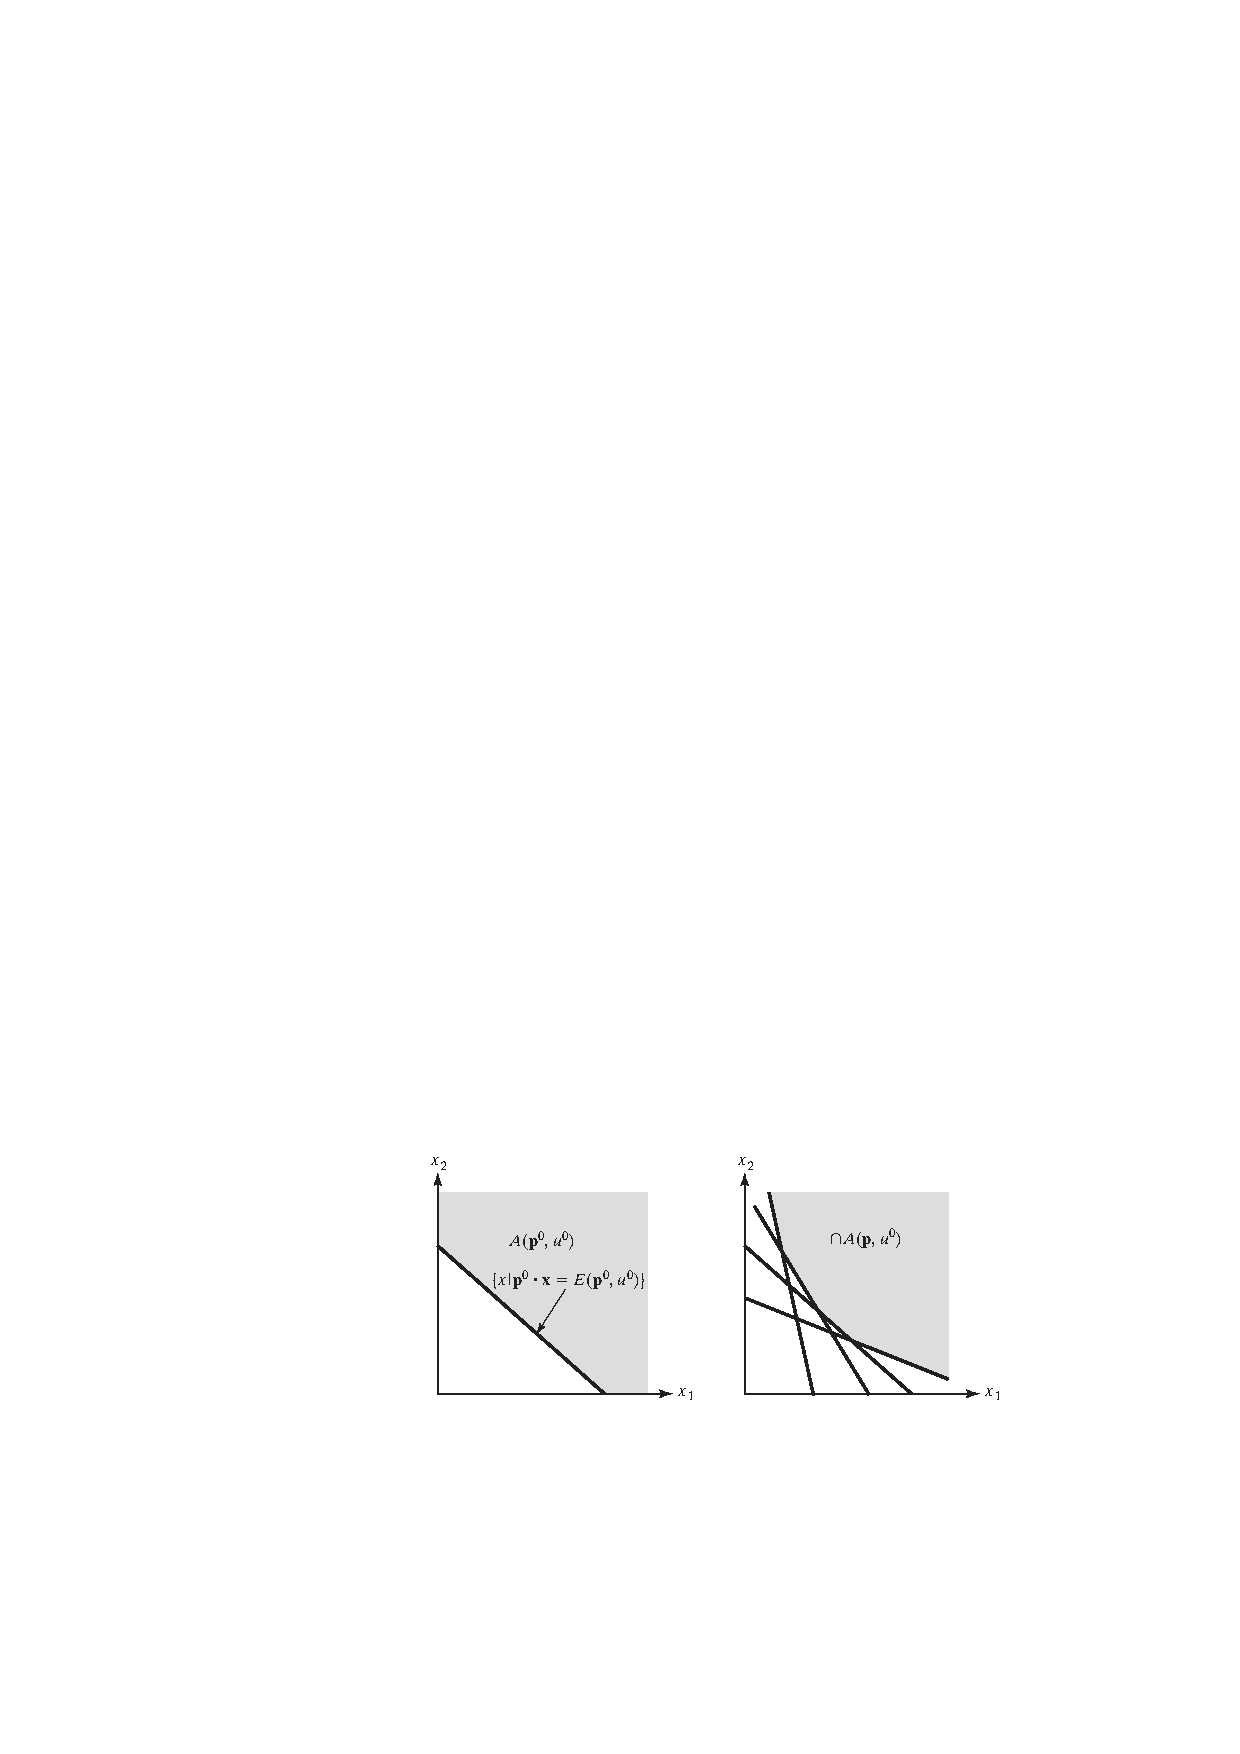
\includegraphics[width=15cm]{fig2-1.pdf}
  \caption{闭的半空间与有限个半空间的交集.}\label{fig2.1}
\end{figure}

\begin{theorem}\label{thm:thm2.1}
  如果$E:\R_{++}^n\times\R_+^n\to\R_+$满足定理\ref{thm:thm1.6}中的性质, 并且$A(u)$的定义与式(\ref{eq2.1})一致, 那么由下式给出的实值函数
  \begin{equation}\label{eq2.5}
    u(\x)=\max\{u\ge0: \x\in A(u)\}
  \end{equation}
  是单调递增的、无上界的和拟凹的.
\end{theorem}
\begin{proof}
  根据$A(u)$的定义, 可以将$u(\x)$改写为
  \begin{equation}\label{eq2.9}
    u(\x)=\max\{u\ge0: \p\cdot\x\geq E(\p,u),\forall \p\gg\mathbf{0}\}
  \end{equation}
  首先需要证明$u(\x)$是良好定义的, 也即需要证明集合
  $$B(\x)=\{u\ge0: \p\cdot\x\geq E(\p,u),\forall \p\gg\mathbf{0}\}$$
  包含着$u(\x)$的最大元素. 由于$E(\p,u)$关于$u$递增且无上界, 因此$B(\x)$有上界和上确界$\hat{u}$, 又因为$B(\x)$是闭的, 根据点集拓扑的知识可知$\hat{u}\in B(\x)$.\footnote{设$E$是一个非空且有上界的实数集, $\overbar{E}$是$E$的闭包, 令$y=\sup E$, 那么$y\in\overbar{E}$.}

  下面证明$u$是单调递增的. 考虑$\x^1\ge\x^2$, 于是对于任意$\p\gg\mathbf{0}$都有
  \begin{equation}\label{eq2.2}
    \p\cdot\x^1\ge\p\cdot\x^2
  \end{equation}
  根据$u$的定义可知
  \begin{equation}\label{eq2.3}
    \p\cdot\x^2\geq E(\p,u(\x^2))
  \end{equation}
  于是由式(\ref{eq2.2})和(\ref{eq2.3})可知
  $$\p\cdot\x^1\geq E(\p,u(\x^2))$$
  这就表明$\x^1\in A(u(\x^2))$, 因为$u(\x^1)$是使得$\x^1\in A(u)$的最大效用水平$u$, 所以$u(\x^1)\ge u(\x^2)$.

  这里略去$u$无上界的证明.

  最后证明$u$是拟凹函数, 也即对于任意$t\in[0,1]$, 都有
  $$u(t\x^1+(1-t)\x^2)\geq \min\{u(\x^1), u(\x^2)\}$$
  不妨令$u(\x^2)=\min\{u(\x^1), u(\x^2)\}$. 因为$u$是单调递增的, 故而$E(\p,u(\x^1))\geq E(\p,u(\x^2))$, 所以对任意$t\in[0,1]$都有
  \begin{equation}\label{eq2.4}
    tE(\p,u(\x^1))+(1-t)E(\p,u(\x^2))\geq E(\p,u(\x^2))
  \end{equation}
  根据$u$的定义, 对于任意$\p\gg\mathbf{0}$都有
  \begin{align*}
  \p\cdot\x^1&\geq E(\p,u(\x^1)) \\
  \p\cdot\x^2&\geq E(\p,u(\x^2))
  \end{align*}
  利用式(\ref{eq2.4})可得
  $$\p\cdot(t\x^1+(1-t)\x^2)\geq E(\p,u(\x^2))$$
  对一切$(\p,t)\in\R_{++}^n\times [0,1]$成立. 根据$u$的定义可知
  $$u(t\x^1+(1-t)\x^2)\geq u(\x^2)=\min\{u(\x^1),u(\x^2)\}$$
  这就得到了希望的结果.
\end{proof}

\begin{theorem}\label{thm:thm2.2}
  如果$E:\R_{++}^n\times\R_+\to\R_+$满足定理\ref{thm:thm1.6}中的性质, $u$是式(\ref{eq2.5})所定义的那样, 那么对于一切非负价格和效用都有
  $$E(\p,u)=\min_{\x\in\R_+^n}\p\cdot\x\quad\text{s.t.}\quad u(\x)\geq u$$
  也即$E(\p,u)$是由派生效用函数$u(\x)$生成的支出函数.
\end{theorem}
\begin{proof}
  任意固定$(\p,u)\in\R_{++}^n\times\R_+$, 假设$\x\in\R_+^n$满足$u(\x)\geq u^0$, 根据$u$的定义可知, 对于任意$\p\gg\mathbf{0}$都有
  $$\p\cdot\x\geq E(\p,u(\x))$$
  因为$E$是关于$u$的增函数, $u(\x)\geq u^0$, 故而
  $$\p\cdot\x\geq E(\p,u^0)$$
  也即对于任意给定的$\p^0\gg\mathbf{0}$, 我们已经得到对于任意$\x\in\R_+^n$都有
  $$E(\p^0,u^0)\leq \p^0\cdot\x\quad\text{s.t.}\quad u(\x)\ge u^0$$
  上式意味着
  $$E(\p^0,u^0)\leq\min_{\x\in\R_+^n}\p^0\cdot\x\quad\text{s.t.}\quad u(\x)\geq u^0$$
  现在需要证明上式是个等式, 实际上只需证明存在$\x^0\in\R_+^n$, 使得
  \begin{equation}\label{eq2.6}
    \p^0\cdot\x^0\leq E(\p^0,u^0),\quad u(\x^0)\geq u^0
  \end{equation}
  即可.

  由于$E$关于$\p$是可微和一次齐次的, 根据Euler定理可知对于任意$\p\gg\mathbf{0}$都有
  \begin{equation}\label{eq2.7}
    E(\p,u)=\frac{\partial E(\p,u)}{\partial\p}\cdot\p
  \end{equation}
  因为$E$是关于$\p$的凹函数, 故而
  \begin{equation}\label{eq2.8}
    E(\p,u^0)\leq E(\p^0,u^0)+\frac{\partial E(\p^0,u^0)}{\partial\p}\cdot(\p-\p^0)
  \end{equation}
  计算式(\ref{eq2.7})在$(\p^0,u^0)$处的值, 并将其与式(\ref{eq2.8})联立得到
  $$E(\p,u^0)\leq \frac{\partial E(\p^0,u^0)}{\partial\p}\cdot\p$$
  再令$\x^0=\partial E(\p^0,u^0)/\partial \p$, 现在可以将式(\ref{eq2.8})改写为
  $$\p\cdot\x^0\geq E(\p,u^0)$$
  根据$u$的定义可知$u(\x^0)$是使得$\p\cdot\x^0\geq E(\p,u)$的最大效用水平$u$, 因此必有$$u(\x^0)\geq u^0$$于是式(\ref{eq2.7})在$(\p^0,u^0)$处必有$E(\p^0,u^0)=\p^0\cdot\x^0$.
\end{proof}
上面两个定理告诉我们, 只要能写出一个关于价格和效用的函数, 而且这个函数满足定理\ref{thm:thm1.6}中的性质, 那么它将是某些偏好 (这些偏好满足常见的公理)的支出函数. 此外, 可以将这个函数关于产品价格微分, 从而得到相应的Hicks需求方程组. 如果消费者潜在的偏好是连续的且严格递增的, 我们可以逆转这个关于$u$的函数, 从而得到相应的间接效用函数, 应用Roy恒等式后可以推导出Marshall需求.
\subsection{凸性和单调性}
设$e$是效用函数$u$生成的支出函数, $u$的连续性足以保证$e$是定义良好的, 并且它还是连续函数. 进一步考虑函数$w:\R_+^n\to\R_+$, 它与式(\ref{eq2.9})是类似的, 也即
\begin{equation}\label{eq2.10}
  w(\x)=\max\{u\ge0:\p\cdot\x\ge e(\p,u),\forall\p\gg\mathbf{0}\}
\end{equation}
回顾定理\ref{thm:thm2.1}的证明过程, 无论$u$是否是单调递增和拟凹的, $w$都是单调递增和拟凹的.

\begin{figure}[htbp!]
  \centering
  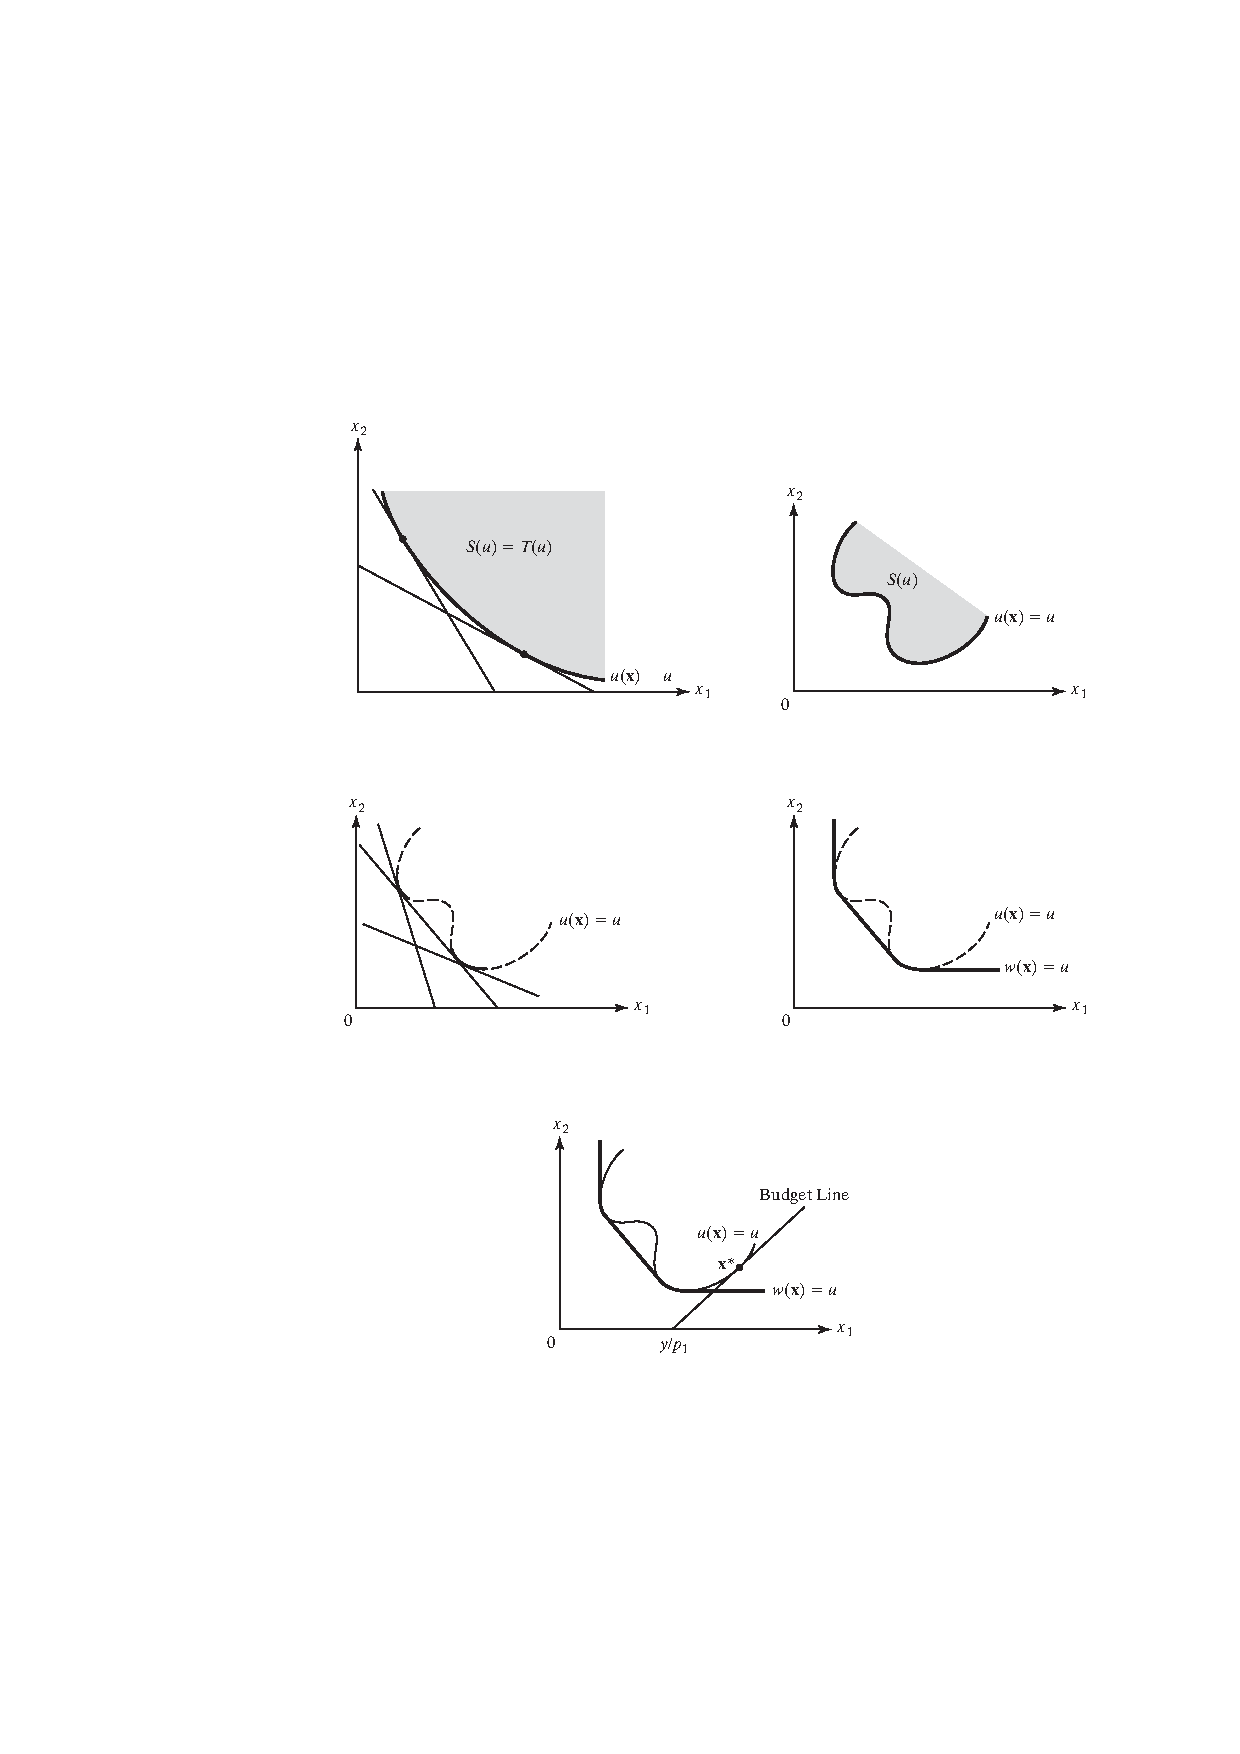
\includegraphics[width=12cm]{fig2-2.pdf}
  \caption{支出与效用的对偶性.}\label{fig2.2}
\end{figure}

对于任意的$u\ge0$, 设$u(\x)$是关于效用水平$u$的优势集为$S(u)$, 它包含于$w(\x)$关于效用水平$u$的优势集$T(u)$中, 由于$w(\x)$是拟凹函数, 因此$T(u)$是一个凸集.

如图\ref{fig2.2}的第一张所示, 若$u(\x)$碰巧是单调递增和拟凹的, 则$S(u)$的边界产生的无差异曲线$u(\x)=u$是凸的且斜率为负. 注意到$S(u)$边界上的每个点都是在价格向量$\p\gg\mathbf{0}$时实现效用$u$的最小支出消费束, 故而如果$u(\x^0)=u$, 那么存在某个$\p^0\gg\mathbf{0}$, 使得$e(\p^0,u)=\p^0\cdot\x^0$, 又因为$e$是关于$u$的递增函数, 这就意味着$w(\x^0)\leq u=u(\x^0)$. 另一方面, 根据$u$和$w$的定义可知$w(\x^0)\ge u(\x^0)$, 所以$w(\x^0)=u(\x^0)$总成立, 根据效用水平$u$的任意性, $w(\x)=u(\x)$对于一切$\x\in\R_+^n$成立.

图\ref{fig2.2}的剩余部分更有意思, 此时的$u(\x)$既非递增也非拟凹, $S(u)$产生了无差异曲线$u(\x)=u$, 但无差异曲线上的某些商品束在任何价格向量上都无法使实现效用水平$u$的支出最小化, 而的确可以使得支出最小化的商品束必有$u(\x)=w(\x)=u$, 由于$w(\x)$必定是严格递增和拟凹的, 因此$w(\x)=u$的曲线必定是粗实线的部分. 最终, $u(\x)$和$w(\x)$的区别仅仅在于$w(\x)$是单调递增和拟凹的.
\subsection{间接效用与消费者偏好}
假设$u(\x)$生成了间接效用函数$v(\p,y)$, 根据定义可知对于任意$\x\in\R_+^n$和$\p\gg\mathbf{0}$都有$v(\p,\p\cdot\x)\ge u(\x)$, 而且通常存在价格向量$\p^0$, 使得该不等式为等式, 也即
\begin{equation}\label{eq2.11}
  u(\x)=\min_{\p\in\R_{++}^n}v(\p,\p\cdot\x)
\end{equation}
因此式(\ref{eq2.11})表明即使我们仅知道某个效用函数$u(\x)$产生的间接效用函数, 我们也可以使用式(\ref{eq2.1})还原该效用函数.

\begin{theorem}
  设$u(\x)$在$\R_{++}^n$上是拟凹和可微的, 而且它的偏导数严格为正, 那么对于一切$\x\in\R_{++}^n$, $v(\p,\p\cdot\x)$在$\p\in\R_{++}^n$处达到最小值, 并且
  \begin{equation}\label{eq2.12}
    u(\x)=\min_{\p\in\R_{++}^n}v(\p,\p\cdot\x)
  \end{equation}
\end{theorem}
\begin{proof}
  根据之前的讨论, 式(\ref{eq2.12})的左端不会大于右端, 只要证明对于任意$\x\in\R_{++}^n$, 总存在$\p\gg\mathbf{0}$, 使得
  \begin{equation}\label{eq2.13}
    u(\x)=v(\p,\p\cdot\x)
  \end{equation}
  成立即可. 任意固定$\x^0\gg\mathbf{0}$, 令$\p^0=\nabla u(\x^0)$, 再令$\lambda^0=1$且$y^0=\p^0\cdot\x^0$, 于是
  \begin{align*}
  \frac{\partial u(\x^0)}{\partial x_i}-\lambda^0p_i^0&=0 \\
  \p^0\cdot\x^0&=y^0
  \end{align*}
  因此$(\x^0,\lambda^0)$是UMP
  $$\max_{\x\in\R_{++}^n}u(\x)\quad\text{s.t.}\quad\p^0\cdot\x^0=y^0$$
  的OFC, 又因为$u(\x)$在$\R_{++}^n$上是拟凹和可微的, 根据定理\ref{thm:thm1.7}可知, 这些条件足够保证$(\p,y)=(\p^0,y^0)$时$\x^0$是UMP的最优解. 由此可见$u(\x^0)=v(\p^0,y^0)=v(\p^0,\p^0\cdot\x^0)$, 根据$\x^0$的任意性可知结论成立.
\end{proof}

最后指出, 式(\ref{eq2.12})可以写成另一种更方便的形式. 由于$v(\p,y)$关于$(\p,y)$是零次齐次的, 于是对于$\p\cdot\x>0$必有$v(\p,\p\cdot\x)=v(\p/(\p\cdot\x),1)$, 此时式(\ref{eq2.12})可以改写为
\begin{equation}\label{eq2.14}
  u(\x)=\min_{\p\in\R_{++}^n}v(\p,1)\quad\text{s.t.}\quad\p\cdot\x=1
\end{equation}
\begin{theorem}[Hotelling-Wold对偶性]
  设直接效用函数$u$是可微的, 那么与收入水平$y=1$相伴的商品$i$的反需求函数为
  $$p_i(\x)=\frac{\partial u(\x)/\partial x_i}{\sum_{j=1}^{n}x_j[\partial u(\x)/\partial x_j]}\quad i=1,\cdots,n$$
\end{theorem}
\begin{proof}
  根据$\p(\x)$的定义, 对于所有$\x$都有$u(\x)=v(\p(\x),1)$和$\p(\x)\cdot\x=1$, 于是
  \begin{equation}\label{eq2.15}
    u(\x)=v(\p(\x),1)=\min_{\p\in\R_{++}^n}v(\p,1)\quad\text{s.t.}\quad\p\cdot\x=1
  \end{equation}
  定义Lagrange函数得到
  $$\mathcal{L}(\p,\lambda)=v(\p,1)-\lambda(\p\cdot\x-1)$$
  根据包络定理可得
  $$\frac{\partial u(\x)}{\partial x_i}=\frac{\partial\mathcal{L}(\x^\ast,\lambda^\ast)}{\partial x_i}=-\lambda^\ast p_i^\ast$$
  其中$\p^\ast=\p(\x)$, 并且$\lambda^\ast$是最优Lagrange乘子. 在上式两端同时乘以$x_i$并且在$i$上加总得到
  $$\sum_{i=1}^{n}x_i\frac{\partial u(\x)}{\partial x_i}=\lambda^\ast\sum_{i=1}^{n}p_i^\ast x_i=\lambda^\ast\sum_{i=1}^{n}p_i(\x)x_i=\lambda^\ast$$
  由于$\p(\x)\cdot\x=1$, 因此结论成立.
\end{proof}
\section{可积性问题}
在第1章, 我们已经证明追求效用最大化的消费者的Marshall需求函数必然满足零次齐次性、 预算平衡性、对称性、半负定性以及Engle加总和Cournot加总, 但是这里面有些条件是多余的. 事实上, 只有预算平衡性、对称性和半正定性才是真正独立的条件.

下面的定理表明, 预算平衡性与对称性意味着零次齐次性.
\begin{theorem}
  如果$\x(\p,y)$满足预算平衡性, 并且它的Slutsky矩阵$\mathbf{s}(\p,y)$是对称的, 那么它关于$\p$和$y$是零次齐次的.
\end{theorem}
\begin{proof}
  根据定理\ref{thm:thm1.8}的证明可知, 当预算平衡性成立时, 将预算约束对价格和收入进行微分
  \begin{align}
  \sum_{j=1}^{n}p_j\frac{\partial x_j(\p,y)}{\partial p_i}&=-x_i(\p,y) \label{eq2.16} \\
  \sum_{j=1}^{n}p_j\frac{\partial x_j(\p,y)}{\partial y}&=1 \label{eq2.17}
  \end{align}
  固定$(\p,y)$, 对任意$t>0$定义函数$f_i(t)=x_i(t\p,ty)$, 只需证明$f_i(t)$不随着$t$的变化而变化, 也即$f_i'(t)=0$对一切$t>0$成立.

  现在将$f_i$对$t$微分可得
  \begin{equation}\label{eq2.18}
    f_i'(t)=\sum_{j=1}^{n}\frac{\partial x_i(t\p,ty)}{\partial p_j}p_j+\frac{\partial x_i(t\p,ty)}{\partial y}
  \end{equation}
  根据预算平衡性可知$t\p\cdot\x(t\p,ty)=ty$, 将该式除以$t$可得
  \begin{equation}\label{eq2.19}
    y=\sum_{j=1}^{n}p_jx_j(t\p,ty)
  \end{equation}
  再用式(\ref{eq2.19})替代(\ref{eq2.18})得到
  $$f_i'(t)=\sum_{j=1}^{n}p_j\left[\frac{\partial x_i(t\p,ty)}{\partial p_j}+\frac{\partial x_i(t\p,ty)}{\partial y}x_j(t\p,ty)\right]$$
  上式方括号内的项是Slutsky矩阵$\mathbf{s}(\p,y)$的第$(i,j)$个元素, 根据假设可知该矩阵是对称的, 交换$i$和$j$的位置后可得
  \begin{align*}
  f_i'(t)&=\sum_{j=1}^{n}p_j\frac{\partial x_j(t\p,ty)}{\partial p_i}+x_i(t\p,ty)\sum_{j=1}^{n}p_j\frac{\partial x_j(t\p,ty)}{\partial p_i} \\
  &=\frac{1}{t}\sum_{j=1}^{n}tp_j\frac{\partial x_j(t\p,ty)}{\partial p_i}+x_i(t\p,ty)\frac{1}{t}\sum_{j=1}^{n}tp_j\frac{\partial x_j(t\p,ty)}{\partial p_i} \\
  &=\frac{1}{t}[-x_i(t\p,ty)]+x_i(t\p,ty)\frac{1}{t}\cdot1\\
  &=0
  \end{align*}
  其中倒数第二个等式是由式(\ref{eq2.16})和(\ref{eq2.17})在$(t\p,ty)$处的值得到的.
\end{proof}
现在, 如果$\x(\p,y)$是由UMP得到的Marshall需求方程组, 那么可以将观测到的消费者行为使用下列三个性质进行总结
\begin{itemize}
  \item 预算平衡性: $\p\cdot\x(\p,y)=y$;
  \item 半负定性: $\mathbf{s}(\p,y)$是半负定的;
  \item 对称性: $\mathbf{s}(\p,y)$是对称的.
\end{itemize}
可以证明, 以上三个性质是UMP推导出的可观测的消费者行为的全部性质, 除此之外, 追求效用最大化的消费者理论没有对需求行为施加其它独立的限制.

事实上, 如果某个关于价格和收入的向量值函数正好满足前面列举的三个条件, 那么的确存在生成这个需求函数的效用函数, 从消费者的效用还原出他的需求函数的问题称为\textbf{可积性问题} (integrability problem).

\begin{theorem}[可积性定理]
  连续可微函数$\x:\R_{++}^{n+1}\to \R_+^n$是某个严格递增的、严格拟凹的连续效用函数生成的需求函数, 当且仅当它满足预算平衡性、对称性和半负定性.
\end{theorem}
\begin{proof}
  由于已证得“仅当”的部分, 现在只证“当”这部分的论断, 也即证明如果某个函数$\x(\p,y)$满足预算平衡性、对称性和半负定性, 那么存在某个效用函数, 它可以生成$\x(\p,y)$作为它的需求函数.

  考虑任意一个支出函数$e(\p,u)$, 假设它由某个单调递增的拟凹效用函数$u(\x)$生成, 并且该效用函数生成的Marshall需求函数为$\x^m(\p,y)$. 首先证明, 如果$\x$和$e$的关系恰好如下所示
  \begin{equation}\label{eq2.20}
    \frac{\partial e(\p,u)}{\partial p_i}=x_i(\p,e(\p,u)),\quad \forall (\p,u)
  \end{equation}
  那么$\x(\p,y)$与效用函数$u(\x)$生成的$\x^m(\p,y)$相等.

  根据Shephard引理可知, 式(\ref{eq2.20})左侧等于$\x^h(\p,u)$, 式(\ref{eq2.20})意味着对任意的$(\p,u)$都有
  \begin{equation}\label{eq2.21}
    \x^h(\p,u)=\x(\p,e(\p,u))
  \end{equation}
  根据定理\ref{thm:thm1.4}可知
  \begin{equation}\label{eq2.22}
    \x^h(\p,u)=\x^m(\p,e(\p,u))
  \end{equation}
  联立式(\ref{eq2.21})和(\ref{eq2.22})得到
  $$\x(\p,e(\p,u))=\x^m(\p,e(\p,u))$$
  由于$e$作为支出函数, 对于每个固定的价格水平$\p$, 当$u$在其定义域内变动时, $e(\p,u)$取遍每个非负数, 故而对每个$(\p,y)$都有$\x(\p,y)=\x^m(\p,y)$.

  现在的任务简化为, 证明存在一个支出函数$e(\p,u)$, 使得它和$\x(\p,y)$的关系的确如式(\ref{eq2.20})所示. 假设偏微分方程组(\ref{eq2.20})的解为$e(\p,u)$, 在式(\ref{eq2.20})两端对$p_j$微分得到
  $$\frac{\partial^2 e(\p,u)}{\partial p_j\partial p_i}=\frac{\partial x_i(\p,e(\p,u))}{\partial p_j}+\frac{\partial e(\p,u)}{\partial p_j}\frac{\partial x_i(\p,e(\p,u))}{\partial y}$$
  令$y=e(\p,u)$, 根据Shephard引理和式(\ref{eq2.21})可将上式改写为
  \begin{equation}\label{eq2.23}
    \frac{\partial^2e(\p,u)}{\partial p_i\partial p_j}=\frac{\partial x_i(\p,y)}{\partial p_j}+x_j(\p,y)\frac{\partial x_i(\p,y)}{\partial y}
  \end{equation}
  根据Young定理可知, 式(\ref{eq2.23})左端关于$(i,j)$是对称的, 因此右端也是如此, 也即式(\ref{eq2.23})关于$(i,j)$的对称性是偏微分方程组(\ref{eq2.20})存在解的必要条件.

  事实上, 根据微分几何中的Frobenius定理, 这一对称条件也是(\ref{eq2.20})存在解的充分条件, 因此现在得到了解存在的充要条件. 注意到式(\ref{eq2.23})右端是与$\x(\p,y)$相关的Slutsky矩阵的第$(i,j)$项, 由于Slutsky矩阵关于$(i,j)$是对称的, 因此必定存在函数$e(\p,u)$满足式(\ref{eq2.20}).

  最后只需证明这样的函数$e(\p,u)$的确是支出函数, 通过验证$e(\p,u)$具有定理\ref{thm:thm1.6}中的性质, 根据定理\ref{thm:thm2.2}即可证得$e(\p,u)$是支出函数.
\end{proof}
如果我们想在有限的数据基础上估计消费者的需求函数, 而且还希望这个需求函数是由效用函数生成的, 有了可积性定理这个结论之后, 我们可以提出任何需求函数形式, 只要它满足预算平衡性、 对称性和负半定性即可. 而我们刚才已知道, 这样的需求函数必定是由效用函数产生的.
\section{显示偏好}
到目前为止, 我们处理需求理论的方法是假设消费者的偏好满足某些性质 (完备性、 传递性和严格单调性); 然后我们再推导出市场需求的所有可观测到的性质 (预算平衡性、 对称性以及Slutsky矩阵的半负定性).

Samuelson提出了另一种方法, 也即对消费者可观测的选择本身 (而非对不可观测到的偏好)做出若干简单和合理的假设, 然后在这些假设条件下进行推导. 这种方法的基本思想非常简明, 如果消费者选择消费束$\x^0$而非$\x^1$, 则称$\x^0$被显示偏好于$\x^1$.

\begin{definition}
对于任意两个组合$(\p^0,y^0)$和$(\p^1,y^1)$, 如果当$\x(\p^0,y^0)\neq \x(\p^1,y^1)$时有
$$\p^0\cdot\x(\p^1,y^1)\leq y^0\Rightarrow\p^1\cdot\x(\p^0,y^0)>y^1$$
那么称消费者的行为满足显示偏好弱公理 (Weak Axiom of Revealed Preference, WARP).
\end{definition}
换言之, 如果$\x(\p^0,y^0)$曾被显示偏好于$\x(\p^1,y^1)$, 那么$\x(\p^1,y^1)$绝不会被显示偏好于$\x(\p^0,y^0)$.

在图\ref{fig2.3}中, 消费者的行为都是在价格为$\p^0$时选择$\x^0$, 而在价格为$\p^1$时选择$\x^1$. 在左图中, 消费者的行为满足WARP, 因为她在本可以选择$\x^1$时的情形下选择了$\x^0$, 而当她选择$\x^1$时却买不起$\x^0$. 在右图中, 她在本可以选择$\x^1$的情形下选择了$\x^0$, 而她在选择$\x^1$时也可以选择$\x^0$但却没选, 因此这一消费行为违背WARP.

\begin{figure}[htbp!]
  \centering
  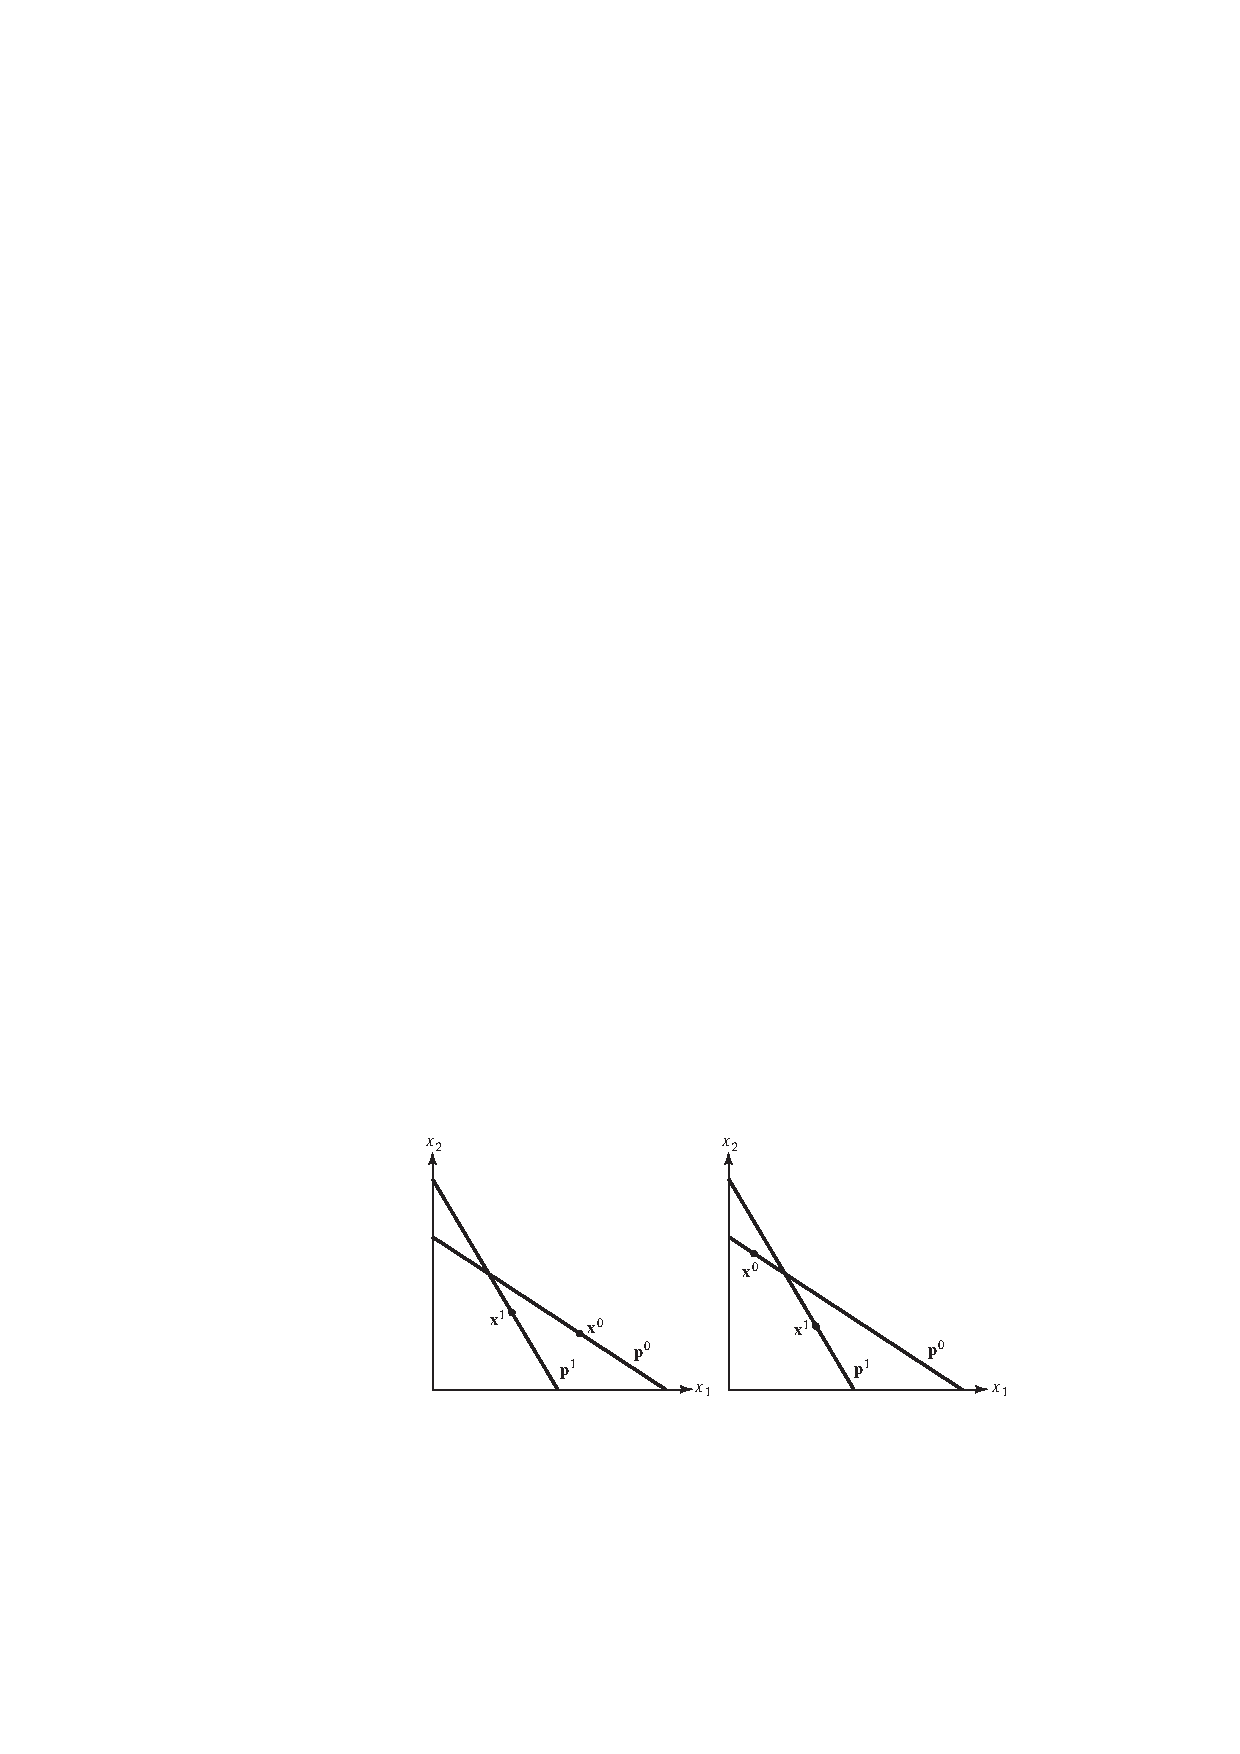
\includegraphics[width=12cm]{fig2-3.pdf}
  \caption{显示偏好弱公理.}\label{fig2.3}
\end{figure}

现在假设某消费者的行为满足WARP, 令$\x(\p,y)$表示在价格为$\p$且收入为$y$时该消费者的选择. 值得注意的是, 这个函数不是需求函数, 这是因为没有涉及到UMP, 所以$\x(\p,y)$只是表明了面临$(\p,y)$时消费者的选择, 此时称$\x(\p,y)$为\textbf{选择函数} (choice function). 除了WARP以外, 还对消费者的行为作出预算平衡性假设, 也即对于任意$\p\gg\mathbf{0}$, 选择函数$\x(\p,y)$满足预算平衡性$\p\cdot\x(\p,y)=y$.

实际上, 如果一个人的消费行为是理性的, 那么她的购买行为必然满足WARP, 也即WARP是理性偏好的必要条件. 然而, 满足WARP的消费行为却并不意味着理性消费, 除非该消费者购买的商品数量只有2种, 本节最后部分将会解释原因.

\begin{theorem}
如果WARP和预算平衡性成立, 那么选择函数$\x(\p,y)$关于$(\p,y)$是零次齐次的.
\end{theorem}
\begin{proof}
  假设价格为$\p^0$且收入为$y^0$时消费者的选择为$\x^0$, 再假设价格为$\p^1=t\p^0$且收入为$y^1=ty^0$时消费者的选择为$\x^1$, 其中$t>0$. 由此可知, 当消费者所有收入花完时, 必定有$\p^1\cdot\x^1=t\p^0\cdot\x^0$, 进而
  \begin{equation}\label{eq2.24}
    \p^0\cdot\x^1=\p^0\cdot\x^0
  \end{equation}
  以及
  \begin{equation}\label{eq2.25}
    \p^1\cdot\x^1=\p^1\cdot\x^0
  \end{equation}
  如果式(\ref{eq2.24})中的$\x^0$和$\x^1$是两个不同的消费束, 则WARP意味着式(\ref{eq2.25})左端必然严格小于右端, 这就产生矛盾, 因此$\x^0$和$\x^1$必定是相同的消费束.
\end{proof}

第1章已经提过, 商品价格变化对消费者的影响有两个方面, 其一是相对价格的变化, 其二是改变了消费者的实际收入. 为了研究WARP的意义, 需要隔离第一种效应.

当商品价格变动时, 相应调整消费者的收入水平, 使得他恰好能在新价格下买得起原来的消费束. 换言之, 如果消费者原来面对着价格$\p^0$和收入$y^0$时, 他选择消费束$\x(\p^0,y^0)$, 那么当价格变为$\p^1$时, 设想将消费者的收入调整为$y^1=\p^1\cdot\x(\p^0,y^0)$. 因此, 收入调整量为$\Delta y=\Delta \p\cdot\x(\p^0,y^0)$, 其中$\Delta \p=\p^1-\p^0$, 这种收入调整称为Slutsky补偿变化, 如图\ref{fig2.4}所示.

\begin{figure}[htbp!]
  \centering
  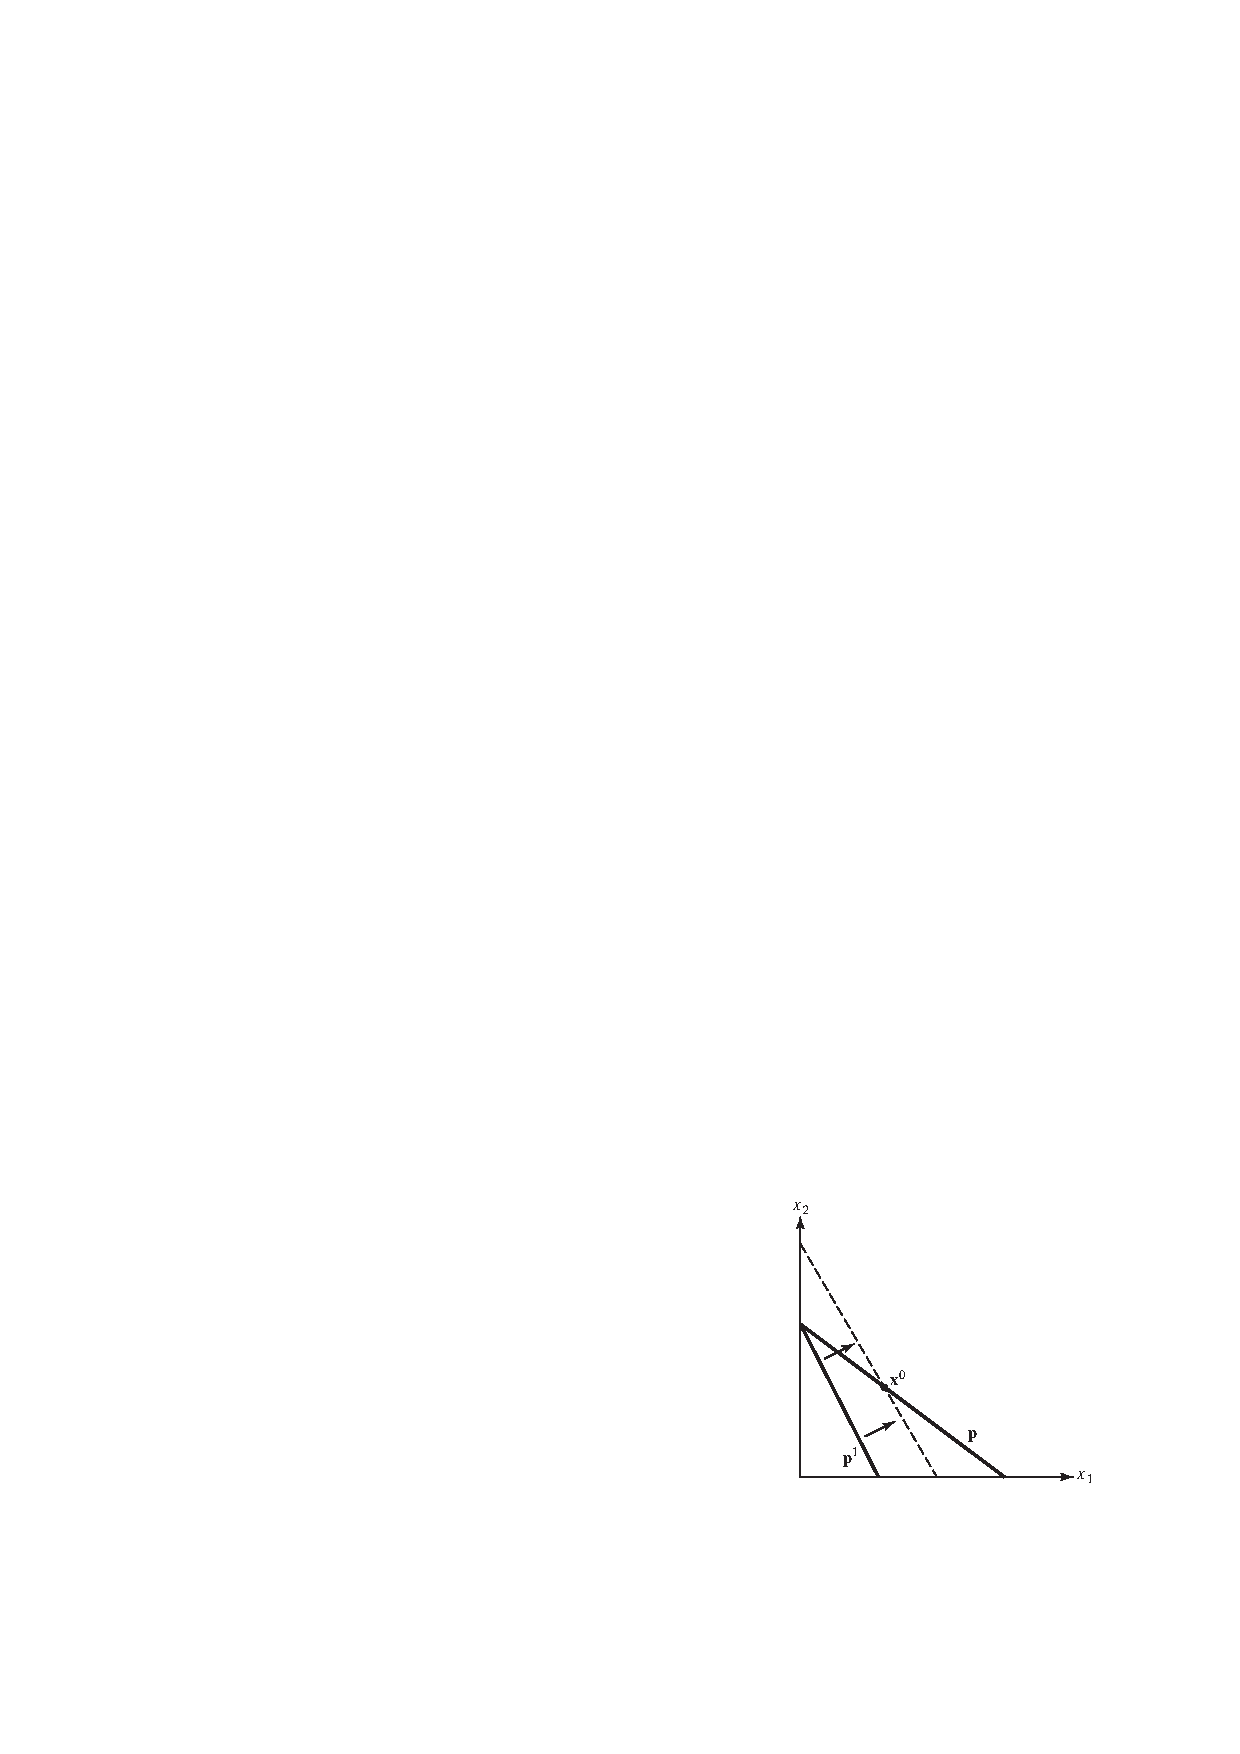
\includegraphics[width=7cm]{fig2-4.pdf}
  \caption{Slutsky补偿变化.}\label{fig2.4}
\end{figure}

\begin{theorem}\label{thm:thm2.3}
  如果WARP和预算平衡性成立, 那么$\x(\p,y)$满足WARP, 当且仅当对于从$(\p^0,y^0)$变化至$(\p^1,\p^1\cdot \x(\p^0,y^0))$的任何Slutsky补偿变化都有
  \begin{equation}\label{eq2.26}
    (\p^1-\p^0)\cdot[\x(\p^1,y^1)-\x(\p^0,y^0)]\le0
  \end{equation}
  且仅当$\x(\p^1,y^1)\neq \x(\p^0,y^0)$时, 严格不等式成立.
\end{theorem}
\begin{proof}
  先证明必要性: 显然当$\x(\p^1,y^1)=\x(\p^0,y^0)$时, 结果必然成立, 进而假设$\x(\p^1,y^1)\neq \x(\p^0,y^0)$, 式(\ref{eq2.26})左端可以写为
  \begin{equation}\label{eq2.27}
    \p^1\cdot[\x(\p^1,y^1)-\x(\p^0,y^0)]-\p^0\cdot[\x(\p^1,y^1)-\x(\p^0,y^0)]
  \end{equation}
  对于式(\ref{eq2.27})的第一项, 因为从$\p^0$至$\p^1$是Slutsky补偿变化, 故而$\p^1\cdot\x(\p^0,y^0)=y^1$, 根据预算平衡性可知$y^1=\p^1\cdot\x(\p^1,y^1)$, 因此
  \begin{equation}\label{eq2.28}
    \p^1\cdot[\x(\p^1,y^1)-\x(\p^0,y^0)]=0
  \end{equation}
  对于式(\ref{eq2.27})的第二项, 因为$\p^1\cdot\x(\p^0,y^0)=y^1$, 所以消费束$\x(\p^0,y^0)$是面对$(\p^1,y^1)$时消费者买得起的. 根据WARP可知$\p^0\cdot\x(\p^1,y^1)>y^0$, 再由预算平衡性得到
  \begin{equation}\label{eq2.29}
    \p^0\cdot[\x(\p^1,y^1)-\x(\p^0,y^0)]>0
  \end{equation}
  最后由式(\ref{eq2.27})、(\ref{eq2.28})和(\ref{eq2.29})就得到了想要的结果.

  再证明充分性: 首先证明对于任意$(\p^0,y^0)$和$(\p^1,y^1)$, 如果当$\p^0\cdot\x(\p^1,y^1)=y^0$和$\x(\p^1,y^1)\neq \x(\p^0,y^0)$时有$\p^1\cdot\x(\p^0,y^0)>y^1$, 那么WARP成立. 等价地, 只需证明这个论断的逆否命题: 如果WARP不成立, 则必然存在违反WARP的Slutsky补偿变化.

   假设存在违反WARP的情形: 考虑两个价格收入组合$(\p^0,y^0)$和$(\p^1,y^1)$, 使得$\x(\p^0,y^0)\neq \x(\p^1,y^1)$, 并且$\p^0\cdot\x(\p^1,y^1)\leq y^0$及$\p^1\cdot\x(\p^0,y^0)\leq y^1$. 若这两个不等式中任意一个以等式成立, 则它就是一个Slutsky补偿变化, 结论即刻证得, 因此下面均考虑严格不等式成立.

  现在任取$t\in(0,1)$, 使得
  $$\p\cdot\x(\p^0,y^0)\leq \p\cdot\x(\p^1,y^1)$$
  其中$\p=t\p^0+(1-t)\p^1$. 再令$y=\p\cdot\x(\p^0,y^0)$, 于是
  \begin{align*}
  ty^0+(1-t)y^1&>t\p^0\cdot\x(\p^0,y^0)+(1-t)\p^1\cdot\x(\p^0,y^0) \\
  &=y \\
  &=\p\cdot\x(\p,y) \\
  &=t\p^0\cdot\x(\p,y)+(1-t)\p^1\cdot\x(\p,y)
  \end{align*}
  因此要么$\p^0\cdot\x(\p,y)<y^0$, 要么$\p^1\cdot\x(\p,y)<y^1$, 或者二者兼具. 假设第一个不等号成立 (其余情形类似), 那么$\x(\p,y)\neq \x(\p^0,y^0)$, 并且$\p\cdot\x(\p^0,y^0)=y$和$\p^0\cdot\x(\p,y)<y^0$, 这就构造出了从$(\p^0,y^0)$到$(\p,y)$的违反WARP的Slutsky补偿变化.

  现在回到对充分性的证明. 假设式(\ref{eq2.26})成立并不意味着WARP, 此时必然存在从$(\p^0,y^0)$到$(\p,y)$的Slutsky补偿变化, 使得
  $$\x(\p,y)\neq \x(\p^0,y^0),\quad \p\cdot\x(\p^0,y^0)=y,\quad \p^1\cdot(\p,y)\leq y^1$$
  由于选择函数$\x(\p,y)$满足预算平衡性, 因此
  \begin{align*}
  \p\cdot[\x(\p^0,y^0)-\x(\p,y)]&=0 \\
  \p^0\cdot [\x(\p^0,y^0)-\x(\p,y)]&\ge0
  \end{align*}
  因此当$\x(\p^0,y^0)\neq \x(\p,y)$时必有
  $$(\p^1-\p)\cdot [\x(\p^1,y^1)-\x(\p,y)]\geq 0$$
  这就与式(\ref{eq2.26})产生矛盾, 因此WARP必然成立.
  \end{proof}
现在给定某个组合$(\p,y)$, 现在价格发生微分变化$\text{d}\p$, 现在对消费者进行Slutsky补偿$\text{d}y=\x(\p,y)\text{d}\p$, 定理\ref{thm:thm2.3}表明
\begin{equation}\label{eq2.30}
  \text{d}\p\cdot\text{d}\x\leq0
\end{equation}
根据链式法则可知
\begin{align*}
\text{d}\x&=\frac{\partial \x(\p,y)}{\partial\p}\text{d}\p+\frac{\partial \x(\p,y)}{\partial y}\text{d}y \\
&=\frac{\partial \x(\p,y)}{\partial\p}\text{d}\p+\frac{\partial \x(\p,y)}{\partial y}\x(\p,y)\text{d}\p
\end{align*}
由式(\ref{eq2.30})可知
$$\text{d}\p\cdot \mathbf{s}(\p,y)\cdot \text{d}\p\leq 0$$
其中$\mathbf{s}(\p,y)$为选择函数$\x(\p,y)$的Slutsky矩阵.

事实上, 我们已经证明了如果某个选择函数满足WARP和预算平衡性, 那么它的Slutsky矩阵是半负定的. 此时, 如果能证明某个选择函数的Slutsky矩阵是对称的, 那么根据可积性定理, 这个选择函数必定是Marshall需求函数. 另一方面, 容易证明如果$\x(\p,y)$碰巧是某个效用函数生成的Marshall需求函数, 那么$\x(\p,y)$必定满足WARP.

特别地, 当商品数量$n=2$时, WARP成立意味着Slutsky矩阵必定是对称的, 而当$n>2$时WARP无法保证Slutsky矩阵的对称性, 因此WARP和预算平衡性不等于效用最大化的假设. 值得注意的是, 如果将WARP加强为\textbf{显示偏好强公理} (Strong Axiom of Revealed Preference, SARP), 那么可以证明基于SARP之上的基于选择的需求理论, 在本质上等于基于偏好的需求理论.

\begin{definition}[显示偏好强公理]
Marshall需求函数$\x(\p,y)$满足SARP: 对于任意一列
$$(\p^1,y^1),(\p^2,y^2),\cdots,(\p^N,y^N)$$
如果对$n\le N-1$都有$\x(\p^{n+1},y^{n+1})\neq \x(\p^n,y^n)$, 并且$\p^n\cdot\x(\p^{n+1},y^{n+1})\leq y^n$对于一切$n\leq N-1$成立, 那么$\p^N\cdot\x(\p^1,y^1)>y^N$.
\end{definition}

显然, 当商品数量$n=2$时, WARP和SARP是等价的. 进一步, SARP排除了不可传递的显示偏好, 因此可用于诱导出一个完备且传递的偏好关系$\succsim$, 对于这个偏好关系存在着能使可观测到的行为理性化的效用函数. 无论是在SARP假设还是在效用最大化假设下, 消费者的需求都是齐次的, 而且Slutsky矩阵都是半负定的和对称的.

\section{不确定性下的选择}
\subsection{偏好}
之前我们假设消费者在他的消费集$X$中的所有消费束$\x$上拥有偏好关系. 在加入不确定性因素之后, 我们只要稍微变动一下视角即可. 我们将保留偏好关系的符号, 但我们不再假设消费者对消费束具有偏好关系, 而是对\textbf{彩票} (lottery)具有偏好关系. 更正式地说, 令$A=\{a_1,\cdots,a_n\}$表示结果 (outcome)的有限集, 这些$a_i$可以为消费束、金额数量或其它任何东西, 关键在于$a_i$本身涉及不确定性, 并且我们使用$A$作为彩票的基.

例如令$A=\{1,-1\}$, 其中$1$代表赢得1元钱的结果, $-1$代表输掉1元钱的结果, 彩票代表投掷一枚质地均匀的硬币, 如果正面朝上则赢1元, 反之则输1元, 这两种结果发生的概率均为$1/2$.

更一般地, \textbf{简单彩票} (simple lottery)对$A$中每个结果$a_i$赋予一个概率$p_i$, 显然每个$p_i$是非负的, 由于彩票必定导致$A$中某个结果发生, 因此$p_i$之和为1, 我们将简单彩票记为$(p_1\circ a_1,\cdots,p_n\circ a_n)$. 另外, 如果某个彩票的奖品也是彩票, 那么称这个彩票为\textbf{复合彩票} (compound lottery).

\begin{definition}[简单彩票]\label{def:def2.1}
令$A=\{a_1,\cdots,a_n\}$表示结果集, 那么$A$上的简单彩票空间为
$$\mathscr{L}_S\equiv\left\{(p_1\circ a_1,\cdots,p_n\circ a_n)\left|p_i\ge0, \sum_{i=1}^{n}p_i=1\right.\right\}$$
\end{definition}
特别地, 如果某些$p_i=0$, 那么就将相应的项从表达式中去掉. 如果对于每个$i$都有$p_i=1$, 那么将$1\circ a_i$简写为$a_i$, 表示必然发生结果$a_i$的彩票, 此时$\mathscr{L}_S$就包含了选择集$A$. 回到投掷硬币的例子中, 每个人都面对着简单彩票$(\frac{1}{2}\circ 1, \frac{1}{2}\circ -1)$.

不确定情形下的选择的就是彩票. 与消费者理论对应, 假设决策制定者在彩票集$\mathscr{L}$上有偏好$\succsim$, 接下来还需要对决策制定者的偏好关系$\succsim$设置一组公理, 称为\textbf{不确定性下的选择公理} (axiom of choice under uncertainty).

\begin{axiom}[完备性]\label{axi:axi2.1}
对于$\mathscr{L}$中的任意两个彩票$L$和$L'$, 要么$L\succsim L'$, 要么$L'\succsim L$.
\end{axiom}

\begin{axiom}[传递性]\label{axi:axi2.2}
对于$\mathscr{L}$中的任意三个彩票$L$, $L'$和$L''$, 如果$L\succsim L'$并且$L'\succsim L''$, 那么$L\succsim L''$.
\end{axiom}

由于可以将$A$中的每个$a_i$视作$\mathscr{L}$中的退化彩票, 公理\ref{axi:axi2.1}和\ref{axi:axi2.2}意味着$A$的有限个元素可以被$
\succsim$排序. 不失一般性, 假设我们已经对$A$的元素进行了标识, 从而$a_1\succsim a_2\succsim\cdots\succsim a_n$. 因此在所有彩票中, 最好的是以概率1产生结果$a_1$的彩票, 而最差的是以概率1产生结果$a_n$的彩票.

\begin{axiom}[连续性]\label{axi:axi2.3}
对于$\mathscr{L}$中的任意$L$, $L'$和$L''$, 集合$\{\alpha\in[0,1]:\alpha L+(1-\alpha)L'\succsim L''\}$和$\{\alpha\in[0,1]:L''\succsim \alpha L+(1-\alpha)L'\}$都是闭的.
\end{axiom}
举例来说, 假设$A=\{1000\text{元},\text{死亡}\}$, 对于绝大多数人都有$1000\text{元}\succ\text{死亡}$, 但得到1000元需要开车出门去拿, 而开车伴随着很小的死亡的正概率, 这样人就会在1000元和呆在家里中进行选择, 而连续性公理表明“出门取钱”和“死于车祸”的组合比“呆在家里”更受偏好.

事实上, 连续性公理排除了决策者对于某个发生概率为零的结果具有字典序偏好.

\begin{axiom}[独立性]\label{axi:axi2.4}
对于任意$L$, $L'$和$L''$以及$\alpha\in(0,1)$, 总有
$$L\succsim L'\Longleftrightarrow \alpha L+(1-\alpha)L''\succsim \alpha L'+(1-\alpha)L''$$
\end{axiom}
独立性公理是不确定性下的选择理论的核心, 它与之前基于偏好选择的理论不同, 正是因为不确定性结构的存在.

\begin{proposition}[复合彩票的简化]\label{pro:pro2.1}
对于任意彩票$L\in\mathscr{L}$, 如果$(p_1\circ a_1,\cdots,p_n\circ a_n)$是由$L$产生的简单彩票, 那么$(p_1\circ a_1,\cdots,p_n\circ a_n)\sim L$.
\end{proposition}
例如$A=\{a_1,a_2\}$, 某复合彩票以概率$\alpha$产生结果$a_1$, 以概率$1-\alpha$产生彩票, 该彩票以概率$\beta$产生结果$a_1$, 以概率$1-\beta$产生结果$a_2$, 那么决策者认为复合彩票和它产生的简单彩票$((\alpha+(1-\alpha)\beta)\circ a_1, (1-\alpha)(1-\beta)\circ a_2)$是无差异的.

\subsection{von Neumann-Morgenstern效用函数}
据我们对确定性条件下偏好的研究, 我们知道公理\ref{axi:axi2.1}和 \ref{axi:axi2.2}以及一些连续性假设应该足以保证存在着能代表$\succsim$的连续函数$u:\mathscr{L}\to\R$, 事实上, 不确定性选择公理的剩余部分则为这一函数提供了其它良好性质.
\begin{definition}
对于效用函数$u:\mathscr{L}\to\R$, 如果对于每一个$L\in\mathscr{L}$都有
$$u(L)=\sum_{i=1}^{n}p_iu(a_i)$$
其中$(p_1\circ a_1,\cdots,p_n\circ a_n)$是由$L$产生的简单彩票, 那么称$u$具有期望效用性质.
\end{definition}
我们说$u$具有\textbf{期望效用} (expected utility)性质, 等价于说$u$对每个彩票$L$指定了它可能产生的效用期望值, 其中$L$可能产生的每个效用伴随着该效用的实际概率, 并且$L$产生效用$u(a_i)$的实际概率正是$L$产生结果$a_i$的实际概率$p_i$.

我们称具有期望效应性质的效用函数为von Neumann-Morgenstern效用函数, 简记为vNM效用函数, 根据不确定性选择公理\ref{axi:axi2.1}-\ref{axi:axi2.4}, 可以证明vNM效用函数的存在性.

\begin{theorem}[期望效用定理]
  设$\mathscr{L}$上的偏好关系$\succsim$满足公理\ref{axi:axi2.1}-\ref{axi:axi2.4}, 那么在$\mathscr{L}$上存在能代表$\succsim$的vNM效用函数$u:\mathscr{L}\to\R$.
\end{theorem}
\begin{proof}
  本质上需要证明对于任意$L, L'\in\mathscr{L}$, 总有
  $$L\succsim L'\Longleftrightarrow\sum_{i=1}^{n}u_ip_i\geq \sum_{i=1}^{n}u_ip_i'$$
  为简单起见, 假设$\mathscr{L}$中存在最好的彩票$\overbar{L}$和最差的彩票$\ubar{L}$, 也即对于任意$L\in\mathscr{L}$都有$\overbar{L}\succsim L\succsim \ubar{L}$. 如果$\overbar{L}\sim\ubar{L}$, 那么$\mathscr{L}$中的所有彩票都是无差异的, 结论自然成立, 现在只需假设$\overbar{L}\succ\ubar{L}$, 按以下6个步骤证明.

  Step 1: 如果$L\succ L'$且$\alpha\in(0,1)$, 那么$g\succ \alpha L+(1-\alpha)L'\succ L'$.

  根据独立性公理可以直接得到
  $$L=\alpha L+(1-\alpha)L\succ \alpha L+(1-\alpha)L'\succ \alpha L'+(1-\alpha)L'=L'$$
  这表明决策者对两个彩票非退化组合的偏好位置必定严格位于她对这两个彩票偏好之间.

  Step 2: 对于$\alpha,\beta\in(0,1)$, 总有$\beta\overbar{L}+(1-\beta)\ubar{L}\succ \alpha\overbar{L}+(1-\alpha)\ubar{L}$当且仅当$\beta>\alpha$.

  假设$\beta>\alpha$, 注意到
  $$\beta\overbar{L}+(1-\beta)\ubar{g}=\gamma\overbar{L}+(1-\gamma)[\alpha\overbar{L}+(1-\alpha)\ubar{L}]$$
  其中$\displaystyle\gamma=\frac{\beta-\alpha}{1-\alpha}\in[0,1]$. 根据Step 1可知$\overbar{L}\succ \alpha\overbar{L}+(1-\alpha)\ubar{L}$, 再次利用Step 1可知
  $$\gamma\overbar{L}+(1-\gamma)[\alpha\overbar{L}+(1-\alpha)\ubar{L}]\succ \alpha\overbar{L}+(1-\alpha)\ubar{L}$$
  这就证明了$\beta\overbar{L}+(1-\beta)\ubar{L}\succ \alpha\overbar{L}+(1-\alpha)\ubar{L}$.

  反过来假设$\beta\leq\alpha$, 如果$\beta=\alpha$, 那么有$\beta\overbar{L}+(1-\beta)\ubar{L}\sim \alpha\overbar{L}+(1-\alpha)\ubar{L}$, 故而只需假设$\beta<\alpha$. 根据刚才的结论, 只需调换$\alpha$和$\beta$的位置即可得到$\alpha\overbar{L}+(1-\alpha)\ubar{L}\succ\beta\overbar{L}+(1-\beta)\ubar{L}$.

  Step 3: 对于任意$L\in\mathscr{L}$, 存在唯一的$\alpha_L$使得$[\alpha_L\overbar{L}+(1-\alpha_L)\ubar{L}]\sim L$.

  定义集合$\{\alpha\in[0,1]: \alpha\overbar{L}+(1-\alpha)\ubar{L}\succsim L\}$和$\{\alpha\in[0,1]: L\succsim \alpha\overbar{L}+(1-\alpha)\ubar{L}\}$, 根据$\succsim$的完备性和连续性可知它们都是闭集, 而且$\alpha\in[0,1]$至少位于这两个集合中的一个. 由于这两个集合非空且$[0,1]$是连通的, 因此存在某个$\alpha_L$使得$\alpha_L\overbar{L}+(1-\alpha_L)\ubar{L}\sim L$, 根据Step 2的结论可以得到$\alpha_L$的唯一性.

  Step 4: 如果函数$u:\mathscr{L}\to\R$对每一个$L\in\mathscr{L}$都能赋于$u(L)=\alpha_L$, 那么$u$可以代表偏好关系$\succsim$.

  根据Step 3可知, 对于任意$L, L'\in\mathscr{L}$总有
  $$L\succsim L'\Longleftrightarrow \alpha_L\overbar{L}+(1-\alpha_L)\ubar{L}\succsim \alpha_{L'}\overbar{L}+(1-\alpha_{L'})\ubar{L}$$
  因此根据Step 2有$L\succsim L'$当且仅当$\alpha_L\geq \alpha_{L'}$, 也即$u(L)\geq u(L')$.

  Step 5: 效用函数$u:\mathscr{L}\to\R$具有期望效用性质当且仅当它是线性的, 也即对于任意$k$个彩票, $(\alpha_1,\cdots,\alpha_k)\ge 0$和$\sum_{j=1}^k \alpha_j=1$, 总有
  \begin{equation}\label{eq2.31}
    u\left(\sum_{j=1}^{k}\alpha_j L_j\right)=\sum_{j=1}^{k}\alpha_ju(L_j)
  \end{equation}

  假设$u:\mathscr{L}\to\R$满足式(\ref{eq2.31}), 可以将彩票$L=(p_1\circ a_1,\cdots, p_n\circ a_n)$作为退化彩票$(a_1,\cdots,a_n)$的凸组合, 也即$L=\sum_{i} p_ia_i$, 这里$i=1,\cdots,n$, 于是$u(L)=u(\sum_ip_ia_i)=\sum_ip_iu(a_i)$, 因此$u:\mathscr{L}\to\R$具有期望效用性质.

  假设$u:\mathscr{L}\to\R$具有期望效用性质, 对于任意复合彩票$(\alpha_1\circ L_1,\cdots,\alpha_k\circ L_k)$, 其中$L_j=(p_1^j\circ a_1,\cdots, p_n^j\circ a_n)$, 该复合彩票的退化彩票为$L'=\sum_j\alpha_jL_j$, 其中$j=1,\cdots,k$. 根据期望效用性质可知式(\ref{eq2.31})成立.

  Step 6: 对于任意$L\in\mathscr{L}$, 每个指定$u(L)=\alpha_L$的效用函数$u:\mathscr{L}\to\R$是线性的.

  根据Step 5可知, 只需证明对于任意$L$, $L'\in\mathscr{L}$和$\beta\in[0,1]$, 总有
  $$u[\beta L+(1-\beta)L']=\beta u(L)+(1-\beta)u(L')$$
  即可. 根据定义可知
  $$L\sim u(L)\overbar{L}+[1-u(L)]\ubar{L}$$
  以及
  $$L'\sim u(L')\overbar{L}+[1-u(L')]\ubar{L}$$
  再由独立性公理可得
  \begin{align*}
  \beta L+(1-\beta)L'&\sim\beta\{u(L)\overbar{L}+[1-u(L)]\ubar{L}\}+(1-\beta)L' \\
  &\sim\beta\{u(L)\overbar{L}+[1-u(L)]\ubar{L}\}+(1-\beta)\{u(L')\overbar{L}+[1-u(L')]\ubar{L}\}
  \end{align*}
  也即在代数上等价于
  $$\beta L+(1-\beta)L'\sim [\beta u(L)+(1-\beta)u(L')]\overbar{L}+[1-\beta u(L)-(1-\beta)u(L')]\ubar{L}$$
  根据Step 4中对效用函数$u$的构造可得
  $$u[\beta L+(1-\beta)L']=\beta u(L)+(1-\beta)u(L')$$
  证明完毕.
\end{proof}

\begin{example}\label{exp:exp2.1}
假定$A=\{10\text{元},4\text{元},-2\text{元}\}$, 分别记为$a_1$, $a_2$和$a_3$. 这里的最好结果是获得10元, 最差结果是损失2元, 并且这两个结构的概率未知, 但概率之和为1. 现在问消费者, 当获得10元的概率为多少时, 他才会认为我们构造的最好-最差彩票组合与以概率1得到$a_i$是无差异的?

假定消费者回答
\begin{align*}
10\text{元}&\sim (1\circ 10\text{元}, 0\circ -2\text{元}) \\
4\text{元}&\sim (0.6\circ 10\text{元}, 0.4\circ -2\text{元}) \\
-2\text{元}&\sim (0\circ 10\text{元}, 1\circ -2\text{元})
\end{align*}
那么可以定义$u(10\text{元})=1$, $u(4\text{元})=0.6$, $u(-2\text{元})=0$, 最好结果的效用为1, 最差结果的效用为0, 而中间结果的效用取决于消费者对风险的态度. 可以看到, 消费者将以概率1获得4元, 与不确定条件获得5.2元的期望收入视作一样好, 说明他有规避风险的态度.

以上信息已经足够我们对这些结果涉及的彩票进行排序, 考虑
\begin{align*}
L_1&=(0.2\circ 4\text{元}, 0.8\circ 10\text{元}) \\
L_2&=(0.07\circ -2\text{元}, 0.03\circ 4\text{元}, 0.9\circ 10\text{元})
\end{align*}
如果消费者对彩票的偏好满足公理\ref{axi:axi2.1}-\ref{axi:axi2.4}, 根据vNM效用函数的性质可得
\begin{align*}
u(L_1)&=0.2u(4\text{元})+0.8u(10\text{元})=0.920 \\
u(L_2)&=0.07u(-2\text{元})+0.03u(4\text{元})+0.9u(10\text{元})=0.918
\end{align*}
此时消费者对彩票$L_1$的期望效用大于$L_2$, 因此他必定偏好于$L_1$. 值得注意的是, 尽管期望收入$E(L_1)=8.8\text{元}<E(L_2)=8.98\text{元}$, 但消费者仍然偏好于$L_1$, 这是因为彩票$L_2$面临损失的风险过高.
\end{example}

\begin{example}[$\,$Allais悖论]
假设有三种货币商品, 一等奖赢500万, 二等奖赢100万, 三等奖什么也没有, 将它们分别记作$a_1$, $a_2$和$a_3$. 假设彩票
\begin{align*}
L_1&=(0\circ a_1, 1\circ a_2, 0\circ a_3) \\
L_1'&=(0.10\circ a_1,0.89\circ a_2, 0.01\circ a_3) \\
L_2&=(0\circ a_1, 0.11\circ a_2, 0.89\circ a_3) \\
L_2'&=(0\circ a_1, 0.10\circ a_2, 0.90\circ a_3)
\end{align*}
某人需要在$L_1$和$L_1'$之间, 以及$L_2$和$L_2'$之间进行选择.

根据期望效用理论, 倘若某人认为$L_1\succ L_1'$, 则可以用vNM效用函数表示为
$$u(a_1)>0.10u(a_1)+0.89u(a_2)+0.01u(a_3)$$
在两侧同时加上$0.89u(a_3)-0.89u(a_2)$得到
$$0.11u(a_2)+0.89u(a_3)>0.10u(a_1)+0.90u(a_3)$$
也即他必定认为$L_2\succ L_2'$.

然而, 根据实际的调查结果, 绝大多数人认为$L_1\succ L_1'$且$L_2'\succ L_2$, 这就和期望效用理论矛盾. 究其原因, 主要是在于独立性公理不成立, 期望效用理论不适用.

\end{example}

\begin{example}
在确定性条件下的消费者理论中, 效用值本身只有序数含义, 也即效用函数的严格单调变化可以表示的偏好关系$\succsim$是相同的, 然而与代表消费者对彩票偏好的vNM效用函数来说, 效用值具有基数含义.

为了看到这一点, 假设$A=\{a,b,c\}$且$a\succ b \succ c$, 那么由偏好关系$\succsim$的完备性和连续性可知存在$p\in (0,1)$使得
$$b\sim (p\circ a, (1-p\circ c)$$
令$u$是能代表$\succsim$的vNM效用函数, 那么
$$u(b)=u[p\circ a, (1-p)\circ c]=pu(a)+(1-p)u(c)$$
从而
$$\frac{u(a)-u(b)}{u(b)-u(c)}=\frac{1-\alpha}{\alpha}$$
也即对于具有期望效用形式的效用函数来说, 效用之差是有含义的.

显然, 对于任何vNM效用函数, 它的严格递增变换很有可能不再是个vNM效用函数 (它仍是一个效用函数, 但是不具有期望效用性质). 下面的定理表明, 如果我们想让它的单调变换也具有期望效用性质, 那么我们只能进行正仿射变换.
\end{example}
\begin{theorem}
  假设$u:\mathscr{L}\to\R$是代表$\mathscr{L}$上的偏好关系$\succsim$的vNM效用函数, 那么$\tilde{u}$是$\mathscr{L}$上关于$\succsim$的另一个vNM效用函数, 当且仅当存在$\beta>0$和$\gamma\in\R$, 使得对于任意$L\in\mathscr{L}$都有$\tilde{u}(L)=\beta u(L)+\gamma$.
\end{theorem}
\begin{proof}
  在简单彩票空间$\mathscr{L}$中选取$\overbar{L}$和$\ubar{L}$, 使得对于任意$L\in\mathscr{L}$都有$\overbar{L}\succ L\succ \ubar{L}$.

  设$(p_1\circ a_1,\cdots,p_n\circ a_n)$是由$L\in\mathscr{L}$产生的简单彩票, $L$可以视为退化彩票$(a_1,\cdots,a_n)$的凸组合, 也即$L=\sum_i p_ia_i$, 再设$u$是$\mathscr{L}$上关于$\succsim$的vNM效用函数, 于是
  \begin{align*}
  \tilde{u}(L)&=\beta u(L)+\gamma=\beta\left[\sum_{i=1}^{n}p_iu(a_i)\right]+\gamma \\
  &=\sum_{i=1}^{n}p_i[\beta u(a_i)+\gamma]=\sum_{i=1}^{n}p_i\tilde{u}(a_i)
  \end{align*}
  根据上一定理中的Step 5可知效用函数$\tilde{u}$具有期望效用性质, 因此是vNM效用函数.

  反过来, 需要证明如果$\tilde{u}$和$u$具有相同的期望效用形式, 那么存在$\beta>0$和$\gamma\in\R$, 使得对于一切$L\in\mathscr{L}$都有$\tilde{u}(L)=\beta u(L)+\gamma$.

  任取$L\in\mathscr{L}$, 将$\lambda_L\in[0,1]$定义为
  $$u(L)=\lambda_Lu(\overbar{L})+(1-\lambda_L)u(\ubar{L})$$
  故而
  \begin{equation}\label{eq2.32}
    \lambda_L=\frac{u(L)-u(\ubar{L})}{u(\overbar{L})-u(\ubar{L})}
  \end{equation}
  由于$u$是vNM效用函数, 故而$\lambda_Lu(\overbar{L})+(1-\lambda_L)u(\ubar{L})=u[\lambda_L\overbar{L}+(1-\lambda_L)\ubar{L}]$, 又因为$u$可以代表偏好关系$\succsim$, 因此$L\sim \lambda_L\overbar{L}+(1-\lambda_L)\ubar{L}$. 这样的话, 由于$\tilde{u}$也是vNM效用函数且代表相同的偏好, 那么
  \begin{align*}
  \tilde{U}(L)&=\tilde{u}[\lambda_L\overbar{L}+(1-\lambda_L)\ubar{L}] \\
  &=\lambda_L\tilde{u}(\overbar{L})+(1-\lambda_L)\tilde{u}(\ubar{L}) \\
  &=\lambda_L[\tilde{u}(\overbar{L})-\tilde{u}(\ubar{L})]+\tilde{u}(\ubar{L})
  \end{align*}
  将式(\ref{eq2.32})代入后得$\tilde{u}(L)=\beta u(L)+\gamma$, 其中
  $$\beta=\frac{\tilde{u}(\overbar{L})-\tilde{u}(\ubar{L})}{u(\overbar{L})-u(\ubar{L})},\quad \gamma=\tilde{u}(\ubar{L})-u(\ubar{L})\frac{\tilde{u}(\overbar{L})-\tilde{u}(\ubar{L})}{u(\overbar{L})-u(\ubar{L})}$$

\end{proof}

\subsection{决策者的风险态度}
在示例\ref{exp:exp2.1}中, 我们构造的vNM效用函数反映了消费者具有规避风险的愿望, 现在可以将其正式地定义为\textbf{风险厌恶} (risk aversion).

考虑结果集$A=\R_+$, 尽管结果集包含不可数个结果, 但我们假定只对有限多个结果指定严格为正的概率, 此时的简单彩票形式为$(p_1\circ w_1,\cdots,p_n\circ w_n)$, 这里的$n$为某个正整数, $w$代表非负财富水平, 非负概率$p_1,\cdots,p_n$之和为1. 最后, 假设vNM效用函数是可微的, 并且$u'(w)>0$.

\begin{remark}
事实上, 由于财富水平是连续变量, 我们可以将彩票空间$\mathscr{L}$视为非负财富量$w$的所有分布函数$F(w)$构成的集合, 将她的理性偏好$\succsim$定义在$\mathscr{L}$上, 并使用Lebesgue积分来定义vNM效用函数, 这是更一般化的表达.
\end{remark}

现在我们考察vNM效用函数与决策者的风险态度之间的关系, 对于以概率$p_i$产生结果$w_i$的彩票$L$, 它的期望收入为$E(L)=\sum_{i=1}^{n}p_iw_i$. 现在决策者有两个选择, 一是选择彩票$L$, 二是以概率1得到彩票$L$的期望值. 如果$u$是决策者的vNM效用函数, 那么
\begin{align*}
u(L)&=\sum_{i=1}^{n}p_iu(w_i) \\
u(E(L))&=u\left(\sum_{i=1}^{n}p_iw_i\right)
\end{align*}
分别为彩票$L$的vNM效用及彩票$L$期望值的vNM效用. 如果决策者满足公理\ref{axi:axi2.1}-\ref{axi:axi2.4}, 那么她的偏好能带来更高期望效用的选择. 当某个人宁可接受赌博的期望值 (这个期望值是确定性的), 而不愿意面对该赌博内在的风险时, 我们说她是风险厌恶的.

\begin{definition}[风险态度的分类]
设$u$是决策者对基于非负财富水平彩票的vNM效用函数, 对于简单彩票$L=(p_1\circ w_1,\cdots, p_n\circ w_n)$, 我们称决策者在$L$上是
\begin{enumerate}[\arabic*.]
  \item 风险厌恶的, 如果$u(E(L))>u(L)$;
  \item 风险中性的, 如果$u(E(L))=u(L)$;
  \item 风险喜爱的, 如果$u(E(L))<u(L)$.
\end{enumerate}
\end{definition}
容易证明, 消费者是风险厌恶的、风险中性的或风险喜爱的, 当且仅当他的vNM效用函数在合适的定义域上是凹的、线性的或凸的. 我们考虑涉及两个结果的一个简单彩票
$$L=(p\circ w_1,(1-p)\circ w_2)$$
那么选择$L$的vNM效用为
$$u(L)=pu(w_1)+(1-p)u(w_2)$$
选择以概率1获得财富$E(L)$的vNM效用为
$$u(E(L))=u(pw_1+(1-p)w_2)$$
如果消费者是风险厌恶的, 那么vNM效用函数是凹的, 并且$u(E(L))>u(L)$.

这可由图\ref{fig2.5}来表示, 其中点$R$的坐标为$(w_1,u(w_1))$, 点$S$的坐标为$(w_2,u(w_2))$, 这两点的凸组合$T=pR+(1-p)S$, 则$T$的横坐标为$E(L)$, 纵坐标为$u(L)$, 由vNM效用函数的凹性立即可得$u(E(L))>u(L)$.

\begin{figure}[htbp!]
  \centering
  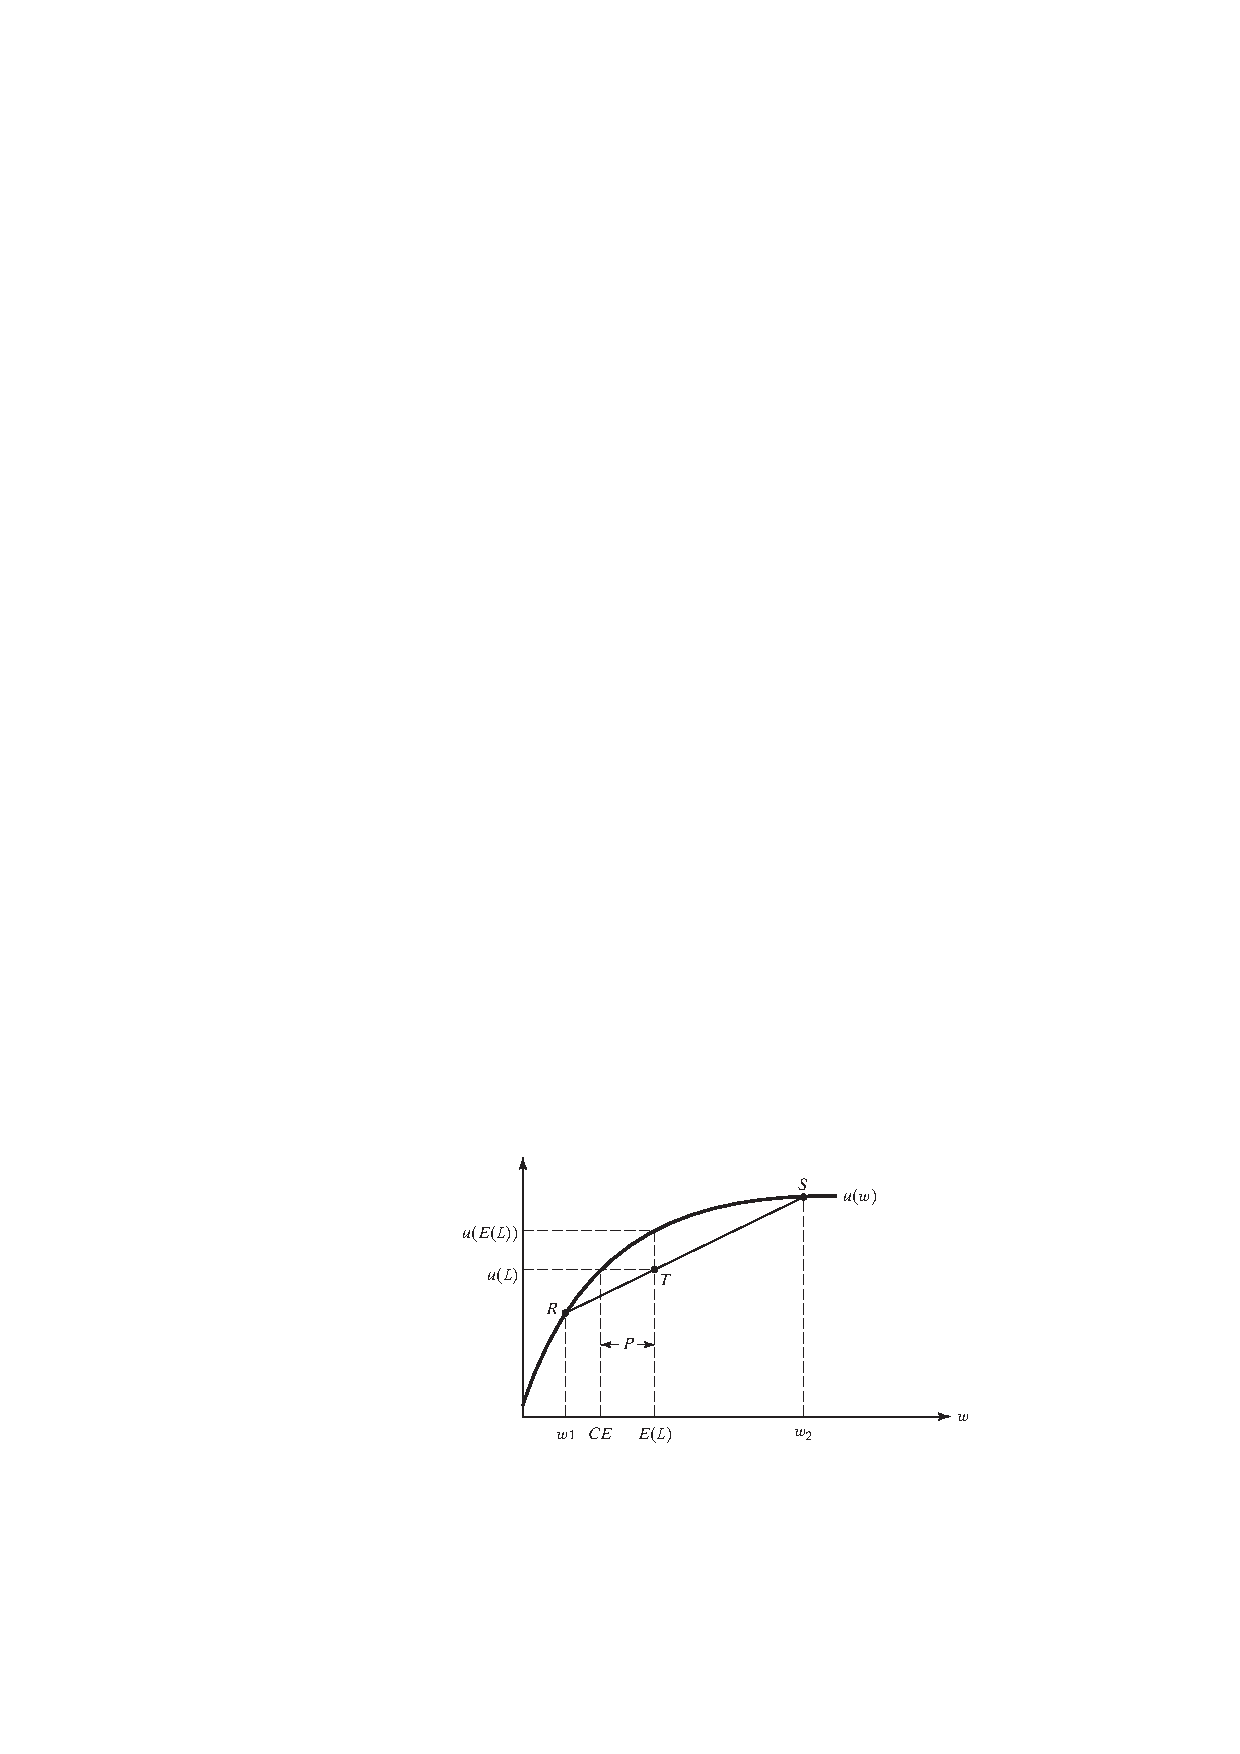
\includegraphics[width=10cm]{fig2-5.pdf}
  \caption{风险厌恶及严格凹的vNM效用函数.}\label{fig2.5}
\end{figure}

\begin{definition}[确定性等价与风险溢价]
任何定义在财富水平上的简单彩票的确定性等价是确定性地提供财富CE, 使得$u(L)=u(\text{CE})$. 风险溢价是一定量的财富水平$P$, 使得$u(L)=u(E(L)-P)$. 显然, $P=E(L)-\text{CE}$.
\end{definition}

\begin{example}
假设$u(w)=\ln w$, 由于这个函数是严格凹的, 因此消费者风险厌恶. 假设消费者的初始财富为$w_0$, 彩票$L=(0.5\circ (w_0+h), 0.5\circ (w_0-h))$, 那么$E(L)=w_0$, $L$的确定性等价必定满足
$$\ln \text{CE}=0.5\ln (w_0+h)+0.5\ln (w_0-h)=0.5\ln (w_0^2-h^2)$$
因此$\text{CE}=\sqrt{w_0^2-h^2}<E(L)$, 并且$P=w_0-\sqrt{w_0^2-h^2}>0$.
\end{example}

很多时候, 我们不仅向知道某个人是否厌恶风险, 而且想知道他厌恶风险的程度, 下面给出它的数学刻画. 假设消费者的初始财富为$w$, 彩票$L=(p\circ (w+h), (1-p)\circ (w-h))$, 于是vNM效用函数
\begin{equation}\label{eq2.33}
  u(w)=pu(w+h)+(1-p)u(w-h)
\end{equation}
将$u(w+h)$和$u(w-h)$分别在$w$处二阶Taylor展开得到
\begin{align*}
u(w+h)&=u(w)+hu'(w)+\frac{h^2}{2}u''(w)+o(h^2) \\
u(w-h)&=u(w)-hu'(w)+\frac{h^2}{2}u''(w)+o(h^2)
\end{align*}
忽略高阶余项后将其代入到式(\ref{eq2.33})有
$$u(w)=p\left[u(w)+hu'(w)+\frac{h^2}{2}u''(w)\right]+(1-p)\left[u(w)-hu'(w)+\frac{h^2}{2}u''(w)\right]$$
从中可以解出
$$p=\frac{1}{2}+\frac{h}{4}\left[-\frac{u''(w)}{u'(w)}\right]$$
这里的$p$就可以视为对决策者风险厌恶的度量, 越大的$p$值可以吸引越多的决策者购买彩票.
\begin{definition}[Arrow-Pratt风险测度]
设效用函数$u:\R_+\to \R$二阶可微, 则Arrow-Pratt风险测度为
$$R_a(w)=-\frac{u''(w)}{u'(w)}$$
又称为绝对风险厌恶系数 (coefficient of absolute risk aversion).
\end{definition}
可以证明, 当消费者厌恶风险、风险中性或喜爱风险时, $R_a(w)$的符号分别为正、零或负, 而且效用函数的任何正仿射变换都不会改变这个测度.

除了绝对量的彩票损益外, 我们还考虑彩票带来的损益与决策者的初始财富$w$成正比的情形, 也即彩票为$L=(p\circ (w+\theta w),(1-p)\circ (w-\theta w))$, 于是
$$u(w)=pu(w+\theta w)+(1-p)u(w-\theta w)$$
运用Taylor展开的技术可得
$$p=\frac{1}{2}+\frac{\theta}{4}\left[-\frac{wu''(w)}{u'(w)}\right]$$
我们称
$$R_R(w)=-\frac{wu''(w)}{u'(w)}$$
为\textbf{相对风险厌恶系数} (coefficient of relative risk aversion).

\begin{example}
假设某车主厌恶风险, 她的初始财富为$w_0$, vNM效用函数为$u$且二阶可微, 现在她需要决定是否购买车险. 假设她遭遇车祸的概率为$\alpha\in(0,1)$, 车祸损失为$l$, 则在公平的保险价格下, 她应该购买保险金额为多少的保险?

设$\rho$表示为1元保险金额的保险费, 也即花费$\rho$元购买保险, 风险发生时保险公司赔付1元钱, 于是保险公司的期望利润为$\alpha(\rho-1)+(1-\alpha)\rho$, 公平的保险价格要求保险公司利润为0, 解得$\rho=\alpha$, 也即每1元钱保险金额的保险费为$\alpha$.

设她购买的保险金额为$x$, 由于车主追求利润最大化, 因此期望效用
$$\alpha u(w_0-\alpha x-l+x)+(1-\alpha)u(w_0-\alpha x)$$
应该最大, 将上式关于$x$微分, 并令微分为0可得
$$(1-\alpha)\alpha u'(w_0-\alpha x-l+x)-\alpha(1-\alpha)u'(w_0-\alpha x)=0$$
也即
$$u'(w_0-\alpha x-l+x)=u'(w_0-\alpha x)$$
由于该车主是风险厌恶的, 因此$u''(w)<0$, 从而$u'(w)$单调递减, 因此
$$w_0-\alpha x-l+x=w_0-\alpha x$$
最终得到$x=l$, 也即在保险价格为精算公平价格下, 厌恶风险的个人将购买刚好覆盖全部损失的足额保险.
\end{example}

\begin{example}
假设某位投资者的初始资产为$w$, 风险资产的回报率为$r_i$ (可正可负), 每种回报结果发生的概率为$p_i>0$并且$\sum_{i=1}^{n}p_i=1$. 假设该投资者花了$\beta$购买风险资产, 则他在结果$i$下的财富变为
$$(w-\beta)+(1+r_i)\beta=w+\beta r_i$$
投资者的问题是选择合适的$\beta$, 使得财富带来的期望效用最大化, 也即
\begin{equation}\label{eq2.34}
  \max_\beta \sum_{i=1}^{n}p_iu(w+\beta r_i)\quad \text{s.t.}\quad 0\leq \beta\leq w
\end{equation}
其中$u$为二阶可微的vNM效用函数.

首先明确投资者何时不投资任何风险资产, 此时$\beta^\ast=0$, 将式(\ref{eq2.34})的期望效用对$\beta$微分, 然后求微分在$\beta^\ast=0$的值可得
$$\sum_{i=1}^{n}p_ir_iu'(w+\beta^\ast r_i)=u'(w)\sum_{i=1}^{n}p_ir_i\leq 0$$
由于$u'(w)$严格为正, 因此当且仅当风险资产的期望回报非正时, 风险厌恶的投资者不会购买风险资产.

现在假设风险资产的期望回报为正, 这意味着$\beta^\ast\neq 0$, 假设$\beta^\ast<w$, 故而内部最优解的一阶条件和二阶条件为
\begin{equation}\label{eq2.35}
  \sum_{i=1}^{n}p_ir_iu'(w+\beta^\ast r_i)=0
\end{equation}
以及
\begin{equation}\label{eq2.36}
\sum_{i=1}^{n}p_ir_i^2u''(w+\beta^\ast r_i)<0
\end{equation}
其中二阶条件用到了$u$关于$\beta$是凹函数的这一事实.

当投资者的财富水平增加时, 他用于购买风险资产的财富量将会发生什么样的变化? 可以证明, 随着财富水平的增加, 投资者将增加购买风险资产的绝对财富量, 也即风险资产是正常品而非劣等品.

将$\beta^\ast$视作$w$的函数, 在式(\ref{eq2.35})两端求$\beta^\ast$关于$w$的微分得到
\begin{equation}\label{eq2.37}
  \frac{\text{d}\beta^\ast}{\text{d}w}=-\frac{\sum_{i=1}^{n}p_ir_iu''(w+\beta^\ast r)}{\sum_{i=1}^{n}p_ir_i^2u''(w+\beta^\ast r)}
\end{equation}
风险厌恶保证了式(\ref{eq2.37})的分母为负, 因此当且仅当分子部分为正时, 风险资产是正常品, 这要求投资者是绝对风险厌恶递减的.

注意到恒等式
$$u''(w+\beta^\ast r_i)r_i=R_a(w+\beta^\ast r_i)u'(w+\beta^\ast r_i)r_i$$
在绝对风险厌恶递减下, 当$r_i>0$时有$R_a(w)>R_a(w+\beta^\ast r_i)$, 并且当$r_i<0$时有$R_a(w)<R_a(w+\beta^\ast r_i)$, 因此总有
\begin{equation}\label{eq2.38}
  R_a(w)r_i>R_a(w+\beta^\ast r_i)r_i
\end{equation}
由式(\ref{eq2.37})和(\ref{eq2.38})可得
$$u''(w+\beta^\ast r_i)r_i>-R_a(w)u'(w+\beta^\ast r_i)r_i$$
上式两端取期望得到
$$\sum_{i=1}^{n}p_ir_iu''(w+\beta^\ast r_i)>-R_a(w)\sum_{i=1}^{n}p_ir_iu'(w+\beta^\ast r_i)=0$$
这就完成了证明.

\end{example}
\subsection{随机占优}
期望效用理论给了我们判断随机回报在投资者眼中孰优孰劣的依据, 但期望效用依赖于投资者的偏好, 我们在这里想问的问题是, 有没有一种不依赖于投资者的偏好而比较两个随机回报的方法?

更具体地, 有没有办法说一个随机回报比另一个回报更好, 从而使得所有投资者 (即使是风险厌恶者)都偏好于前者? 有没有办法说一个随机回报比另一个回报风险更低, 从而使得所有风险厌恶的投资者都偏好于前者? 本节介绍的\textbf{随机占优 }(stochastic dominance)理论就可以回答这些问题.

我们知道财富$w$的累积分布函数$F(w)$可以用来描述彩票, 例如彩票
$$L=(0.25\circ 1, 0.5\circ 4, 0.25\circ 6)$$
可用
$$F(w)=\begin{cases}
         0, & w\in (-\infty,1) \\
         0.25, & w\in [1,4) \\
         0.75, & w\in [4,6) \\
         1, & w\in[6,\infty)
       \end{cases}$$
进行表示, 其中$U(w)$是非负财富水平的效用函数 (称为Bernoulli效用函数), 并且它是递增且连续的, 称为Bernoulli效用函数. 对于财富水平$w$, $F(w)$是获取小于等于财富水平$w$的概率.

\begin{definition}[一阶随机占优]
对于两个随机分布$F$和$G$, 如果对于任意非减函数$u:\R\to\R$都有
$$\int U(w)\,\text{d}F(w)\geq \int U(w)\,\text{d}G(w)$$
那么$F$对$G$是一阶随机占优的 (First Stochastic Dominance, FSD).
\end{definition}
FSD表明随机分布$F$产生的报酬明确地比分布$G$的报酬更高, 也即对于每个财富水平$w$, 在$F$下得到财富$w$的概率大于等于在$G$下得到的概率.

\begin{theorem}
  累计分布$F$一阶随机占优于$G$, 当且仅当对于每个$w$都有$F(w)\leq G(w)$.
\end{theorem}
\begin{proof}
  给定$F$和$G$, 再令$H(w)=F(w)-G(w)$. 假设对于某个$\overbar{w}$有$H(\overbar{w})>0$, 那么可以定义非减函数
  $$U(w)=\begin{cases}
           1, & w>\overbar{w} \\
           0, & w\leq\overbar{w}
         \end{cases}$$
  于是
  $$\int U(w)\,\text{d}H(w)=-H(\overbar{w})<0$$
  这就证明了必要性部分.

  现在来看充分性的部分, 首先不加证明地指出只要我们能够证明相应等价关系对于可微效用函数$u(w)$成立就足够了. 根据分部积分法可得
  $$\int U(w)\,\text{d}H(w)=\left.U(w)H(w)\right|_0^\infty-\int U'(w)H(w)\,\text{d}w$$
  由于$\displaystyle \lim_{w\to\infty}H(w)=0$且$H(0)=0$, 故而上式第一项为0. 另一方面, 假设$H(w)\leq0$且$U(w)$是递增的, 故而$\int U'(w)H(w)\,\text{d}w\leq0$, 由此可得上式第二项大于等于0, 因此
  $$\int U(w)\,\text{d}H(w)\ge0$$
  这就完成了证明.
\end{proof}
以上定理表明, 对于所有人, 不管他是风险厌恶还是风险喜爱, 都会对一阶随机占优的分布有更高的期望效用水平. 换言之, 在两个随机收益之间如果存在一阶随机占优的关系, 所有人都会选择一阶随机占优的那个随机收益.
\begin{example}
对于彩票$L_1=(0.4\circ 1, 0.3\circ 2, 0.3\circ 3)$和$L_2=(0.4\circ 1, 0.5\circ2, 0.1\circ 3)$, $L_1$和$L_2$的期望收入分别为190和170, 但彩票$L_1$的收益方差大于$L_2$的, 因此无法在均值方差框架下对$L_1$和$L_2$排序. 然而, 这两个彩票的累积分布函数为
$$F(w)=\begin{cases}
         0, & w\in (-\infty,1) \\
         0.4, & w\in [1,2) \\
         0.7, & w\in [2,3) \\
         1, & w\in[3,\infty)
       \end{cases},\quad G(w)=\begin{cases}
         0, & w\in (-\infty,1) \\
         0.4, & w\in [1,2) \\
         0.9, & w\in [2,3) \\
         1, & w\in[3,\infty)
       \end{cases}$$
因此$F$关于$G$是一阶随机占优的.
\end{example}

FSD涉及的思想是“较高/较好”对“较低/较差”, 下面我们试图引入另外一种比较方法, 这种方法建立在相对风险或者相对分散度上, 称为二阶随机占优.

\begin{definition}[二阶随机占优]
给定两个分布$F$和$G$, 它们的均值相同, 如果对于每个非减的凹函数$U:\R_+\to\R$都有
$$\int U(w)\,\text{d}F(w)\geq\int U(w)\,\text{d}G(w)$$
那么$F$对$G$是二阶随机占优的 (Second Stochastic Dominance, SSD), 或者说$F$的风险小于$G$.
\end{definition}

根据随机占优的定义, FSD意味着SSD, 但是反过来SSD并不一定意味着FSD. 例如对于随机变量$X_i\in \mathcal{N}(0,\sigma_i^2)$, $i=1,2$, $\sigma_1^2<\sigma_2^2$, 可以证明$F_{X_1}$二阶随机占优于$F_{X_2}$, 但$F_{X_1}$并不一阶随机占优于$F_{X_2}$.

\begin{definition}[保均展形]
随机变量$w$是随机变量$x$的保均展形 (mean-preserving spread), 当且仅当存在随机变量$z$使得$w=x+z$, 且对$x$的任意实现值$\tilde{x}$都有$E(z|\tilde{x})=0$.
\end{definition}

\begin{example}
考虑随机变量
$$x=\begin{cases}
      4, & p=0.5 \\
      1, & p=0.5
    \end{cases},\quad z=\begin{cases}
                          1, & p=0.5 \\
                          -1, & p=0.5
                        \end{cases}$$
从而随机变量
$$w=x+z=\begin{cases}
          5, & p=0.25 \\
          3, & p=0.25 \\
          2, & p=0.25 \\
          0, & p=0.25
        \end{cases}$$
尽管$E(x)=E(w)=2.5$, 但是$w$的风险看起来更大一些.
\end{example}

\begin{theorem}
  对于累计分布$F$和$G$, 如果它们的均值相等, 那么$F$二阶随机占优于$G$, 当且仅当$G$是$F$的保均展形.
\end{theorem}
这里不加证明地给出此定理, 表明如果两个随机收益之间存在二阶随机占优的关系, 那么所有风险厌恶者都会选择二阶随机占优的那个随机收益, 可见二阶随机占优是比一阶随机占优更弱的比较关系.

\chapter{厂商理论}
\section{生产}
厂商是将生产要素转变为产品的过程. 厂商在生产过程中必须面对的基本现实是技术可行性, 技术状况决定和限制了如何联合要素生产产品.

一般地, 厂商有一个\textbf{生产可能集} (production possibility set), 记作$Y\subset\R^m$, 并且$Y$中的每个向量$\mathbold{y}=(y_1,\cdots,y_m)'$称为一个\textbf{生产计划} (production plan), 每一个分量表示生产过程中的投入品或产出品, 我们用正数表示产出, 负数表示投入, 零表示该元素在生产过程中没有被用到. 尽管目前描述厂商技术的最一般方法是生产可能集, 我们通常考虑的是企业使用多种投入生产一种产品的情形, 此时使用\textbf{生产函数} (production function)描述企业的技术更为方便.

当使用多种生产要素来生产一种商品时, 可以用$y$表示产量, $x_i$表示生产要素$i$的投入量, $\x=(x_1,\cdots,x_n)$表示整个生产要素投入向量. 通常, 我们假设投入向量和产量必须非负, 也即要求$\x\ge \mathbf{0}$和$y\ge0$. 当我们写下$y=f(\x)$时, 我们的意思是说使用投入向量$\x$最多可以生产$y$单位产品. 此外, 我们还需要对生产函数施加一定限制.

\begin{definition}[生产函数]\label{def:def3.1}
生产函数$f:\R_n^+\to\R$在$\R_n^+$上是连续、严格递增和严格拟凹的, 并且$f(\mathbf{0})=0$.
\end{definition}

$f$的连续性是说投入向量的微小变化导致的产量变化也是微小的, 我们要求$f$为严格递增的, 目的是保证如果每种要素的投入量都严格增加, 则产量也严格增加. $f$为严格拟凹的, 则主要出于简化分析的需要. 与消费者的偏好为严格凸的假设类似. 当然, 如果不使用这条假设也可以, 它对我们的结论没有多大的影响. 最后, $f(\mathbf{0})=0$表明正的产量要求某些要素的投入量是正的.

如果还假设生产函数是可微的, 则它的偏导数$\partial f(\x)/\partial x_i$称为要素$i$的\textbf{边际产量} (marginal production), 它表示其它要素投入品不变时, 额外多使用一单位要素$i$所增加的产量. 由于生产函数$f$总是严格递增的, 因此$\partial f(\x)/\partial x_i>0$对几乎所有投入向量都成立, 表明投入品越多, 产量越高.

对于任何固定不变的产量水平$y$, 生产$y$单位产品的投入向量集称为$y$水平的\textbf{等产量线} (isoquant). 由此可见, 一条等产量线是$f$的一个水平集, 将其记为
$$Q(y)=\{\x\ge\mathbf{0}:f(\x)=y\}$$
对于一个投入向量$\x$, 通过$\x$的等产量线是由与向量$\x$生产相同产量$f(\x)$的所有投入向量组成的集合.

厂商理论中的\textbf{边际技术替代率} (Marginal Rate of Technology Substitution, MRTS)的概念类似于消费者理论中的边际替代率. MRTS衡量的是在产量不变的情形下要素$i$替代要素$j$的比率, 也即当投入要素为$\x$时, 要素$i$与要素$j$之间的边际技术替代率为
$$\text{MRTS}_{i,j}=\frac{\partial f(\x)/\partial x_i}{\partial f(\x)/\partial x_j}$$
如图\ref{fig3.1}所示, $\text{MRTS}_{12}(\x^1)$为通过$\x^1$的无差异曲线在点$\x^1$处斜率的绝对值.

\begin{figure}[htbp!]
  \centering
  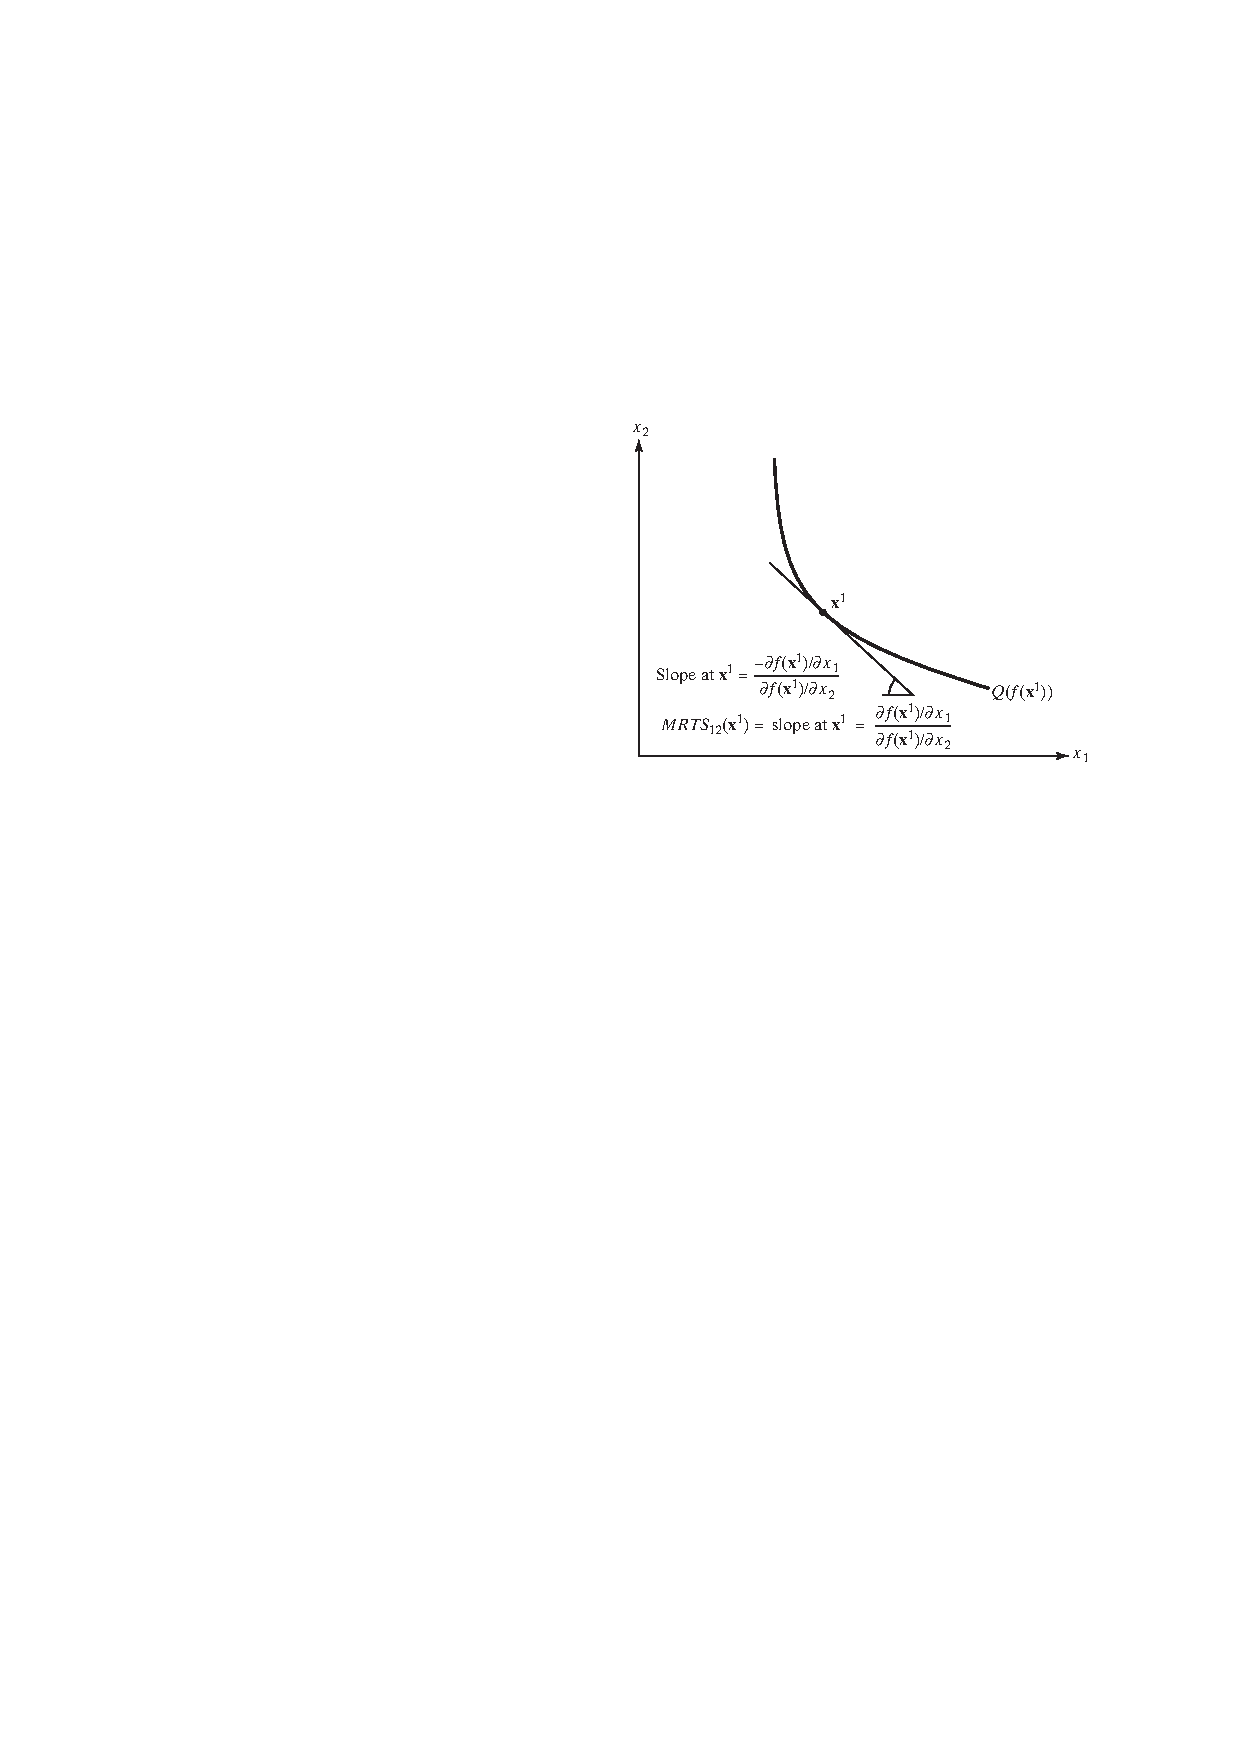
\includegraphics[width=9cm]{fig3-1.pdf}
  \caption{边际技术替代率.}\label{fig3.1}
\end{figure}

一般来说, 任何两种生产要素之间的$\text{MRTS}$取决于使用的所有生产要素. 然而, 最常见的做法是假设投入可以分为少数几种类型, 在某种给定类型的内部投入之间的替代程度, 和投入类型之间的替代程度是不同的, 称这样的生产函数是\textbf{可分的} (separable). 在下面的定义中, 我们将要素$i$的边际产量$\partial f(\x)/\partial x_i$简记为$f_i(\x)$.

\begin{definition}[可分性]
设$N=\{1,\cdots,n\}$是所有生产要素构成的集合, 这些要素可以分割为$S>1$个互不相交且将$N$穷尽的子集$N_1,\cdots,N_S$.
\begin{enumerate}[label=\arabic*.]
\item 如果同一子集中的任何两种要素的$\text{MRTS}$独立于其他组的要素, 也即
$$\frac{\partial [f_i(\x)/f_j(\x)]}{\partial x_k}=0,\quad \forall i,j\in N_s, k\notin N_s$$
那么称生产函数是弱可分的 (weakly separable).
\item 当$S>2$时, 如果两个不同子集中的任意两种要素的$\text{MRTS}$独立于这两个子集之外的其它要素, 也即
$$\frac{\partial [f_i(\x)/f_j(\x)]}{\partial x_k}=0,\quad \forall i\in N_s, j\in N_t, k\notin N_s\cup N_t$$
那么称生产函数是强可分的 (strongly separable).
\end{enumerate}
\end{definition}
MRTS只是在产量既定时生产要素之间替代性的一种局部衡量, 而经济学家特别喜欢用无单位的弹性衡量这样的事情, 尽管衡量方法有好几种, 目前最常见的方法是使用\textbf{替代弹性} (elasticity of substitution).

\begin{definition}[替代弹性]
 对于某个生产函数$f(\x)$, 要素$i$和$j$在点$\x^0\in\R_{++}^n$上的替代弹性为
 $$\sigma_{ij}(\x^0)=\left[\left.\frac{\text{d}\ln\text{MRTS}_{ij}(\x(r))}{\text{d}\ln r}\right|_{r=x_j^0/x_i^0}\right]^{-1}$$
 其中$\x(r)$是满足下列条件的唯一要素向量$\x=(x_1,\cdots,x_n)'$: i. $x_i/x_i=r$; ii. $x_k=x_k^0$, $k\neq i,j$; iii. $f(\x)=f(\x^0)$.
\end{definition}
替代弹性$\sigma_{ij}(\x^0)$衡量的是通过点$\x^0$的$i-j$无差异曲线在点$\x^0$处的曲率. 当生产函数为拟凹时, 替代弹性绝不会为负, 也即$\sigma_{ij}\ge0$. 一般地, 替代弹性越接近于0, 要素之间的替代越困难; 替代弹性越大, 要素之间的替代越容易.

在要素只有两种的情形下, 我们通常将替代弹性写成$\sigma$而不是$\sigma_{12}$. 在图\ref{fig3.2}(a)中, 等产量线是线性的, 要素之间完全可替代, 此时替代弹性$\sigma\to\infty$; 在(c)中, 两种要素只有以固定比例搭配才具有生产力, 它们之间不可能互相替代, 此时替代弹性$\sigma=0$; 在(b)中, 等产量线既非直线也非直角形状, 替代弹性$0<\sigma<\infty$.

一般地, $\sigma$越趋近于0, 无差异曲线越呈现L形, 要素之间越难相互替代; 反之, 如果$\sigma$越大, 无差异曲线越平坦, 要素之间越容易相互替代.

\begin{figure}[htbp!]
  \centering
  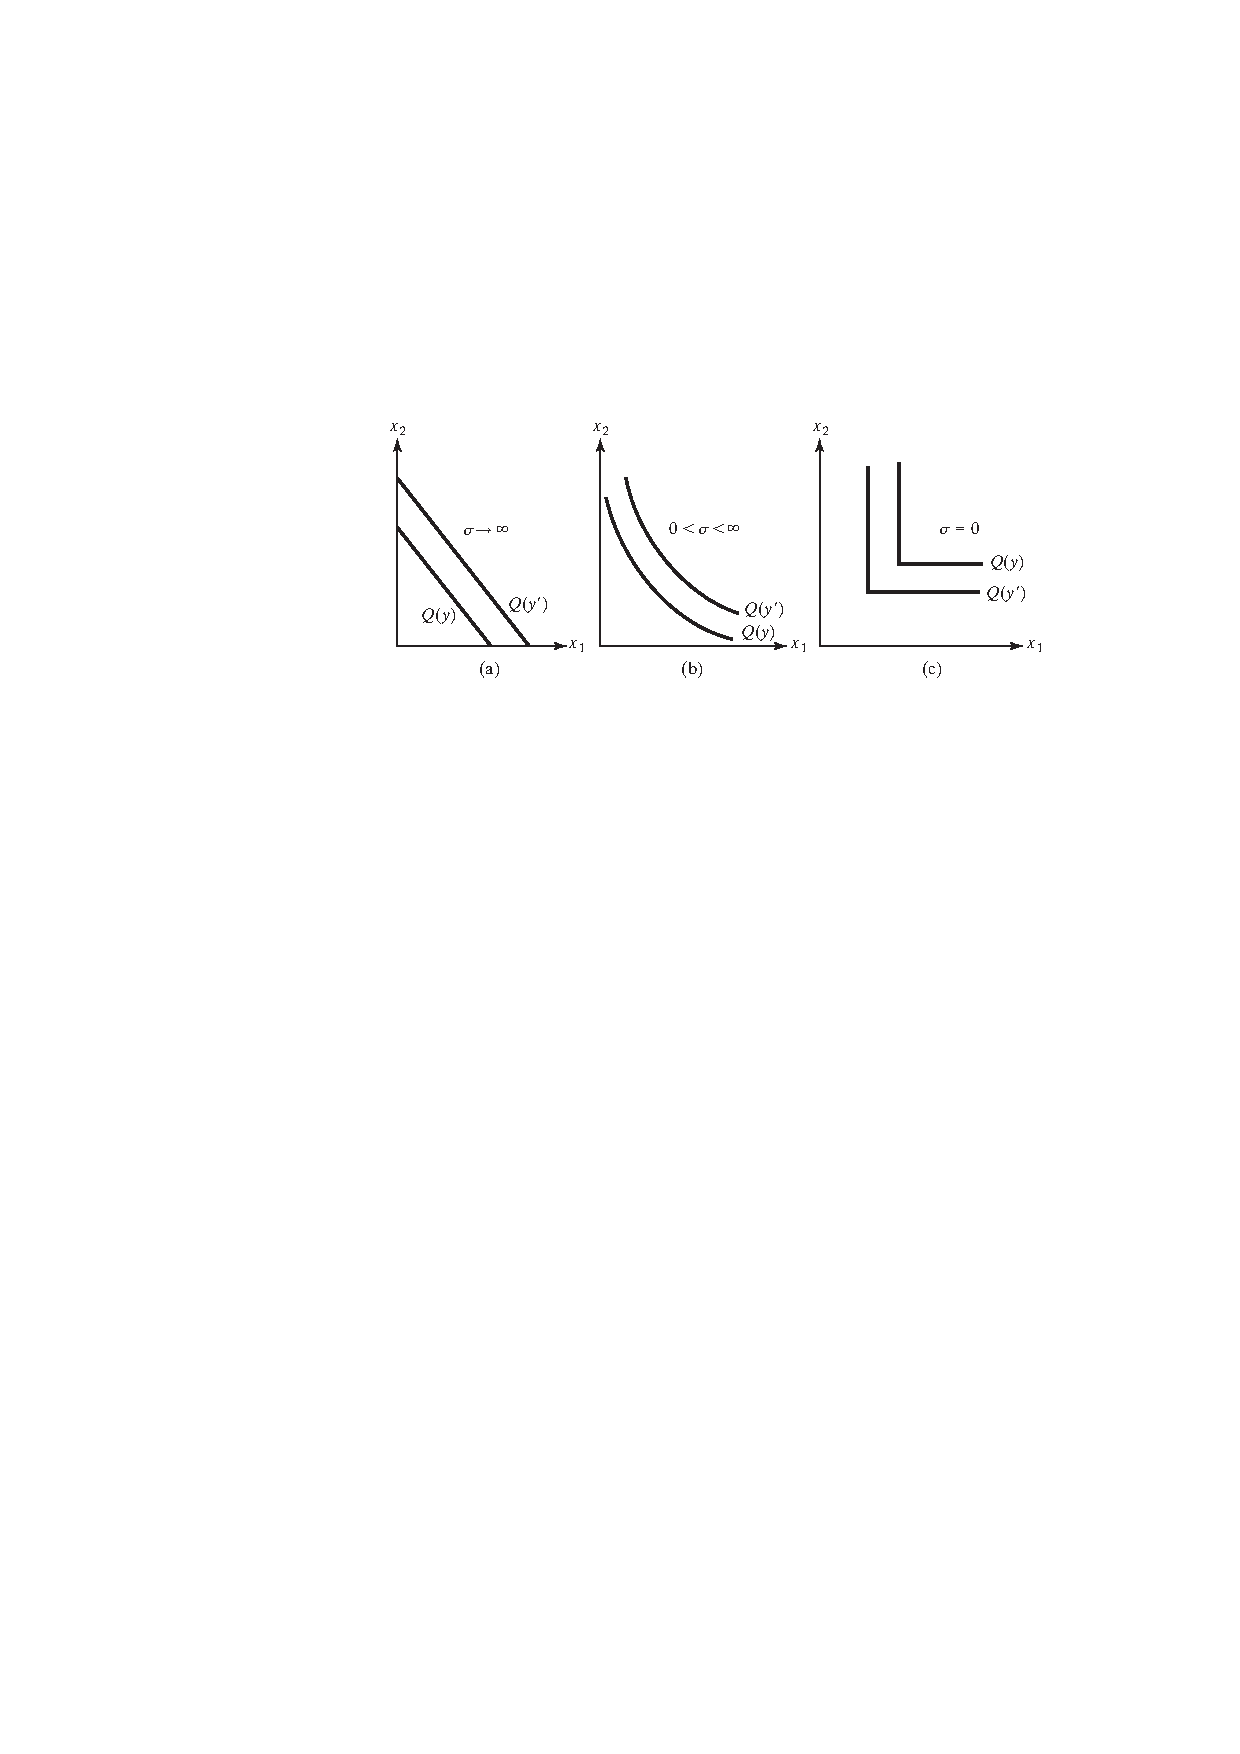
\includegraphics[width=12cm]{fig3-2.pdf}
  \caption{等产量线与替代弹性.}\label{fig3.2}
\end{figure}

\begin{example}[$\,$CES生产函数]
之前在消费者理论中已经讨论了CES效用函数, 这里将表明CES的含义是常替代弹性 (Constant Elasticity of Substitution, CES).

对于CES生产函数
$$y=(x_1^\rho+x_2^\rho)^{1/\rho},\quad 0\neq \rho<1$$
为了计算替代弹性$\sigma$, 首先注意到在任意点$(x_1,x_2)$上, 要素1和要素2之间的边际技术替代率为
$$\text{MRTS}_{12}(x_1,x_2)=\left(\frac{x_2}{x_1}\right)^{1-\rho}$$
这里两种要素的比值本身就决定了MRTS, 无论产量有多大. 因此, 我们令$r=x_2/x_1$, 于是
$$\frac{\text{d}\ln\text{MRTS}_{12}(\x(r))}{\text{d}\ln r}=\frac{\text{d}\ln r^{1-\rho}}{\text{d}\ln r}=1-\rho$$
因此
$$\sigma=\frac{1}{1-\rho}$$
可见在CES生产函数的情形下, 不论产量水平如何, 也不论要素投入之间的比例为多大,要素之间的替代程度总是一样的.
\end{example}

借助于上面的例子, 可以验证如果$\sum_{i=1}^{n}\alpha_i=1$, 那么
\begin{equation}\label{eq3.1}
  y=\left(\sum_{i=1}^{n}\alpha_ix_i^\rho\right)^{1/\rho}
\end{equation}
也是一个CES类型的生产函数, 并且替代弹性为$\sigma_{ij}=1/(1-\rho)$. 在式(\ref{eq3.1})两端取自然对数, 借助于L'Hospital法则, 可以证明当$\rho\to0$时, 式(\ref{eq3.1})变为具有线性齐次的Cobb-Douglas生产函数
$$y=\prod_{i=1}^{n}x_i^{\alpha_i}$$
此时的替代弹性$\rho_{ij}=1$. 当$\rho\to-\infty$时, $\sigma_{ij}\to 0$, 正是Leontief生产函数
$$y=\min\{x_1,\cdots,x_n\}$$
也即图\ref{fig3.1}(c)中的那样.

所有 CES类型的生产函数 (包括有限情形的Cobb-Douglas和Leontief生产函数)都是线性齐次生产函数族的元素, 这样的函数在理论和应用中非常重要. 此外, 线性齐次性为生产函数施加了很多额外的结构, 例如线性齐次生产函数总是凹函数.

\begin{theorem}
  对于定义\ref{def:def3.1}中的生产函数$f(\x)$, 如果它是$\alpha\in (0,1]$次齐次的, 那么它关于$\x$是凹的.
\end{theorem}
\begin{proof}
  首先假设$\alpha=1$, 即$f$是一次齐次的. 任取$\x^1,\x^2\gg\mathbf{0}$, 令$y^1=f(\x^1)$, $y^2=f(\x^2)$, 由于$f(\mathbf{0})=0$且$f$是递增的, 因此$y^1,y^2>0$. 因为$f$是一次齐次的, 故而
  $$f\left(\frac{\x^1}{y^1}\right)=f\left(\frac{\x^2}{y^2}\right)=1$$
  又因为$f$是拟凹的, 于是对一切$t\in[0,1]$都有
  \begin{equation}\label{eq3.2}
    f\left(\frac{t\x^1}{y^1+y^2}+\frac{(1-t)\x^1}{y^1+y^2}\right)\geq1
  \end{equation}
  现在选取$t^\ast=y^1/(y^1+y^2)$以及$1-t^\ast=y^2/(y^1+y^2)$, 根据式(\ref{eq3.2})可知
  \begin{equation}\label{eq3.3}
    f\left(\frac{\x^1+\x^2}{y^1+y^2}\right)\ge1
  \end{equation}
  再次使用$f$是一次齐次的条件, 根据式(\ref{eq3.3})可知
  \begin{equation}\label{eq3.4}
    f(\x^1+\x^2)\geq y^1+y^2=f(\x^1)+f(\x^2)
  \end{equation}
  由于$f$的连续性, 式(\ref{eq3.4})不仅对一切$\x^1,\x^2\gg\mathbf{0}$成立, 还对所有$\x^1,\x^2\ge\mathbf{0}$成立.

  现在考虑任意要素向量$\x^1,\x^2\ge\mathbf{0}$以及实数$t\in[0,1]$, 由一次齐次可得
  \begin{align*}
  f(t\x^1)&=tf(\x^1) \\
  f((1-t)\x^2)&=(1-t)f(\x^2)
  \end{align*}
  再由式(\ref{eq3.4})可得
  $$f(t\x^1+(1-t)\x^2)\geq tf(\x^1)+(1-t)f(\x^2)$$
  这就证明了$\alpha=1$时的结论. 现在考虑$f$是$\alpha\in (0,1]$次齐次的, 那么$f^{\frac{1}{\alpha}}$是一次齐次的, 并且符合定义\ref{def:def3.1}对生产函数的要求, 根据前面的结论可知$f^{\frac{1}{\alpha}}$是凹的, 这样一来$f=(f^{\frac{1}{\alpha}})^\alpha$也是凹的, 因为$\alpha\leq1$.
\end{proof}

我们经常想知道产量如何随不同要素的数量的变动而变动. 在\textbf{短期} (short run), 至少有一种要素固定不变, 产量的变动只能通过改变某些要素的数量来完成, 因为另外一些要素数量固定不变, 无法调整. 当可变要素的数量变动时, 固定要素和可变要素的比例也是变动的, 而\textbf{可变比例报酬} (return to variable proportions)可以描述产量如何随着这一比例的变动而变动. 在\textbf{长期} (long run), 厂商可以变动所有的要素, 此时描述产量如何作出反应的一种方法是将生产函数按照\textbf{规模报酬} (return to scale)进行分类, 它是指所有要素按相同比例变化时, 产量发生的变化.

如图\ref{fig3.3}所示, 可变比例报酬指的是沿着水平线$\overbar{x}_2$穿过等产量线族, 即保持$x_2$不变而只变动$x_1$的投入量时, 产量发生的变动. 规模报酬指的是沿着某条射线OA穿过等产量线族时, 即要素$x_1$, $x_2$同时发生变动但比例$x_2/x_1=\alpha$不变时, 产量发生的变动.

\begin{figure}[htbp!]
  \centering
  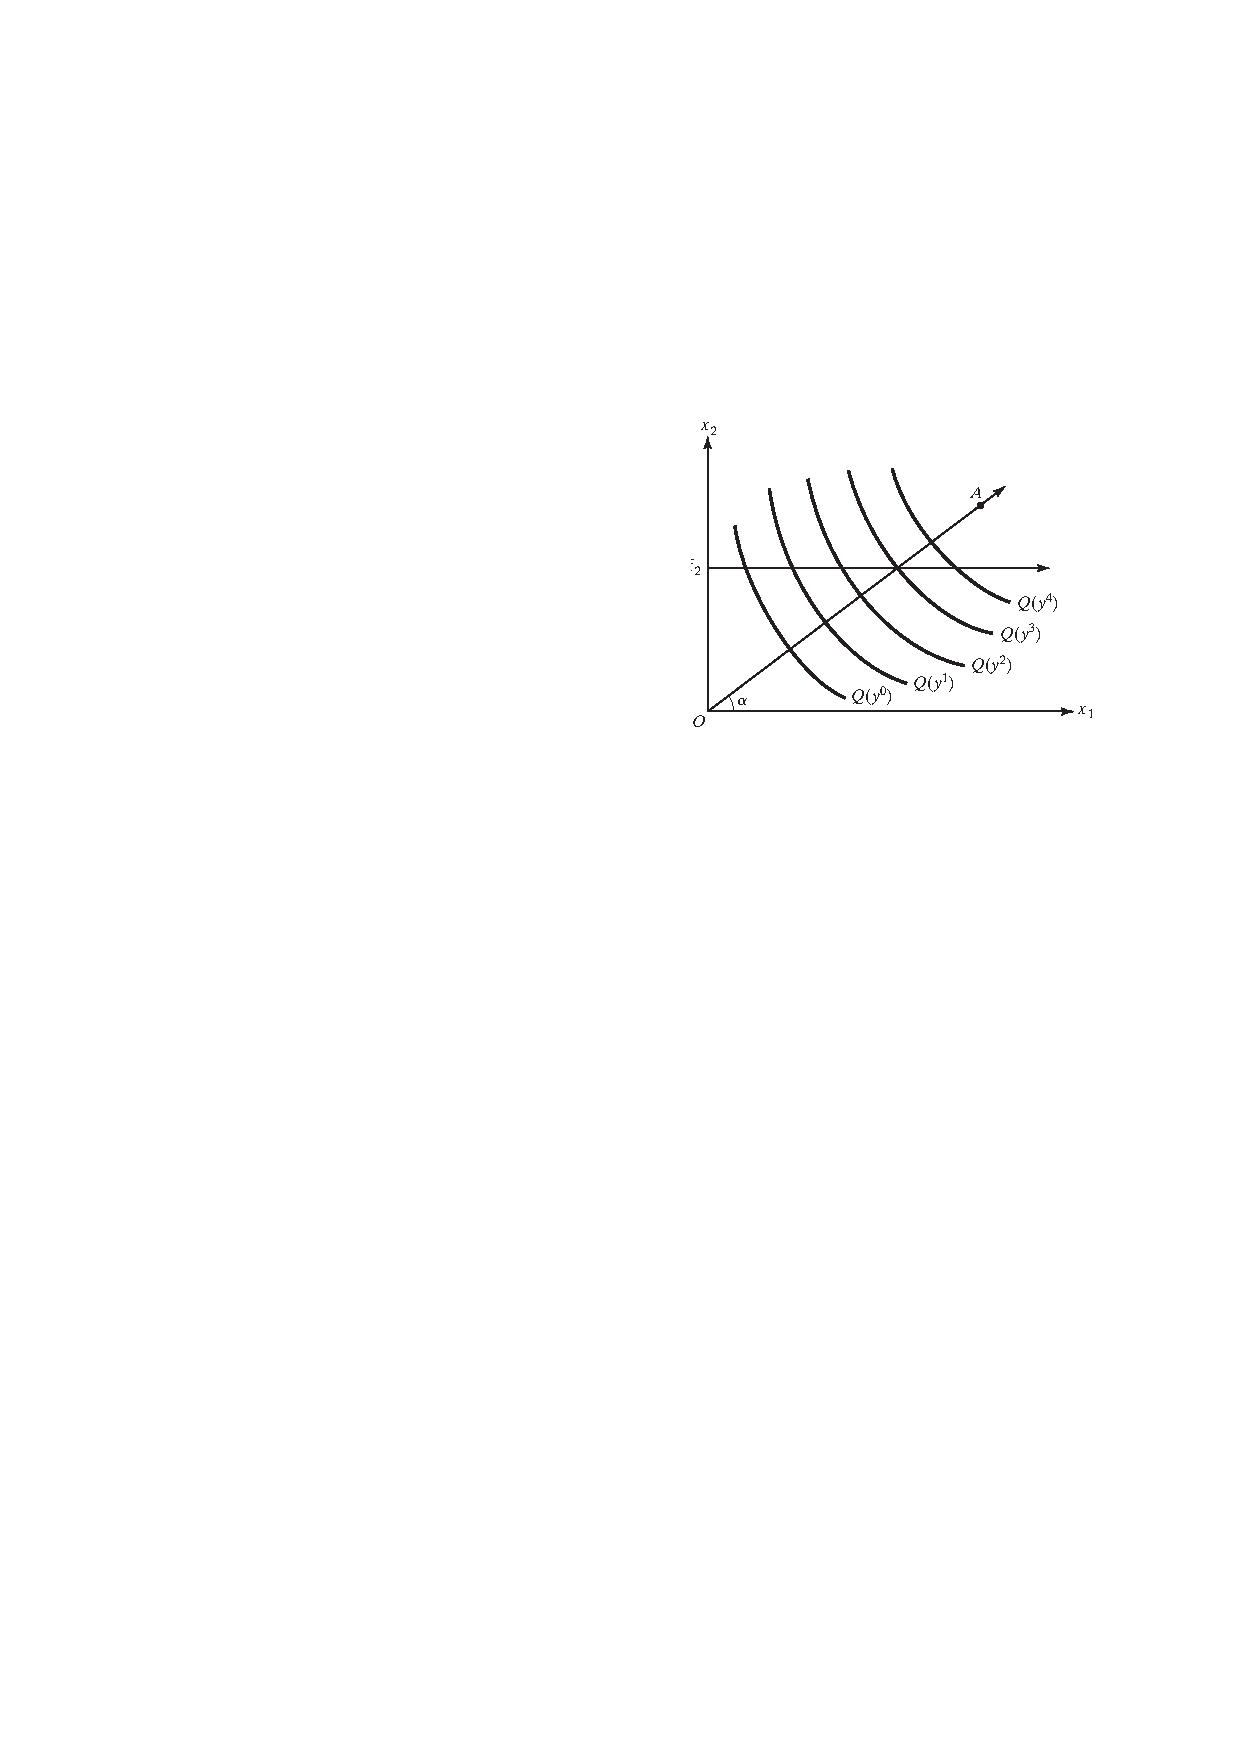
\includegraphics[width=9cm]{fig3-3.pdf}
  \caption{可变比例报酬与规模报酬.}\label{fig3.3}
\end{figure}

可变比例报酬的基本衡量指标包括每种生产要素的\textbf{边际产量}$\text{MP}_i(\x)=f_i(\x)$和\textbf{平均产量}$\text{AP}_i(\x)=f(\x)/x_i$. 此外, \textbf{要素产出弹性}$\mu_i(\x)=f_i(\x)/f(\x)=\text{MP}_i(\x)/\text{AP}_i(\x)$指的是它变化1\%时, 导致产量变动的百分数. 以上三种指标都是局部指标, 而生产技术的规模性质既可以是局部的, 也可以是全局的.

\begin{definition}[全局性的规模报酬]
生产函数$f(\x)$是全局性的
\begin{enumerate}[label=\arabic*.]
  \item 规模报酬不变, 如果对一切$t>0$和$\x$都有$f(t\x)=tf(\x)$;
  \item 规模报酬递增, 如果对一切$t>1$和$\x$都有$f(t\x)>tf(\x)$;
  \item 规模报酬递减, 如果对一切$t>1$和$\x$都有$f(t\x)<tf(\x)$.
\end{enumerate}
\end{definition}

可以看出, 如果某个生产函数是一次齐次的, 那么它具有规模报酬不变的特征. 而大于 (小于)一次的齐次生产函数必然是规模报酬递增 (递减的), 但是反过来不成立, 也就是说我们不能仅根据某个函数是规模报酬递增的就认为它是$>1$次的齐次生产函数.

另一方面, 定义\ref{def:def3.1}中的很多生产函数不属于上面任何一个情形. 很多生产技术只在某个产量区间呈现规模报酬递增、不变或递减, 因此还需要用到局部性的规模报酬概念, 其中一种衡量方式是\textbf{规模弹性} (elasticity of scale).

\begin{definition}[局部性的规模报酬]
在点$\x$处的规模弹性为
$$\mu(\x)=\lim_{t\to1}\frac{\text{d}\ln f(t\x)}{\text{d}\ln t}=\frac{\sum_{i=1}^{n}x_if_i(\x)}{f(\x)}$$
当$\mu(\x)$大于、等于或小于1时候, 分别称规模报酬是局部递增、局部不变或局部递减的. 可以看出, 要素产出弹性和规模弹性的关系为
$$\mu(\x)=\sum_{i=1}^{n}\mu_i(\x)$$
\end{definition}

\begin{example}
考虑生产函数
\begin{equation}\label{eq3.5}
  y=k(1+x_1^{-\alpha}x_2^{-\beta})^{-1}
\end{equation}
其中$\alpha,\beta>0$, $0\leq y\leq k$是产量的上界. 每种要素的产出弹性可得
\begin{align}
\begin{split}
\mu_1(\x)&=\alpha(1+x_1^{-\alpha}x_2^{-\beta})^{-1}x_1^{-\alpha}x_2^{-\beta} \\
\mu_2(\x)&=\beta(1+x_1^{-\alpha}x_2^{-\beta})^{-1}x_1^{-\alpha}x_2^{-\beta}
\end{split}
\label{eq3.6}
\end{align}
从上式可以看出, 要素产出弹性显然取决于规模和要素投入比例. 将上面的两个式子相加即可得到规模弹性
$$\mu(\x)=(\alpha+\beta)(1+x_1^{-\alpha}x_2^{-\beta})^{-1}x_1^{-\alpha}x_2^{-\beta}$$
显然, 规模弹性也取决于$\x$.

从另一个角度看, 可以将弹性看成是产量的函数, 此时可以由式(\ref{eq3.5})得到更简约的表达式
\begin{equation}\label{eq3.7}
  x_1^{-\alpha}x_2^{-\beta}=\frac{k}{y}-1
\end{equation}
将式(\ref{eq3.5})和(\ref{eq3.7})代入到(\ref{eq3.6})可得
\begin{align*}
\mu_1^\ast(y)&=\alpha\left(1-\frac{y}{k}\right) \\
\mu_2^\ast(y)&=\beta\left(1-\frac{y}{k}\right)
\end{align*}
相加可得规模弹性
$$\mu^\ast(y)=(\alpha+\beta)\left(1-\frac{y}{k}\right)$$
显然, 每种要素的报酬, 以及总规模报酬都是随着产量增加而单调递减的, 当$y=0$时有$\mu^\ast(y)=\alpha+\beta$, 而当$y\to k$时有$\mu(y)\to 0$.

进一步, 如果$\alpha+\beta>1$, 对于较低的产量水平$\displaystyle 0\leq y<k\left(1-\frac{1}{\alpha+\beta}\right)$, 该生产函数是规模报酬递增的, 在产量水平$\displaystyle y=k\left(1-\frac{1}{\alpha+\beta}\right)$上是规模报酬不变的, 而对于较低的产量水平$\displaystyle k\left(1-\frac{1}{\alpha+\beta}\right)<y<k$是规模报酬递减的.
\end{example}
\section{成本}
\chapter{局部均衡}

\chapter{一般均衡}

\chapter{社会选择与福利}

\chapter{博弈论}

\chapter{信息经济学}

\chapter{拍卖与机制设计}
\end{document} 